 % \iffalse
%%
%% This is the file `arlticle.cls',
%% composed by Steven B Segletes.
%%
%% Based on LaTeX's standard article.cls and an arltr class file obtained 
%% from Brian Krzewinski via Stephen Schraml...
%% this class file was modified quite a bit by Steven Segletes (March 2006).
%% It creates a LaTeX document class for the ARL-TR technical report series.
%% Documentation in the form of a dtx file was added April-May 2006.
%% Changes have been ongoing since its inception, at least through 
%% NOV 2016.
%%
%% Please treat this document as limited distribution.
%%
%% Steven may be reached at 278-6010 for questions comments and updates.
%%
%<*driver>
\ProvidesFile{arlticle.dtx}
%</driver>
%<class>\ProvidesClass{arlticle}
%(<*driver> | <*class>)
[2018/02/05 v2.43
       ARL Technical Report Document Class File]
\NeedsTeXFormat{LaTeX2e}
%(</driver> | </class>)
%<*driver>
% V1.23-Modified \sectionprelude to elevate \rule by 3mm
%      -Added ability to create one's own distribution list
%      -Modified initial length declarations to replace negative
%        \topmargin with zeroed \voffset, \headheight and \headsep.
%      -Declared twoside option, to achieve changed left/right page 
%        offset of 0.03in.
%      -Added ability to create one's own SF298
%      -Added the ability to create the ARL report cover(s), in
%        color, if desired
%      -Added standard journal title codes to ARL BibTeX style.
% V1.24-Automated Report Distribution Statements (\distcodes)
%      -spiffed up SF298 layout
% V1.25-fixed it so that \label calls in Appendix declarations produce
%        the appendix letter, when called via \ref.  Also fixed up 
%        subsection calls and figure/table/equation numbering 
%        within appendices.
% V1.26-Provided ability to provide top/bottom "page stamps" on each
%        page, which are to be used to indicate DRAFT or classification
%        marking
% V1.27-Fixed bug in \distcodes that caused extraneous chars to be printed.
%        Added fields 5a, 10, 11 to SFitems.
% V1.28-Modified code to allow for color to be added to PageStamp argument.
% V1.29-Modified code to provide 1.5ex intersentence spacing.
% V1.30-Made sure that inside front and back covers of classified
%        reports are labeled as UNCLASSIFIED.
%      -Added SFitemSIXTEENa, b, and c options.
%      -Changed size of pagestamp to \Large
%      -Added \downgrading command
%      -Added \UseClassMarkings command
% v1.31-Corrected margin sizes to account for v1.30 pagestamp size
% v1.32-Added support for full vs. abbreviated state-names in
%        \arlbibliography.
% v1.33-Corrected \@disclaimerpage so that any pagestamp *containing*
%       the words secret or confidential was marked UNCLASSIFIED for this
%       page only.  Previously required exact match to \thePageStamp.
%   (a)-Updated default Office Symbol to new nomenclature
%   (b)-added \widow & \orphan commands
% v1.34-Corrected SF298 defaults for items 16.
%      -Added \secref command, for section referencing without the
%       trailing period.
%      -Troubleshooting section added.
%      -Added \AddSpaceInCites command.
%   (a)-Changed \@pubdate default for the new decade
% v1.35-added \baresection command, like \section* + toc addition
% V1.36-corrected justification of export-control warning text, due to
%       missing '%' character
% V1.40-corrected \onehalfspace to \onehalfspacing to avoid dangling
%       open environment
%      -Added New Cover Logo to report
% V1.41-added color-logo covers with option {c} to \ARLcover
% V1.42-added \ARLaddress command, to allow specification of Adelphi
% V1.43-corrected logo-placement issue, which had resulted in improper
%       logo width on cover
% V1.44-added grayscale logo with option {g} to \ARLcover
% V1.45-fixed bug in ARLcover routine
% V1.46-defined default pubdate to real date, to prevent ARLcover from
%       choking
% V1.50-Revised/rewrote references environment for those not using
%       BibTeX
% V1.60-Reworked distribution list items to handle multiline entries
%       centering them.  Introduced \xdlitem, \pdlitem, \hdlitem, and
%       \ldlitem
% V1.61-Added \dlem for dist.list email names, and produced secondary
%       document to give distlist with email names included for TechPubs
% V1.62-Made \SFitemSEVENTEEN obsolete, instead setting value based on
%       specification of \distcodes.  Left placeholder for backward
%       compatibility.  Likewise for \SFitemFOUR, which now uses
%       \@arltitle and strips the linebreaks.
% V1.63-Avoided use of xpatch package, by explicitly patching definition
%       of \protected@write to make \protected@iwrite
% V1.64-Fixed use of \downgrading with new DL file feature
%      -Revised format of \downgrading
% V1.65-Added [p] option to \appendix and \appendix*
%      -Provided \freefootnote command
% V1.70-Changed references to "DoD" to "DOD".
%      -Used package [table]{xcolor} instead of {color}, to allow
%       colored table entries to be employed.
%      -Added \DLPageStamp for changing stamp (classification) of 
%       distribution list relative to prior page, since one cannot
%       effectively use \PageStamp between \distlistsetup
%       and \distlistcleanup.
%      -Adjusted \backcover so that inner back cover gets no page stamp.
% V1.71-Revised \distribution, to include "CLASSIFIED BY:" field
%      -Cleaned up \distcodes, also making it add C10 reason whenever
%       export control was invoked.
% V1.72-Provided \AddDistributionReason{} to augment reasons cited
%       in distribution list for limitation.
% V1.73-REVOKED auto-add of C10 reason to export-controlled docs,
%       based on pow-wow between ARL TechPubs and ARL Security.
% V1.74-Fixed bug in \distcodes introduced in V1.72, when using Dist A.
%      -Revised downgrading statement to remove underlining and bold
%       from text following colons.
% V1.75-Added hyphen to figure and table numbers in appendices
% V1.76-Added \FOIAexemptions{} macro.
%      -Make sure reverse page of ARL cover is not FOUO.
% V1.77 (incorporating V1.76x, V1.77x2 and V1.77x3)
%      -Introduced \citep citation macro, when citing material inside 
%       of parentheses; it will use [], not () (POC: Joel Stewart)
%      -Introduced \FOUOPageStamp[], defaulting to "FOR OFFICIAL USE ONLY"
%       at the page bottom only.  Other page-bottom markings may be
%       obtained through the use of the optional argument.
%      -Added vertical gap between FOIA exemption statement and export-
%       control warning text on cover and title page.
%      -Forced disclaimer page to show "UNCLASSIFIED" on an FOUO document.
%       (this seems wrong to me, so I left commented original code, if 
%       later this "style" is undone).
%      -Made List of Figures and List of Tables set their multi-line
%       captions in ragged right.
% V2.00 (Upgrade for Phase I of new ARL Report Style of 7/1/14)
%      -0.03" Binding margin removed.
%      -No more headers in distribution lists
%      -New mandatory distribution lists formulated, reflecting no page
%       break between mandatory and user distribution lists.
%      -Small alignment changes to SF-298 to conform to alignment guidelines
%      -Disclaimer page from \footnotesize to \small font size.
%      -French spacing used for single spacing after periods, colons.
%      -Citations superscripted (one of two acceptable ARL formats)
%      -Figure captions changed: "Fig. x This is the caption."
%      -Likewise for table captions.
%      -LOF and LOT revised to conform to new captioning label format.
%      -Helper routines (for removing dots) added for new bibliography style.
% V2.01-Removed period at the end of figure and table entries in lof and
%       lot.
%      -Removed period at the end of captions.
% V2.02-Made the [p] option of \appendix and \appendix* center the
%       appendix title horizontally on the page.
% V2.03-Use [nospace] option of cite package
% V2.04-Eliminated use of nonstandard "mycommands.tex"
% V2.05-Corrects spacing issues on title page with multi-line titles
%       and authors
%      -Adds possibility for four contributing organizations with
%       \authorsD and \organizationD
%      -Screens \freefootnote occurences in section titles from 
%       appearing in \tableofcontents
%      -Blank line is no longer required after section headings in
%       order to get proper line spacing
%      -Removes implicit dependency of \arltitlepage on calc package
%       (which is not otherwise specified in the class file)
% V2.10-(Update for Phase II of new ARL Report Style of 1/1/15)
%      -Uses OpenSans as the default sans serif font family
%      -New margin definitions throughout document
%      -Full justification of body text
%      -\setpreferredlineflush just passes through its argument, since
%       flushed text is the new standard
%      -\AddSpaceInCites is no longer active (since cites are superscripted)
%      -Section indent depth changed.
%      -Introduced \useOpenSans(default), \useLMss, \useCMss, \useCalibri
%      -Raggedright section, subsection headings
%      -Sans serif elements introduced: sectioning, contents, LOF, LOT,
%       cover, title page, SF298 header, page stamp, etc.
%      -New line structure (incl. color) in section, subsection headers
%      -Bold captions, no hanging indent.
%      -Introduced (optional with \sectspace) added  kern in section headings
%      -\spaceout{} macro for kerning out text provided
%      -Margin control now done exclusively with geometry package
%      -Introduced \def\PageStampColor{} as parameter
%      -FOIA exemption text revised
%      -Introduced conversion for \@pubdate into \@shortpubdate for report cover
%      -Now allow "X" as parameter for \AddDistributionReason
%      -Major revisions on Cover and Title Page.
%      -The macro \UnderContract{} provided to supply contract number
%      -Added macros for *ALL* SF-298 elements
%      -Replaced homegrown code for TOC, LOF, & LOT, with tocloft package
%       approach
%      -Made [p] option of \appendix the default: V- & H-centered appendix title
%      -Distribution list margins slightly revised
%      -Make 1.5 line spacing the class default, so not needed in user document.
%      -Removed \DLPageStamp logic (not needed).
%      -Removed alternate ways of making SF298
%      -Auto filled SF-298 blocks 5a and 6
% V2.11-Corrected flaw in \spaceout that changed global spacing with use of
%       optional argument
% V2.12-Corrected \pubdate to not throw an error with a blank argument
% V2.13-Made ReportColor and margins available, even when no Cover used
%       (e.g., in a test document)
% V2.14-Updated documentation to give up-to-date bibliography examples
%      -Made caption size \footnotesize, instead of \small
% V2.15-Updated cover design to reflect choice of smaller fonts
%      -When using \UnderContract, default Report No. set to ARL-CR-XXXX
%      -\NoBibDots revised to handle diacritics seamlessly (without \protect)
% V2.16-Detected issues with horizontal kern between sectioning numbers
%       and associated titles (it broke \secref).  After consulting
%       TechReports, LaTeX default of 1em sectioning gap was reinstated.
% V2.17-Eliminated the need for \secref by modifying \@seccntformat
% V2.18-Allowed for 5 organizations with \authorE, \organizationE
%      -Allowed for shrinkage of inter-author space.
% V2.19-Introduced \useSingleTable and \useSingleFigure to auto-revise caption, 
%       lof, and lot labels when only a single table or figure is employed.
%      -Introduced \FOUOunderset and its particular instance of 
%       \FOUOincludegraphics to place bold sffamily "FOUO" under an object
%       or a graphic, respectively.
%      -Revised \@disclaimerpage to make its page stamp empty on FOUO documents.
%      -Revised settings for obsolete "distlist" and "distlistend" page styles
%       to make them "plain", instead of "pagestamp".
%      -Changed occurences of "U.S." to "US".
%      -Fixed \baresection to call \addcontentsline outside of title.
% V2.20-Removed \NoBibDots logic after Matt Floros showed that the same 
%       function could be handled by ARL.bst with 
%       "{vv~}{ll}{~f}{~jj}" format.name$
% V2.21-Fixed placement of \SFitemSEVEN and \SFitemNINE to make for top
%       oriented placement (both now allow for 4 lines)
% V2.22-Added a low-ink-version of \ARLcover, using {0} as the argument.
% V2.23-Added \renewcommand\cftsecaftersnum{.} to add dot to toc sec. nos.
% V2.24-Added ARLtable and ARLfigure environments, which default to
%       \footnotesize and \centering.  Documented these additions.
% V2.25-Place abbreviated distribution statement at the bottom of each page, 
%       beginning with page iii.
% V2.26-Corrected bug with \spaceout code to allow trapping of \label and
%       \color properly.
% V2.27-Corrected bug in \@shortpubdate which did not detect/abbreviate the
%       month April to APR.
% V2.28-Made field 12 of SF298 ragged right
% V2.29-Provide for default abbreviated distribution statement used in footer
%       of pages from toc onward. The default is a call to used \distcodes.
%      -Fixed some redundant grammer in manual.
%      -Remind user in manual of workaround for cleveref conflicts with
%       \appendix and \appendix*.
% V2.30-Introduced \SFitemTWO{} for SF298 item 2, if needed.
%      -Auto detect \SFitemTWO (report type) by examining argument of \arlrptno, 
%       if possible.
% V2.31-Refined auto-detect of \SFitemTWO, to include more report types.
% V2.32-Stopped changing page stamp for Disclaimer Page.
%      -Added star variants for \listoftables and \listoffigures to suppress
%       leading \clearpage.
%      -Removed trailing \clearpage from \tableofcontents.
% V2.33-Added support for Level 4 sectioning (\paragraph) in the ARL style.
%      -Added support for (but left unactivated) level 4 tocdepth.
%      -Updated distribution reasons to reflect newest ARL Form 1 specification.
% V2.34-Removed the abbreviated distribution statement from the back cover
% V2.4 -Added MultipleSourcesMemo environment and \signMultipleSourcesMemo
%       macro.
%      -Made back cover uncolored.
% V2.41-Reworked vertical spacing of boilerplate text on cover and titlepage
% V2.42-Turned off abbreviated distribution when \downgrading is invoked.
%      -Adjusted MultipleSourcesMemo, to account for revised \downgrading
%       definition.
% V2.43-Made smaller the font size of Item 12 of the SF298, if it exceeds one line
% 
\documentclass{ltxdoc}
\usepackage{needspace,xcolor,verbatimbox}
\newcommand{\visavis}{\textit{vis-$\grave{a}$-vis}~}
\newcommand{\ie}{\textit{i.e.},~}
\newcommand{\etc}{\textit{etc.}}
\newcommand{\eg}{\textit{e.g.},~}
\newcommand\widow{\widowpenalty=10000\par\widowpenalty=150}
\DisableCrossrefs
\CodelineNumbered
\OnlyDescription
% DEFINE SOME COMMANDS THAT ARE EASIER HERE THAN IN DocInput ENVIRONMENT
\let\iq\itshape%     SHORTHAND FOR ITALIC  FONT
\let\uq\upshape%     SHORTHAND FOR UPSHAPE FONT
\newcommand\arlticle{\textsf{arlticle}~}
\newcommand\boxhandler{\textsf{boxhandler}~}
\newcommand\needspc{\textsf{needspace}~}
\begin{document}
   \DocInput{arlticle.dtx}
\end{document}
%</driver>
% \fi
% \GetFileInfo{arlticle.dtx} 
%    \title{
%           The \arlticle Document Class\\
%          \rule{0em}{0.7em}\small\fileinfo}
%    \author{Steven B. Segletes\\
%            steven@arl.army.mil}
%    \date{\filedate\\
%          \fileversion}
%    \maketitle
% \parskip 1ex
% \tableofcontents
% \begin{center} \rule{2in}{0.02in} \end{center}
% \section{Document-Class \textsf{arlticle}-Specific Commands}
% To begin, we will enumerate the 
% ARL Specific commands that can or must be included, as needed, in
% the .tex file that constitutes your ARL report.  These commands
% are new, in some cases, or reworked \visavis standard \LaTeX{} in
% other cases.
%
% \subsection{Front Matter}
% \subsubsection{Report Cover \& Title Page}
%|\arladdress{|\iq string\uq|}                |\\
%|\arlzipcode{|\iq string\uq|}                |\\
%|\arlrptno{|\iq string\uq|}                  |\\
%|\pubdate{|\iq string\uq|}                   |\\
%|\arltitle{|\iq string\uq|}                  |\\
%|\allauthors{|\iq string\uq|}                |\\
%|\authorsA{|\iq string\uq|}                  |\\
%|\organizationA{|\iq string\uq|}             |\\
%|\authorsB{|\iq string\uq|}                  |\\
%|\organizationB{|\iq string\uq|}             |\\
%|\authorsC{|\iq string\uq|}                  |\\
%|\organizationC{|\iq string\uq|}             |\\
%|\authorsD{|\iq string\uq|}                  |\\
%|\organizationD{|\iq string\uq|}             |\\
%|\authorsE{|\iq string\uq|}                  |\\
%|\organizationE{|\iq string\uq|}             |\\
%|\UnderContract{|\iq string\uq|}             |\\
%|\titlepagenote{|\iq string\uq|}             |\\
%|\distcodes[|\iq ofc.symbol\uq|]{|\iq dstr.letter\uq|}{|\iq dstr.number\uq
%                 |}{|\iq export.control\uq|} |\\
%|\AddDistributionReason{|\iq dstr.number\uq|}|\\
%|\distribution{|\iq string\uq|}              |\\
%|\PageStamp[|\iq string\uq|]                 |\\
%|\def\PageStampColor{|\iq color\uq|}         |\\
%|\StopPageStamp                              |\\
%|\FOUOPageStamp[|\iq string\uq|]             |\\
%|\FOIAexemptions{|\iq string\uq|}            |\\
%|\UseClassMarkings                           |\\
%|\downgrading{|\iq Classifying Individual\uq|}{|\iq Title\uq
%         |}{|\iq SCG\uq|}{|\iq Source date\uq|}{|\iq Declas. date\uq|}|\\
%|\useSingleFigure                            |\\
%|\useSingleTable                             |\\
%|\ARLcover[|\iq string\uq|]{|\iq code\uq|}   |\\
%|\arltitlepage                               |\\
%|\sectspace                                  |\\
%|\nosectspace                                |\\
%|\spaceout{|\iq string\uq|}                  |\\
%
% Note that as of \arlticle version 2.10, the proper sans serif font to
% be used in ARL \LaTeX{} reports is OpenSans, which the \arlticle 
% |\documentclass| will attempt to load.  If your \LaTeX{} installation
% cannot load this font, please contact Steven Segletes for further assistence.
%
% \DescribeMacro{\arladdress}
% Titlepage data.  Default Address is ``Aberdeen Proving Ground, MD
% 21005-5066.''  This will allow reset to other addresses, such as
% ``Adelphi, MD 20783-1197.''
%
% \DescribeMacro{\arlzipcode}
% Titlepage data.  Default Zipcode is 21005-5066.  Set the ZIPcode
% to that associated with your particular directorate/building (for APG
% use only).
%
% \DescribeMacro{\arlrptno}
% Cover and Titlepage Data.  You won't know your ARL report number until it
% is assigned,
% very close to publication.  At that point, enter data as the argument, 
% so that the report number page prints out correctly on the cover and
% title page.
%
% \DescribeMacro{\pubdate}
% Cover and Titlepage Data.  You won't know the official publication
% date of your
% report until it is assigned to you, close to publication.  At this
% point, enter the data as the argument, so that the cover and
% title page print out the publication date correctly.
%
% \DescribeMacro{\arltitle}
% Cover and Titlepage Data.  The argument is the title of your ARL report.
% Line breaks (|\\|) may be added to achieve proper appearance.
%
% \DescribeMacro{\allauthors}
% Cover Data. All authors of the report should be provided in the
% argument as a comma separated list of the form
% \{author1, author2, ..., and author-\textit{n}\}.  If needed, line
% breaks (|\\|) may be employed to separate the list over several lines.
%
% \DescribeMacro{\authorsA}
% Titlepage Data.  The argument to this command is a comma separated
% list of authors from the lead organization.  Names are given as First
% name or initial(s) followed by last name.  The ordering is for the 
% authors to adjudicate amongst themselves.
%
% \DescribeMacro{\organizationA}
% Titlepage Data.  The argument to this command is the name of the lead
% organization.  If it is within ARL, the form it will take is ``Full
% Directorate Name, ARL''.
%
% \DescribeMacro{\authorsB}
% Titlepage Data.  The argument to this command is a comma separated
% list of authors from the secondary organization.  Names are given as First
% name or initial(s) followed by last name.  The ordering is for the 
% authors to adjudicate amongst themselves.  Do not specify, if only
% one organization/directorate produced the report.
%
% \DescribeMacro{\organizationB}
% Titlepage Data.  The argument to this command is the name of the
% secondary organization.  If it is within ARL, the form it will
% take is ``Full Directorate Name, ARL''.  Do not specify if only one
% organization/directorate produced the report.
%
% \DescribeMacro{\authorsC}
% \DescribeMacro{\authorsD}
% \DescribeMacro{\authorsE}
% Titlepage Data.  The argument to these commands are a comma separated
% list of authors from the third, fourth, and fifth organizations.  
% Names are given as First
% name or initial(s) followed by last name.  The ordering is for the 
% authors to adjudicate amongst themselves.  Do not specify, if less
% than three organizations/directorates produced the report.
%
% \DescribeMacro{\organizationC}
% \DescribeMacro{\organizationD}
% \DescribeMacro{\organizationE}
% Titlepage Data.  The arguments to these commands are the names of the
% third, fourth, and fifth organizations.  If it is within ARL, the 
% form it will
% take is ``Full Directorate Name, ARL''.  Do not specify if less than
% three organizations/directorates produced the report.
%
% \DescribeMacro{\UnderContract}
% The |\UnderContract| macro takes as its argument a string containing the
% contract number which funded the report, if it is in the ARL-CR series.
% In addition, this invocation will alter the author attribute ``by'' to
% ``prepared by''.  This macro actually makes use of the  |\titlepagenote|
% macro for saving and placing the string.
%
% \DescribeMacro{\titlepagenote}
% Titlepage Data.  The argument to this optional command is a note that
% is printed out on the title page, below the authors' names.  For
% example, in the case of an RP series report, this command can be used
% to indicate the journal source from which the reprint originated, such
% as: |\titlepagenote{Appearing in |\\|\textit{Zymurgy}, vol. 1,|
% |pp. 236-248, 2003}|.  Note that this macro cannot be used in conjunction
% with |\UnderContract|, which shares the same mechanism.
%
% \DescribeMacro{\distcodes}
% Cover, Titlepage and SF298 Data.  This command is used to specify the
% report distribution statement.  The first argument, which is optional,
% is the office symbol of the \textit{DOD Controlling Office} for the
% report, within ARL.  This optional argument, \textit{ofc.symbol}, is
% required for all distributions other than unlimited distribution.  
% The first mandatory argument, \textit{dstr.letter}, is the letter
% code corresponding to the distribution.  Valid choices include A, B,
% C, D, E, and F (as of V2.25, choice X is no longer valid).  
% For codes B through E, the next argument,
% \textit{dstr.number}, is an integer that corresponds to the
% justifying reason.  Valid numbers include the range 0--11.  The last
% argument is used to specify the export-control status of the document.
% The argument is is left blank, \ie \{\}, if there is no export control
% limitation on the document, whereas any non blank argument 
% will be taken to indicate an export-control
% restriction on the document.
%
% As of V2.25, reports will have an
% abbreviated distribution statement printed at the bottom of each page, 
% beginning at page iii.
% However, this abbreviated distribution is disabled for classified reports,
% which is triggered whenever |\downgrading| is invoked.
%
% \begin{myverbbox}[\footnotesize]{\DSTCDS}\distcodes\end{myverbbox}
% \begin{myverbbox}[\footnotesize]{\TOC}\tableofcontents\end{myverbbox}
% \begin{myverbbox}[\footnotesize]{\DSTRSN}\AddDistributionReason{10}\end{myverbbox}
% When |\distcodes| is called for a limited distribution document,
% there is one primary reason given for the distribution limitation, as
% indicated by the \textit{dstr.number} argument of |\distcodes| which
% you provided.  
% If there are other additional reasons for the limitation, in
% addition to the primary reason, the
% |\AddDistributionReason|\DescribeMacro{\AddDistributionReason}\ macro
% is used (before the cover is printed, except in the case of reason 10,
% ``export limitations''\footnote{For 
%   export controlled documents, use the last argument of
%   \DSTCDS{} to invoke the full statement on the cover, 
%   title page and SF-298, and then, just before invoking 
%   \TOC{}, invoke \DSTRSN{} so that ``export limitations'' 
%   is added to the footer of each document page from page iii, onward.}).  
% Its argument is a number
% denoting one of the possible reasons for distribution limitation, as
% given in the ARL Form-1 instructions.  
% The macro
% |\AddDistributionReason| can be invoked more than one time with
% different reasons.
% 
% \DescribeMacro{\distribution}
% [NOTE: The use of |\distcodes[]{}{}{}| is preferred to this command.]\\
% Cover, Titlepage and SF298 Data.  The argument to this command is the
% full and proper
% distribution statement for the report, which must be compatible, of
% course, with that provided on the Form ARL-1 which authorizes the 
% report.  For open distribution reports, for example, the argument would
% be ``Approved for public release; distribution is unlimited.''  While
% outmoded, this command is retained for reasons of backward
% compatibility.  It may also be used if the \textit{DOD Controlling
% office} is outside of ARL, requiring the distribution statement to be 
% customized.
%
% \DescribeMacro{\PageStamp}
% If you want a page stamp (\ie a page classification marking), issue
% the command |\PageStamp[|\iq Banner Text\uq|]| to activate the page
% stamp.  This text will be the page's top/bottom banner until it is
% later turned off or changed with another invokation of 
% |\PageStamp[|\iq new Banner Text\uq|]|.
% The color of the stamp (for all pages except the cover) may
% be defined with |\def\PageStampColor{}|.
% \DescribeMacro{\PageStampColor}
% The page stamp may be turned off altogether with |\StopPageStamp|.
% \DescribeMacro{\StopPageStamp} The default \iq Banner Text\uq~is
% ''DRAFT'', so as to be useful in unclassified mode as well. 
% When used for page classification markings, the |\PageStamp[...]|
% command should precede the invocation of |\ARLcover|.
%
% If one desires to employ a two-line page stamp, the following
% unofficial `fix' may be employed:\\
% |  \newsavebox{\doublestamp}|\\
% |  \savebox{\doublestamp}[6.0in]|\\
% |    {\parbox{6.0in}{\begin{center}\bf line 1\\line 2\end{center}}}|\\
% |  \PageStamp[\usebox{\doublestamp}]|\\
% Naturally, `line 1' and `line 2' should be replaced with the desired
% page stamp text.
%
% \DescribeMacro{\FOUOPageStamp}
% The macro |\FOUOPageStamp| is a variation on |\PageStamp| that
% places the stamp only at the bottom of the page, rather than at the
% top and bottom.  This bottom-only stamp is the proper form for documents
% which are ``FOR OFFICIAL USE ONLY,'' which is the default text for this
% macro.  If a different page-stamp text is required at the bottom-only 
% of each page, the optional argument is provided.
%
% \DescribeMacro{\FOIAexemptions}
% For certain types of documents, such as FOUO documents, a statement
% needs to be added to the cover and title page which makes the
% document exempt from Freedom of Information Act (FOIA) requests.
% There are nine possible reasons for invoking an exemption, given
% at |http://www.sec.gov/foia/nfoia.htm|.  The macro |\FOIAexemptions|,
% invoked prior to printing the report cover, will make sure an exemption
% notice is placed on the document cover and title page.  The argument
% to the macro is either a single digit number in the range 1--9,
% specifying the lone reason for the exemption, or a string specifying
% the multiple exemption categories.  Typical usage, therefore, would be
% syntax such as |\FOIAexemptions{3}| or, in the case of multiple
% exemptions, |\FOIAexemptions{3, 4, and 5}|.
%
% \DescribeMacro{\UseClassMarkings}
% If you are using the \arlticle class to create a classified report,
% issue the |\UseClassMarkings| command at some point before the table
%  of contents is created.  This command will make sure that the
% following report section types will be preceded by the ``(U)'' label:
% Contents, List of Figures, List of Tables, Acknowledgement(s), 
% References, Appendix, and Distribution List.  For regular sections
% in which the section title is otherwise specified by way of
% |\section{...}| commands, the author should include the appropriate
% classification label with each section-title definition.
%
% \DescribeMacro{\downgrading}
% Cover and Titlepage data (revised SEP13).
% For classified reports, the |\downgrading| command places the
% downgrading instructions on the cover and title page.  The five
% arguments are: 1) the classifying individual (typically the primary
% author), 2) his or her official job-series title, 3) the document
% from which the classification decision was derived, 4) the date
% of the source document, and 5) the declassify-on date.  If
% the format of your downgrading instruction is different than this
% stencil, you may alternately just specify the downgrade instruction
% (formatted for \LaTeX{}) in the variable
% |\downgradetext|\DescribeMacro{\downgradetext}. For
% unclassified reports, do not specify |\downgrading|.
% If |\downgrading| is specified, the abbreviated distribution 
% statements normally found at the bottom of each page are disabled.
%
% \DescribeMacro{\useSingleFigure}
% \DescribeMacro{\useSingleTable}
% When an ARL report contains only a single figure or a single table,
% the caption labeling, both in the figure and/or table, as well as in
% the List of Figures and/or the List of Tables, does not contain a
% number.  In addition, the figure label changes from ``Fig.'' to 
% ``Figure''.  These commands will auto-revise the format for the 
% captions, and Lists of Figures and/or Tables, to reflect a single
% item.  These commands, if used, \textbf{must} be invoked prior 
% to |\listoffigures| and/or |\listoftables|.
% 
% \DescribeMacro{\ARLcover}
% This command outputs the front cover and
% disclaimer page to your ARL report, using the data that have been
% provided in the various aforementioned variables.  Various 
% ``CoverLogo''
% files containing the EPS or PDF graphic are employed for this task.
%
% The optional first argument allows one to add a personalized notation,
% such as ``|\fbox{AUTHOR'S VERSION. UNOFFICIAL}|'', across the front
% cover.  The mandatory ``\textit{code}'' argument to |\ARLcover| is 
% to be left blank for normal use, as in |{}|.  However, if a zero
% is passed as the argument, as in |\ARLcover{0}|, a low-ink-usage 
% version of the cover is employed, which can be employed during  
% the ``draft'' stage of your document preparation.
%
% \DescribeMacro{\arltitlepage}
% This command, without arguments, outputs the title page to your ARL
% report, using the data that has been provided in all the
% aforementioned variables.  The page is automatically cleared before
% the text of the page is written.
%
% \DescribeMacro{\sectspace}
% In V2.10, the |\sectspace| macro was introduced which serves one purpose:
% it provides additional kerned space between the letters of section 
% headings (that is, the argument to |\section{}| macros).  This extra
% space gives the impression of more boldness to the section headings.
% However, it can operate only with normal text and macros for which it is
% programmed to handle (currently |\label| and |\color|).  
%
% If your section headings contain any macros other than these limited
% exceptions, then an error will be thrown and you should remove
% |\sectspace| from your document.  Alternately, it can be disabled with
% |\nosectspace|.
% \DescribeMacro{\nosectspace}
% If you like the effect of |\sectspace| but require a macro in your
% section heading, please contact Steven Segletes for assistance.
% Just as a point of note, the spacing out of arbitrary text can
% alternately be achieved with the user macro |\spaceout{}|,
% \DescribeMacro{\spaceout}
% which will space out the text of its argument.
%
% \clearpage
% \subsubsection{Report Documentation Page}
%
%|\begin{createSFtwoNINEeight}           |\\
%|  \SFitemTWO{|\textit{string}|}        |\\
%|  \SFitemTHREE{|\textit{string}|}      |\\
%|  \SFitemFIVEb{|\textit{string}|}      |\\
%|  \SFitemFIVEc{|\textit{string}|}      |\\
%|  \SFitemFIVEd{|\textit{string}|}      |\\
%|  \SFitemFIVEe{|\textit{string}|}      |\\
%|  \SFitemFIVEf{|\textit{string}|}      |\\
%|  \SFitemSIX{|\textit{string}|}        |\\
%|  \SFitemSEVEN{|\textit{string}|}      |\\
%|  \SFitemNINE{|\textit{string}|}       |\\
%|  \SFitemTEN{|\textit{string}|}        |\\
%|  \SFitemELEVEN{|\textit{string}|}     |\\
%|  \SFitemTHIRTEEN{|\textit{string}|}   |\\
%|  \SFitemFOURTEEN{|\textit{string}|}   |\\
%|  \SFitemFIFTEEN{|\textit{string}|}    |\\
%|  \SFitemSIXTEENa{|\textit{string}|}   |\\
%|  \SFitemSIXTEENb{|\textit{string}|}   |\\
%|  \SFitemSIXTEENc{|\textit{string}|}   |\\
%|  \SFitemEIGHTEEN{|\textit{string}|}   |\\
%|  \SFitemNINETEENa{|\textit{string}|}  |\\
%|  \SFitemNINETEENb{|\textit{string}|}  |\\
%|\end{createSFtwoNINEeight}             |\\
%
% As of V2.1, there is only one way for the user to address the issue of the
% SF298 report documentation page, which follows the title page of an 
% ARL report.
%
% \DescribeMacro{createSFtwoNINEeight}
% To achieve an SF-298 creation, the user calls upon an environment
% named |createSFtwoNINEeight| and invokes various routines that
% fill in the particular itemized fields of the SF298.  It should be
% mentioned that a number of the SF298 fields (fields 1, 2$\!$%
% \footnote{Field 2 is auto-filled but may be overridden with 
% {\ttfamily\textbackslash SFitemTWO}.},
% 4, 5a, 6, 8, 12, and 17) 
% are automatically filled in using data provided for the report cover and title
% page.  Additionally, 
% fields 16a, b, and c are all prefilled with the word "UNCLASSIFIED."
%
% \DescribeMacro{\SFitem...}
% The commands that may be used to fill the various fields of 
% the SF298 take the form
% |\SFitem|\textit{FIELDNUMBER}|{|\textit{string}|}|. The
% \textit{FIELDNUMBER} is a capitalized part of the \LaTeX{} 
% command, and is thus
% spelled out in letters, such as |\SFitemTHREE{|\textit{string}|}| 
% to fill in field 3 with \textit{string}.  All SF298 fields that
% are not auto-filled have macro
% calls available to the user, though a number of fields are optional.
% In the case of block 2 on the form, the default value is the string 
% ``Unknown Report Type''.
% However, an attempt is made to auto-determine a more appropriate
% setting by examining the previously specified argument to |\arlrptno|.
% If the default or determined value is not the proper one, it can
% be overridden with an explicit use of |\SFitemTWO{}|.
% In the case of block 4 on the form, its value is now
% taken from the value specified in |\arltitle|, except that linebreaks
% are removed. 
% Likewise, for block 6, the value is taken from |\allauthors| with linebreaks
% removed.
% Data for block 5a is drawn from |\UnderContract|.
% In the case of block 17, its value is no
% longer to be set by the user, but is instead automatically set to
% ``|UU|'' or ``|SAR|,'' based on the setting of |\distcodes|.
%
% \subsubsection{Other Front Matter}
%
%|\begin{MultipleSourcesMemo}{|\textit{day of month}|}|\\
%|  \item...|\\
%|\end{MultipleSourcesMemo}|\\
%|\signMultipleSourcesMemo{|\textit{Name}|}{|\textit{Branch}|}|\\
%|\tableofcontents                       |\\
%|\listoffigures|\qquad or\qquad |\listoffigures*|\\
%|\listoftables| \qquad or\qquad |\listoftables*|\\
%|\acknowledgement                       |\\
%|\acknowledgements                      |\\
%|\acknowledgment                        |\\
%|\acknowledgments                       |\\
%|\blankpage                             |\\
%
% \DescribeMacro{MultipleSourcesMemo}
% For documents that are classified by ``multiple sources,'' a memo
% enumerating those sources must appear on page iii of the report
% (immediately following the SF298).
% The |MultipleSourcesMemo| environment sets up the memo, allowing 
% individual |\item|s to
% be used for the enumeration, one for each source. 
% 
% With one exception, data
% in the memo header and regrading instructions are extracted from 
% prior definitions and thus need not be repeated in the |\item|s.
% The one piece of header data needed, comprising the mandatory argument
% to the environment, is the day of the month to be printed on the letterhead.
% This supplied information is used in conjunction with the already known
% publication month and year to form the date stamp at the top-right of the
% memorandum.
%
% \DescribeMacro{\signMultipleSourcesMemo}
% After the |MultipleSourcesMemo| environment is closed, the signature
% may be affixed to the memorandum with the use of the
% |\signMultipleSourcesMemo| macro.  Two mandatory arguments are to be
% provided: the name of the signer, and his/her branch affiliation.
% In addition to adding the signatures, this macro also inserts an
% intentionally left |\blankpage| as page iv of the report.
% If the multiple source list is particularly long and already spills over
% onto page iv, then the additional |\blankpage| may be suppressed by
% invoking an empty optional argument, as in
% |\signMultipleSourcesMemo[|\,|]{|\textit{Name}|}{|\textit{Branch}|}|.
%
% \DescribeMacro{\tableofcontents}
% Clears the page and prints the Table of Contents, according to the ARL
% style.
%
% \DescribeMacro{\listoffigures}
% Clears the page and prints out the List of Figures.
% The star form of the command, |\listoffigures*|, suppresses the
% initial |\clearpage|.
% Any page created with the |figure| environment or the |\bxfigure|
% command will appear in the List of Figures.  However, |\bxfigure|
% (using the \textsf{ARLboxhandler} package)
% provides the flexibility to match the ARL format for figure caption
% appearance which is not automatically satisfied by invoking the
% |figure| environment.  In the ARL format, the List of Figures
% appears after the Table of Contents and before the List of Tables.
% See the \boxhandler style package for details on use of the
% |\bxfigure| call (|http://ctan.org/pkg/boxhandler|).
%
% \DescribeMacro{\listoftables}
% Clears the page and prints out the List of Tables.
% The star form of the command, |\listoftables*|, suppresses the
% initial |\clearpage|.
% Any page created with the |table| environment or the |\bxtable|
% command will appear in the List of Tables.  However, |\bxtable|
% provides the flexibility to match the ARL format for table caption
% appearance which is not automatically satisfied by invoking the |table|
% environment.  In the ARL format, the List of Tables appears after the
% List of Figures, and before the Acknowledgments.
% See the \boxhandler style package for details on use of the
% |\bxtable| call (|http://ctan.org/pkg/boxhandler|).
%
% The \textsf{arlticle} class loads the \textsf{xcolor} package with the
% |[table]| option set, so that table rows, columns, and cells may be
% set in color.  See documentation to the \textsf{colortbl} package for
% details on how this is done (\texttt{http://ctan.org/pkg/colortbl}).
%
% In both the List of Figures and List of Tables, the indent of the
% actual caption with respect to the label is sufficiently spaced to
% handle up to 99 tables and/or figures.  However, if the numbers of
% figures or tables exceeds 99, \textbf{or if figures or tables are
% employed in an appendix} (where the labels take on a more lengthy form
% such as ``Figure A-10''), the width of the caption's label needs to
% be augmented.  The routine used by the \textsf{arlticle} class is
% an adaptation of the \textsf{tocloft} package, and so this augmentation of
% the label width is accomplished for figures and tables, respectively, by
% way of the following commands, which (if needed) are placed in the
% preamble to your document:\\
%||\\
%|\addtolength{\cftfignumwidth}{|\iq len\uq|}	|\\
%|\addtolength{\cfttabnumwidth}{|\iq len\uq|}	|\\
%||\\
% These lengths affect only the Lists of Figures and Tables themselves,
% and not the caption that appears in
% the document itself.  The caption appearance in the actual document
% is controlled by the \textsf{boxhandler} package, if the
% figures and tables were created by |\bxfigure| and |\bxtable|,
% respectively.
%
% \DescribeMacro{\acknowledgement}
% \DescribeMacro{\acknowledgements}
% \DescribeMacro{\acknowledgment}
% \DescribeMacro{\acknowledgments}
% Any one of these four commands (without argument) will create an
% acknowledgment header, to be followed by the text of the
% acknowledgment(s).  Note, however, that the ARL style has a preferred
% spelling for these words, and so the section will appear in the ARL
% report as ``Acknowledgment'' or ``Acknowledgments'' (without the extra
% ``e'') regardless of how the command was spelled when invoked.  In the
% ARL style, the Acknowledgments appear after the List of Tables, right
% before the first section of the report.
%
%\needspace{1em}
% \DescribeMacro{\blankpage}
% This command will clear the current page, and print a blank page with
% the words ``\sc Intentionally left blank\rm'' in the center. 
% The command |\blankpage| may be used to force certain
% ARL report entities to begin on an odd-numbered page, such as the 
% report's first section, the reference list, the distribution list,
% etc.
%
% \subsection{Report Matter}
%
%|\allocateSpaceOnce{|\iq real number\uq|}          |\\
%|\orphan                                           |\\
%|\widow                                            |\\
%|\section{|\iq title\uq|}                          |\\
%|  \subsection{|\iq title\uq|} \subsubsection{|\iq title\uq|} \paragraph{|\iq title\uq|}|\\
%|\section*{|\iq title\uq|}                         |\\
%|  \subsection*{|\iq title\uq|} \subsubsection*{|\iq title\uq|} \paragraph*{|\iq title\uq|}|\\
%|\baresection{|\iq title\uq|}                      |\\
%|\begin{ARLtable}[tbph]...\end{ARLtable}           | (optional)\\
%|\begin{ARLfigure}[tbph]...\end{ARLfigure}         | (optional)\\
%|\FOUOunderset[|\iq gap\uq|]{|\iq object\uq|}|\\
%|\FOUOincludegraphics[|\iq options\uq|]{|\iq filename\uq|}|\\
% \color{black!30}
%|\secref{|\iq ref-label\uq|}                        |(Made obsolete by V2.17)\\
%|\citep{|\iq label\uq|}                            |(Made obsolete by V2.00)\\
%|\AddSpaceInCites                       |\,\,(Made obsolete by V2.10)\\
% \color{black} 
%|\arlbibliography[|\iq flag1 flag2\uq|]{|\iq bibfile\uq|} |\\
%|\begin{references} ... \end{references}           |\\
%|\appendix*{|\iq title\uq|}                        |\\
%|\appendix{|\iq title\uq|}                         |\\
%|\freefootnote{|\iq text\uq|}                         |\\
%
% \DescribeMacro{\allocateSpaceOnce}
% |\allocateSpaceOnce| is used on rare occasions to set a multiplier of the
% default vertical space requested from the \needspc
% package when making a
% call to |\section| or |\section*|.  It's function is to supress or
% precipitate pagination at a section
% boundary.  The default vertical space (|\defaultsectionspace|),
% equal to |5.5\baselinskip| is intended so
% that at least two lines of the next section can be printed on the same
% page as the section heading, or else a page break is forced before the
% printing the section header.  Some quirks in LaTeX require the flexibility
% provided by this factor
% to multiply the |\defaultsectionspace| on rare occasion, just
% prior to a section call.  The argument of this command is a non-negative
% real value, typically in the range of 0.8 to 1.5, which is set to
% accomplish its goal of correcting a sticky or loose section-boundary
% pagination.  A value below unity supresses a premature
% pagination, while a value above unity can be used to force pagination at a
% section boundary.  It is conveniently set with a call to 
% |\allocateSpaceOnce| 
% with the argument being a number that will be stored in
% |\sectionSpaceMultiplier|.  
% Note:  Each call to |\section| or |\section*| ends with this
% factor being reset to unity.  
% Sample usage:  |\allocateSpaceOnce{0.8}\section{|\textit{title}|}|.
%
% \DescribeMacro{\orphan}\DescribeMacro{\widow}
% The commands |\widow| and |\orphan| are optionally used to prevent
% dangling single lines at the beginning (widow) or end (orphan) of
% a page.  The command |\orphan| should be used at the beginning of a
% paragraph which dangles its first line at the end of a page.  The
% command |\widow| should be used at the end of a paragraph which
% dangles its last line at the beginning of a page.
% 
% \DescribeMacro{\section}
% The |\section| command in the arlticle class creates a new document
% section, creating a ruled header in accordance with the ARL style.
% The argument is the section name.  The section number is handled
% automatically.  An entry is made in the table of contents.
% The command |\allocateSpaceonce{}|
% may be used immediately prior to the |\section| command in order
% to achieve proper pagination, if required.  The section command
% can be invoked repeatedly, once for every section of the report, prior
% to the bibliography.
% Lower sectioning levels are available with |\subsection|, 
% |\subsubsection|, and |\paragraph|.
%
% \needspace{2\baselineskip}
% \DescribeMacro{\section*}
% The |\section*| command in the arlticle class inserts an
% unnumbered section into the document, using the ARL style to create
% the appearance of the section header.  The section will, by default,
% not show up in the Table of Contents, unless otherwise invoked to do
% so (see |\baresection| command below).
% Generally, the user will not have a need to call on this form of the
% section command.  However, the \arlticle class itself calls upon it
% several times, to create, for example, Acknowledgments, Appendices,
% Lists of Tables and Figures, the Table of Contents, and the Abstract,
% to name a few.  The |\section*| command is equivalent to... in fact, 
% it calls upon... the |\ruledheading| macro.    The command
% |\allocateSpaceonce{}| may be used immediately prior to
% the |\section*| command in order to achieve proper pagination, if required.
% Lower unnumbered sectioning levels are available with |\subsection*|, 
% |\subsubsection*|, and |\paragraph*|.
%
% \DescribeMacro{\baresection}
% The |\baresection| command is like the aforementioned |\section*|,
% except that an entry is made into the Table of Contents.  This is
% useful for adding things like Lists of Symbols, Abbreviations,
% Acronymns, \etc
%
% As always, the |figure| and |table| environments continue to exist and are
% available for use.  In so doing, the caption style is changed by the class to
% conform to the ARL style.  The caption fontsize is reduced to 
% |\footnotesize|, as well.  However, the standard |figure| and |table|
% present their content in |\normalsize|, and left-aligned.  Therefore
% \DescribeMacro{ARLtable}
% \DescribeMacro{ARLfigure}
% the environments |ARLtable| and |ARLfigure| have been introduced.
% They function exactly as the default |table| and |figure| environments,
% except that they additionally preset the fontsize to |\footnotesize|
% and center the content.
%
% For those who set floats with the |\bxfigure| and |\bxtable| macros
% (in preference to the |figure| and |table| environments),
% the use of the |ARLboxhandler| package automatically sets the default
% captions and contents size in accordance with the ARL style.  Additionally,
% for those accustomed to using the |longtable| package, the |ARLlongtable| package
% is likewise introduced with an |ARLlongtable| environment to
% conform to the ARL table-formatting standard.
%
% \DescribeMacro{\FOUOunderset}
% \DescribeMacro{\FOUOincludegraphics}
% If an object such as an image or a |tabular| in a report is For Official 
% Use Only, it needs to have a bold sffamily ``FOUO'' label underneath
% it.  The |\FOUOunderset| macro will place such a label under its
% mandatory argument.  It's optional argument controls the underset gap,
% which defaults to 3pt.  The macro |\FOUOincludegraphics| is a
% particular instance of |\FOUOunderset| applied to imported graphical
% images.  The arguments are identical to |\includegraphics|.
%
% \DescribeMacro{\arlbibliography}
% This command is the ARL technical report ``hook'' into \BibTeX{}.
% The command's argument is the name of your .bib bibliography file.
% The macro
% clears the page, defines the bibliography style as |{ARL}|, and
% calls \BibTeX{} via the |\bibliography| command.  The \textit{ARL.bst}
% bibliography-style file is based closely on the \textsf{achemso}
% bibliography style, with only minor modifications.
%
% The optional argument to |\arlbibliography| is for flags which can
% change the default appearance of the bibliography.  Currently, there
% are two flags: one concerning journal-title abbreviation, and the
% other involving state-name postal-code abbreviations.  One or both
% flags may be included in the optional argument, separated by spaces.
%
% A number of oft referenced journals have had abbreviation codes
% created, which may be used by the author within their .bib file (\eg
% |JOURNAL = jap|).  The
% file that lists these journals codes is named \textit{journals.pdf}.
% An |f| flag in the optional argument is used to expand the journal code
% to the unabbreviated journal name.  By default, the journal code expands
% to the abbreviated journal name. For example,
% the code |jap| is, by default, expanded to \textit{J. Appl. Phys.}.
% With the |f| option active, |jap| is expanded to \textit{Journal of
% Applied Physics}.
%
% There is also a |p| flag which instructs \LaTeX{} to replace certain
% state-identification codes with their postal abbreviation, rather than
% the full state name.  The codes in question, one for each state, are
% given by ``\textit{xx}|.us|'' where \textit{xx} is the states' postal
% code.  By default, this code will expand to the full state name.  With
% the |p| flag, the code will expand to the postal code for the state.
% As an example, if your .bib file contained the entry
% |location = {Madison, } # wi.us|, the bibliography entry would, by
% default, print as ``Madison, Wisconson.''  With the |p| flag active,
% it would instead print as ``Madison, WI.''
%
% \DescribeEnv{references}
% If one does not
% wish to use \BibTeX{}, the |references| environment is
% provided as an alternative.  This command automatically creates
% a new numbered report section called ``References,'' prior to
% printing out the actual bibliography.
% The |references| environment is a list making environment, in
% which the user must type their references in directly, in a
% brute-force manner.  The environment will space and format the
% references appropriately.
%
% \DescribeMacro{\appendix*}
% The starred form of the |\appendix| call is used when there is a
% single appendix to the document.  This call will therefore label
% the appendix simply as ``Appendix,'' rather than assigning it an
% alphabetic index (\eg ``Appendix A'').  The page is cleared, and
% the centered appendix title will be placed by itself
% at the vertical center of the new page.
% Subsequent text following this call will constitute the substance
% of the appendix, until some other environment is invoked.
% NOTE: the use of the \textsf{cleveref} package redefines the
% |\appendix*| macro.  One can use the older syntax of
% |\loneappendix| in place of |\appendix*| if this conflict arises.
%
% \DescribeMacro{\appendix}
% The standard (unstarred) call to |\appendix| is used to begin each
% new appendix in a multi-appendix document.  The title is passed as
% the argument.  \LaTeX{} will keep track of which appendix is
% being added.  The page is cleared, and the new centered appendix title 
% will be
% placed by itself at the vertical center of the new page, as a separate
% title page.  Subsequent text following an |\appendix|
% call will constitute the substance of the appendix, until another
% appendix call or some other environment is invoked.
% NOTE: the use of the \textsf{cleveref} package redefines the
% |\appendix| macro.  One can use the older syntax of
% |\anappendix| in place of |\appendix| if this conflict arises.
%
% Either form of call to |\appendix| treats the entity as a report
% section with alphabetic section ``numbers'' A, B, C, \etc, as needed.
% Subsections of an appendix will be created as A.1, A.2, \etc~for the
% first appendix, B.1, B.2, \etc~for the next, and so on.  Equations
% are numbered as (A-1), (A-2), \etc~and follow a similar pattern for
% subsequent appendices.  Figures and tables are numbered as A-1, A-2,
% \etc
%
% \DescribeMacro{\freefootnote}
% \LaTeX{} already has a |\footnote| macro.  However, the
% |\freefootnote| macro is for placing an \textit{unmarked}
% footnote on a page.  \textit{Unmarked} means that there will be no
% symbol at the point where the call is made, nor any associated symbol
% at the head of the footnote.  If called within a |\section| or
% |\appendix| command, it must be protected.  For example,\\
% ~\\
% |  \appendix*{My Appendix Name%|\\
% |    \protect\freefootnote{%|\\
% |      This appendix appears in its original form, %|\\
% |      without editorial change.}|\\
% |  }|\\
% Occurances of |\freefootnote| that occur in section headings
% (as in the above example) will be screened so that the footnote
% does not likewise appear in the Table of Contents.
%
% \subsection{Back Matter}
%
%|\distributionlistpage                                       |\\
%|\def\MandatoryDL{|\textit{ARL-Mandatory-DL}|.dls}|\\
%|\def\LocalMandatoryDL{|\textit{Local-Mandatory-DL}|.dls}|\\
%|\def\UserDL{|\textit{User-DL}|.dls}|\\
%|\distlistsetup[[w] |\textit{or}| x |\textit{or}| p]           |\\
%|\begin{distributionlist}                                    |\\
%|  \pdlitem [|\textit{extra-lines}|]{|\textit
%     {copies}|} |\textit{distribution-list-entry}             \\
%|  \hdlitem [|\textit{extra-lines}|]{|\textit
%     {copies}|} |\textit{distribution-list-entry}             \\
%|  \xdlitem [|\textit{extra-lines}|]{|\textit
%     {copies}|}{|\textit{etc.}|\\|\textit{etc.}|}|
%     \textit{distribution-list-entry}             \\
%|  \ldlitem {|\textit{copies}|}{|\textit{etc.}|\\|\textit{etc.}|}|
%     \textit{distribution-list-entry}\\
%|  \dlem[x]{|\textit{email address}|}                        |\\
%|  \apg                                                      |\\
%|  \def\addressdefaultlines{|\textit{number}|}                |\\
%|  \dlt                                                      |\\
%|  \needlines{|\textit{lines}|}                              |\\
% \color{black!30}
%|  \pagestyle{distlist}               |(Made obsolete by V2.00)\\
%|  \pagestyle{distlistend}            |(Made obsolete by V2.00)\\
% \color{black}
%|\end{distributionlist}                                      |\\
%|\distlistcleanup                                            |\\
%|\backcover                                                  |\\
%
% \noindent Retained for backward compatibility (pre V1.60) are
%
%\noindent
%|  \dlitem [|\textit{extra-lines}|]{|\textit
%     {copies}|} |\textit{distribution-list-entry}             \\
%|  \item [|\textit{copies}|] |\textit{distribution-list-entry}\\
%
% The user has the opportunity to handle the Distribution List in one
% of two ways:  either set aside a place-holder page, and have the 
% ARL technical report staff prepare the distribution list; or to 
% actually create the Distribution List as part of the report
% document.  Both methods are described below.
%
% \DescribeMacro{\distributionlistpage}
% This command clears the page, adds the Distribution List to the
% Table of Contents, and prints a placeholder page telling you to
% ``REPLACE THIS PAGE WITH DISTRIBUTION LIST.''
%
% In lieu of just printing out a placeholder
% page for the Distribution List, the user may choose to print out the
% actual Distribution List with their report.  To do this, he places
% distribution-list (DL) data into a file ending with the extension
% ``|.dls|.''  In addition, he must be cognizant of employing the
% ARL (and possibly directorate-level) mandatory distribution lists,
% which are provided through the use of this document class.  The tokens
% \DescribeMacro{\MandatoryDL}
% \DescribeMacro{\LocalMandatoryDL}
% \DescribeMacro{\UserDL}
% |\MandatoryDL|, |\LocalMandatoryDL|, and |\UserDL| must be set
% in your document to the filenames where these |.dls| files are
% located.  These assignments are often made in your document preamble,
% though defining them any time prior to |\distlistsetup| is
% sufficient.  We will later describe the format of the content
% that goes inside of these |.dls| files, but to get to that point,
% one must make use of the following commands and environment:
%
% \DescribeMacro{\distlistsetup}
% This command is invoked only once, prior to
% entering the distributionlist environment.  It modifies some of the
% page layout settings to allow for different
% line spacing and font size associated with the Distribution List.
% It also adds the Distribution List to the Table of Contents.  There
% is an optional argument to this command, associated with
% writing a secondary document to provide the distribution list with
% email addresses included.  If the optional argument is specified as
% |[x]|, there are no extra files written for creating a distribution
% list document with included email addresses.
%
% By default, the optional argument to |\distlistsetup| is |[w]|,
% which instructs \textsf{arlticle} to write a document with the name
% |DL_|\textit{ARL-report-no}|.tex| (where \textit{ARL-report-no} is
% the report number you have specified in your document).  This
% secondary document, if compiled, produces a separate copy of the
% distribution list with email addresses included, to be passed on to
% ARL TechPubs, to assist them in  distribution of the report.
%
% If the optional argument to |\distlistsetup| is specified as |[p]| and
% the |\write18| feature of \LaTeX{} is enabled on your installation,
% then the secondary |.tex| document for creating a distribution list with
% email addresses is not only written, but a |pdflatex| compilation of
% the secondary document is actually performed at the same time that you
% are compiling your report.  Note, for MikTeX systems, the
% |\write18| feature can be enabled from the command line by compiling
% your document with the |--enable-write18| flag set.
%
% \DescribeMacro{distributionlist}
% This environment is a list making environment in which the actual
% entries of the distribution are printed out.  For several important
% reasons, it is recommended that distribution list matter
% (mandatory \& user lists) be stored in
% separate files from your document, 
% and fed into your document by way of |\input|
% commands, located within this environment (\ie between the |\begin|
% |{distributionlist}| and |\end{distributionlist}|
% statements of the environment.
%
% Since all your distribution-list data is contained in |.dls| files,
% the two commands that should go inside the |distributionlist|
% environment are simply |\input{\MandatoryDL}\input{\UserDL}|.  The
% |\LocalMandatoryDL| is automatically invoked by the ARL mandatory
% list and should not be separately listed.  You can look at the
% \textsf{arlstencil.tex} file for an example of how this is set up.
% Inside your |.dls| files go the specific distribution list data,
% drawing upon the commands described below.
%
% As of April 2013 (V1.60),
% the basic entry in a Distribution-List input file (recommended
% \textit{.dls} extension) will take one of four forms:\\
%|  \pdlitem [|\textit{extra-lines}|]{|\textit
%     {copies}|} |\textit{distribution-list-entry}             \\
%|  \hdlitem [|\textit{extra-lines}|]{|\textit
%     {copies}|} |\textit{distribution-list-entry}             \\
%|  \xdlitem [|\textit{extra-lines}|]{|\textit
%     {copies}|}{|\textit{etc.}|\\|\textit{etc.}|}|
%     \textit{distribution-list-entry}             \\
%|  \ldlitem {|\textit{copies}|}{|\textit{etc.}|\\|\textit{etc.}|}|
%   \textit{distribution-list-entry}\\
% All these commands invoke an entry in \LaTeX{}'s list-making 
% environment, but in different ways.  A hint to remembering these names
% is to associate the first letters of each command: `p' for ``PDF,''
% `h' for ``Hardcopy,''  `x' for ``eXtended,'' and `l' for ``Long.''
%
% \DescribeMacro{\pdlitem}
% \DescribeMacro{\hdlitem}
% In the first two forms, which will be prevalently used, |\pdlitem| and
% |\hdlitem| each have two
% arguments, the first one optional.  The second mandatory argument is
% the integer number of copies of the report going to this particular 
% \textit{distribution-list-entry}.  It appears in the distribution list
% output as a number located to the left of the organizational
% entity receiving the report.  These two forms are differentiated
% by whether the recipient is receiving a PDF copy (|\pdlitem|) or
% a hardcopy (|\hdlitem|).  In these two respective cases the phrase
% ``(PDF)'' or ``(HC)'' is written below the copy-count of reports.
%
% \DescribeMacro{\xdlitem}
% The third version of the command, |\xdlitem|, is just like the first
% two instances, except that it has an additional mandatory argument
% for eXtended commentary that will appear below the report copy-count.
% For example, if a given distribution entry is split between PDFs and 
% hardcopies, the specific details of the breakdown can be included
% in the final argument, as in this example:\\
% |   \xdlitem{4}{(3 PDF)\\(1 HC)}|
%
% To explain what the optional argument, \textit{extra-lines}, means, it
% is first useful to point out that the protocol for listing entities in
% the distribution list is to not split an entry across a column or a
% page boundary, except if the entity is particularly long (\ie with many
% recipients enumerated from the organizational entity).  The
% |\pdlitem|, |\hdlitem|, and |\xdlitem| commands attempt
% to satisfy this requirement automatically
% when creating an entry in your distribution list.  It does this by
% allocating space for the entry prior to printing it (using the
% \needspc
% package).  If the space requested passes a column or page
% boundary, the column or page is bumped to a new column or page
% before the actual distribution-list entry is printed.
%
% The default amount of space allocated by 
% |\pdlitem|, |\hdlitem|, and |\xdlitem| is calculated on
% the fly as a multiple of the line spacing.  That multiple equals the
% number of \textit{copies} plus the number of \textit{extra-lines}.
% The default number of \textit{extra-lines} is 2.
% The very loose logic here is that a military 
% PDF-\textit{distribution-list-entry} will usually
% have: a title (``COMMANDER'' or ``DIRECTOR'', for example); 
% an organization name; and one line
% for each named recipient totalling the number of \textit{copies}. 
% The resulting default sum is $copies + 2$.
%
% The actual \textit{distribution-list-entry} may, however,
% have a total number
% of lines of text slightly different from this default formula, which 
% can on rare occasion result in the \textit{distribution-list-entry}
% breaking across a column or page boundary.  If this happens, the
% problem can be corrected by specifying, as the optional argument
% to |\pdlitem|, |\hdlitem|, and/or |\xdlitem|,
% the number of \textit{extra-lines}, \ie the
% actual number of lines in excess of \textit{copies} that the
% \textit{distribution-list-entry} takes up.
%
% \DescribeMacro{\ldlitem}
% The last of the distribution list item entry formats is |\ldlitem|.  It is
% for distribution list entries that are so long, that the user does not
% wish to confine them to a single column.  Typically the APG
% distribution could be of a size calling for this form of distribution
% entry.  Thus, there is no optional argument for \textit{extra-lines}
% since there is no need to calculate the need for a column break.
% Other than that difference, the two mandatory arguments are stacked
% in the fashion of |\xdlitem|.
%
% \DescribeMacro{\dlem}
% The |\dlem| command is placed in your .dls file data to denote, with
% its argument, the email address of a PDF-copy recipient.  The
% motivator for this command is the need of ARL TechPubs for a copy
% of the email names of your PDF recipients.  The argument of this
% command is not printed out in your report's distribution list.
% However, unless the |[x]| argument was specified to |\distlistsetup|,
% a new file will be created in your directory, named
% ``|DL_|\textit{ARL-Report-No}|.tex|'', for example
% ``|DL_ARL-TR-1234.tex|''.
% This secondary document may be compiled to produce a listing of your
% distribution list with the email addresses included, to be sent
% to ARL TechPubs to satisfy their need. (In fact, if you compile your
% report under MikTeX with the |--enable-write18| flag set and
% specify the optional argument to |\distlistsetup| as |[p]|, the
% compilation of your technical report will automatically produce a
% separate PDF of your report's distribution list with the email
% addresses highlighted).
%
% When |\dlem| is invoked in the compilation of this secondary
% document, it prints out a circle, followed by the email address in
% boldface red font.  It ends with a carriage return.  By specifying
% the optional argument to |\dlem| as |[x]| (actually) any non-blank
% character will do), the carriage return is supressed following the
% printing of the email address.  This option can be used if the
% |\dlem| is the last thing  listed in a Distribution-List entry.
%
% While this |\dlem| approach is encouraged, an alternative is to
% place the email addresses in your .dls file following the comment
% character (|%|).  In this way, the email addresses are ignored
% while compiling your report, while the commented .dls file itself
% may be sent to TechPubs as an ASCII file containing your email data.
%
% \DescribeMacro{\apg}
% This macro prints out the underlined ``Aberdeen Proving Ground'' line
% which is included in the distribution list for local distributees.
% The appropriate spacing is included prior to the item.
%
% \DescribeMacro{\addressdefaultlines}
% The variable |\addressdefaultlines| contains the default number of
% \textit{extra-lines}, equal to 2, a value which can be updated
% by the user.  
% For example, foreign addresses usually contain an additional line (the
% recipient country name).  Thus, immediately prior to enumerating
% the foreign distribution list entries in your \textit{.dls} file, 
% the user could reset |\addressdefaultlines| to 3, for example.
% Such an update will
% help to minimize the number of exceptions that arise
% requiring the override specificiation of \textit{extra-lines}.
%
% Within the \textit{distribution-list-entry} itself, the 
% double backslash (|\\|) will be needed to force line breaks at the
% proper locations.  
% Tabbing is needed within the local Aberdeen Proving Ground
% \textit{distribution-list-entry}
% to offset names from the respective office symbols.  The
% command |\dlt| \DescribeMacro{\dlt} (\ie Distribution List Tab)
% produces a crude fixed-offset tab of sorts that serves the need.  
%
% A typical entry in the user's \textit{.dls} file, therefore, might
% look something like the following:\\
% {\begin{tabular}{@{\hspace{1in}}l}
% \small
% |\hdlitem{2}|\\
% |COMMANDER\\|\\
% |US ARMY AVIATION \& MISSILE COMMAND\\|\\
% |AMSAM RD PS BS\\|\\
% |ATTILA THE HUN\\|\\
% |GENGHIS KHAN\\|\\
% |REDSTONE ARSENAL AL 35898-5247|\\
% \normalsize
% \end{tabular}\\
% If this particular entry proved problematic with regard to a column
% break, the |\hdlitem{2}| specification could be recast as
% |\hdlitem[4]{2}|, instead (since the entry has four printed lines
% in excess of the two enumerated recipients).
%
% \DescribeMacro{\needlines}
% If additional formatting of a distribution list is occasionally
% required, in the form of allocating space to avoid unseemly
% column or page breaks for which |\pdlitem|, |\hdlitem|, or |\xdlitem|
% is not appropriate,
% the command |\needlines| is available. Its argument, \textit{lines} 
% specifies the number of text lines to be reserved without encountering
% a column or page break.  An example of when this might be used is
% when, within a long \textit{distribution-list-entry} like the APG
% local distribution, one may wish to force the column break at the
% occurance of a new office symbol, even as the total
% \textit{distribution-list-entry} is simultaneously \textbf{not}
% subject to a \needspc call.  In such cases, the |\needlines|
% command is embedded within the \textit{distribution-list-entry}.
%
% Between the domestic and foreign segments of the Distribution List and
% at the conclusion of the list, a |\clearpage| should be issued,
% as well.
%
% As of Version 2.0 of \textsf{arlticle}, there is no longer a need
% to change page styles in the distribution list.  Thus, the page
% styles |\pagestyle{distlist}| and |\pagestyle{distlistend}| should
% no longer be invoked.
%
% \DescribeMacro{\distlistcleanup}
% After the distribution list has been printed, and the environment
% ended, the |\distlistcleanup| command should be invoked once.  It's
% purpose is to restore the ``original'' pre-distribution-list
% page-layout, line-spacing, fontsize, etc. settings.
%
% \DescribeMacro{\backcover}
% This command, without arguments, prints out two blank pages
% which, for a double-sided print, constitutes the back cover of the ARL
% report (without color).  If page stamps
% are active, no page stamp is printed on the inner side of the back
% cover, whereas the page stamp that had been employed on the front cover
% is reiterated on the back cover.
%
% \subsection{A Sample \texttt{.bib} File}
%
% Since \BibTeX{} allows different fields to be defined in the master
% \textsf{ARL.bst} file, it will influence the structure that you need
% to define in your own \texttt{bib} files.  Below, we provide some
% sample \texttt{bib} entries that are known to work with the current
% ARL bibliography style (Note: these are pseudo-fictitious bibliography 
% entries)
%
%\noindent\footnotesize
%|@TECHREPORT{C.qr0,|\\
%|    AUTHOR      = "Joseph Collins",|\\
%|    TITLE       = "Quantal Response{:} Practical Sensitivity Testing",|\\
%|    INSTITUTION = "Army Research Laboratory (US)",|\\
%|    NUMBER      = "ARL-TR-6022",|\\
%|    ADDRESS     = "Aberdeen Proving Ground (MD)",|\\
%|    MONTH       = jun,|\\
%|    YEAR        = 2012     }|\\
%||\\
%|@TECHREPORT{TOPexample,|\\
%|    TITLE       = "Test Operations Procedure{:} Ballistic Test of Armor|\\
%|                        Materials",|\\
%|    INSTITUTION = "Army Test and Evaluation Command (US)",|\\
%|    TYPE        = "TOP",|\\
%|    NUMBER      = "2-2-710, ADA137873",|\\
%|    ADDRESS     = "Aberdeen Proving Ground (MD)",|\\
%|    MONTH       = feb,|\\
%|    YEAR        = 1984     }|\\
%||\\
%|@TECHREPORT{segl08,|\\
%|    AUTHOR      = "{\"E}S{\"e}gletes, Steven B. and Ergun, {\"O}zlem",|\\
%|    TITLE       = "A Test with Umlauted Author Names",|\\
%|    NUMBER      = "ARL-TR-4393",|\\
%|    INSTITUTION = "Army Research Laboratory (US)",|\\
%|    ADDRESS     = "Aberdeen Proving Ground (" # md.us # ")",|\\
%|    YEAR        = "2008",|\\
%|    MONTH       = mar # " 15"     }|\\
%||\\
%|@TECHREPORT{wils20,|\\
%|    AUTHOR      = "Wilson, E. B.",|\\
%|    TITLE       = "Bomb Trajectories",|\\
%|    TYPE        = "NACA Report",|\\
%|    NUMBER      = "79",|\\
%|    ADDRESS     = "Washington (DC)",|\\
%|    INSTITUTION = "National Advisory Committee for Aeronautics",|\\
%|    YEAR        = "1920"     }|\\
%||\\
%|@TECHREPORT{walt11,|\\
%|    AUTHOR      = "Walters, W. P. and Segletes, S. B.",|\\
%|    TITLE       = "Distance Traveled by a Hypervelocity Projectile in Air",|\\
%|    NUMBER      = "ARL-TR-5612",|\\
%|    INSTITUTION = "Army Research Laboratory (US)",|\\
%|    ADDRESS     = "Aberdeen Proving Ground (" # md.us #")",|\\
%|    YEAR        = "2011",|\\
%|    MONTH       = jul     }|\\
%||\\
%|@TECHREPORT{instruction20038500,|\\
%|    TITLE       = {Information Assurance ({IA}) Implementation},|\\
%|    TYPE        = {Instruction},|\\
%|    INSTITUTION = {Department of Defense},|\\
%|    ADDRESS     = "Washington (DC)",|\\
%|    NUMBER      = {8500.2},|\\
%|    YEAR        = {2003}     }|\\
%||\\
%|@TECHREPORT{stouffer2011guide,|\\
%|    TITLE       = {Guide to industrial control systems ({ICS}) security},|\\
%|    AUTHOR      = {Stouffer, Keith and Falco, Joe and Scarfone, Karen},|\\
%|    TYPE        = {Special Publication},|\\
%|    INSTITUTION = {National Instititute of Standards and Technology},|\\
%|    ADDRESS     = "Gaithersburg (MD)",|\\
%|    NUMBER      = {800-82},|\\
%|    YEAR        = {2011},|\\
%|    PUBLISHER   = {Citeseer}     }|\\
%||\\
%|@INPROCEEDINGS{hou10,|\\
%|    AUTHOR    = "Hou, S.",|\\
%|    TITLE     = "Measurement of the Location of Impact Point in Bombing|\\
%|                 Systems",|\\
%|    BOOKTITLE = "Proceedings of the First International|\\
%|                 Conference on Pervasive Computing, Signal|\\
%|                 Processing and Applications (IEEE)",|\\
%|    VENUE     = "Harbin Heilongjiang, China",|\\
%|    PAGES     = "1172--1175",|\\
%|    MONTH     = sep # "~17--19",|\\
%|    YEAR      = "2010"     }|\\
%||\\
%|@INPROCEEDINGS{moss93,|\\
%|    AUTHOR    = "Moss, G. M.",|\\
%|    TITLE     = "Range Danger Area Assessment for Shaped Charge|\\
%|                 Warheads",|\\
%|    MONTH     = sep # "~26--29",|\\
%|    CONFERENCEYEAR = "1993",|\\
%|    BOOKTITLE = "Proceedings of the 14th International Symposium on|\\
%|                     Ballistics",|\\
%|    EDITOR    = "Noname, John and Nobody, S. Z.",|\\
%|    VENUE     = "Quebec City, Canada",|\\
%|    PUBLISHER = "Publisher",|\\
%|    ADDRESS   = "Pub's Address",|\\
%|    YEAR      = "1994",|\\
%|    PAGES     = "805--813"     }|\\
%||\\
%|@INPROCEEDINGS{Scheidler,|\\
%|    TITLE     = {Analytical and computational study of one-dimensional impact|\\
%|                 of graded elastic solids},|\\
%|    AUTHOR    = {Scheidler, M. J. and Gazonas, G. A.},|\\
%|    PAGES     = {689--692},|\\
%|    BOOKTITLE ={Shock Compression of Condensed Matter-2001},|\\
%|    EDITOR    = {Furnish, M.D.},|\\
%|    PUBLISHER ={American Institute of Physics},|\\
%|    ADDRESS   ={New York (NY)},|\\
%|    YEAR      =   {2002},|\\
%|    SERIES    ={AIP Conference Proceedings},|\\
%|    NUMBER    = 23     }|\\
%||\\
%|@INPROCEEDINGS{ScheidlerA,|\\
%|    TITLE     = {Analytical and computational study of one-dimensional impact|\\
%|        of graded elastic solids},|\\
%|    AUTHOR    = {Scheidler, M. J. and Gazonas, G. A.},|\\
%|    PAGES     = {689--692},|\\
%|    BOOKTITLE = {Shock Compression of Condensed Matter-2001},|\\
%|    EDITOR    = {Furnish, M.D.},|\\
%|    PUBLISHER ={American Institute of Physics},|\\
%|    ADDRESS   ={New York (NY)},|\\
%|    MONTH     = oct # " 23",|\\
%|    CONFERENCEYEAR = {2001},|\\
%|    VENUE     = "Snowbird, UT",|\\
%|    YEAR      =   {2002},|\\
%|    SERIES    ={AIP Conference Proceedings},|\\
%|    NUMBER    = 23     }|\\
%||\\
%|@INPROCEEDINGS{ritzel2011a,|\\
%|    AUTHOR    = {D. V. Ritzel and S. A. Parks and J. Roseveare and G. Rude|\\
%|                 and T. W. Sawyer},|\\
%|    TITLE     = {Experimental Blast Simulation for Injury Studies},|\\
%|    BOOKTITLE = {Proc. HFM-207 NATO Symposium on a Survey of Blast Injury|\\
%|                 Across the Full Landscape of Military Science},|\\
%|    MONTH     = {October},|\\
%|    YEAR      = {2011},|\\
%|    VENUE     = {Halifax, Nova Scotia, Canada}     }|\\
%||\\
%|@INPROCEEDINGS{zalesak89,|\\
%|    AUTHOR    = {J. F. Zalesak and {Poch\'e}, Jr,  L. B.},|\\
%|    TITLE     = {The Shock Test Facility{:} An Explosive-Driven, Water-Filled|\\
%|                 Conical Shock Tube},|\\
%|    BOOKTITLE = {60th Shock and Vibration Symposium},|\\
%|    YEAR      = {1989},|\\
%|    MONTH     = nov,|\\
%|    VOLUME    = {III},|\\
%|    NOTE      = "Note: page range not available.",|\\
%|    VENUE     = {Virgina Beach, VA}     }|\\
%||\\
%|@INPROCEEDINGS{ritzel2011b,|\\
%|    AUTHOR    = {T. W. Sawyer and P. Nelson and T. Weiss and M. Villanueva|\\
%|                 and C. Tenn and Y. Wang and G. Rude and J. Lee and L. Zhang|\\
%|                 and S. Parks and J. Roseveare and D. V. Ritzel},|\\
%|    TITLE     = {Development of a Novel In Vitro Approach to Assess|\\
%|                 Blast-Induced Traumatic Brain Injury},|\\
%|    BOOKTITLE = {Proc. HFM-207 NATO Symposium on a Survey of Blast Injury|\\
%|                 Across the Full Landscape of Military Science},|\\
%|    MONTH     = {October},|\\
%|    YEAR      = {2011},|\\
%|    VENUE     = {Halifax, Nova Scotia, Canada},|\\
%|    PAGES     = "25\rule[3pt]{.5ex}{.8pt}1\,-\,25\rule[3pt]{.5ex}{.6pt}7" }|\\
%||\\
%|@PROCEEDINGS{ibs93,|\\
%|    MONTH     = sep # "~26--29",|\\
%|    CONFERENCEYEAR= "1993",|\\
%|    TITLE     = "Proceedings of the 14th International Symposium on|\\
%|                 Ballistics",|\\
%|    EDITOR    = "Noname, John and Nobody, S. Z.",|\\
%|    VENUE     = "Quebec City, Canada",|\\
%|    PUBLISHER = "Publisher",|\\
%|    ADDRESS   = "Pub's Address",|\\
%|    YEAR      = "1994"     }|\\
%||\\
%|@INTERNET{www11b,|\\
%|    AUTHOR    = "Schultheis, J. D.",|\\
%|    TITLE     = "Fun with Reference Citations",|\\
%|    ADDRESS   = "Baltimore (MD)",|\\
%|    PUBLISHER = "Random House",|\\
%|    YEAR      = "2013", |\\
%|    MONTH     = sep # " 10",|\\
%|    ACCESSED  = "2014 " # sep # " 26",|\\
%|    WEBSITE   =|\\
%|             "http://en.wikipedia.org/wiki/Trajectory\_of\_a\_projectile",|\\
%|    DOI       = "doi:10.10.1038/nphys1170"     }|\\
%||\\
%|@INTERNET{www11a,|\\
%|    TITLE    = "Flight Equations with Drag",|\\
%|    WEBSITE  = "http://www.grc.nasa.gov/WWW/k-12/airplane/flteqs.html",|\\
%|    ACCESSED = "2011 " # oct     }|\\
%||\\
%|@INTERNET{www11c,|\\
%|    AUTHOR   = "Grissom, Gus",|\\
%|    INSTITUTION = "Glenn Research Center, National Aeronautics|\\
%|                   and Space Administration",|\\
%|    TITLE    = "Flight Equations with Drag",|\\
%|    ADDRESS  = "Cleveland (OH)",|\\
%|    YEAR     = "1999",|\\
%|    MONTH    = dec # "12",|\\
%|    REVISED  = "2014 " # jun # " 12",|\\
%|    ACCESSED = "2014 " # oct # " 7",|\\
%|    WEBSITE  = "http://www.grc.nasa.gov/WWW/k-12/airplane/flteqs.html"|\\
%|}|\\
%||\\
%|@INTERNET{manktelow2010history,|\\
%|    TITLE     = "History of taxonomy",|\\
%|    AUTHOR    = "Manktelow, Mariette",|\\
%|    WEBSITE   = "\url{http://www.atbi.eu/summerschool/files/%|\\
%|                summerschool/Manktelow\_Syllabus.pdf}",|\\
%|    ACCESSED  = "2014 Aug~26",|\\
%|    ADDRESS   = "Uppsala (Sweden)",|\\
%|    PUBLISHER = "Uppsala University Dept. of Systematic Biology",|\\
%|    YEAR      = "2010"     }|\\
%||\\
%|@INTERNET{smith2014metcalf,|\\
%|    TITLE    = "Assault on california power station raises alarm on|\\
%|                potential for terrorism",|\\
%|    AUTHOR   = "Rebecca Smith",|\\
%|    WEBSITE  = "\url{http://online.wsj.com/news/articles/%|\\
%|                SB10001424052702304851104579359141941621778}",|\\
%|    ACCESSED = "2014 Aug 26",|\\
%|    JOURNAL  = "The Wall Street Journal",|\\
%|    MONTH    = feb,|\\
%|    YEAR     = {2014}     }|\\
%||\\
%|@PRESENTATION{gum93NotPub,|\\
%|    AUTHOR   = "Gumley, John A.",|\\
%|    TITLE    = "A Topic not Published",|\\
%|    MONTH    = sep # "~26--29",|\\
%|    YEAR     = "1993",|\\
%|    AUDIENCE = "14th International Symposium on Ballistics",|\\
%|    VENUE    = "Quebec City, Canada"     }|\\
%||\\
%|@PRESENTATION{hadley2006scada,|\\
%|    AUTHOR   = "{Department of Energy ({US}), Pacific Northwest National|\\
%|                 Laboratory}",|\\
%|    TITLE    = "The Role of Authenticated Communications for Electric Power|\\
%|                Distribution",|\\
%|    MONTH    = nov # "~8--9",|\\
%|    YEAR     = "2006",|\\
%|    AUDIENCE = "Network Embedded Control for Cyber Physical Systems|\\
%|               ({HCSS-NEC4CPS})",|\\
%|    VENUE    = "Pittsburgh, PA"     }|\\
%||\\
%|@BOOK{broc09,|\\
%|    AUTHOR    = "Brockmann, W.",|\\
%|    TITLE     = "Adhesive Bonding: Materials, Applications and|\\
%|                 Technology",|\\
%|    EDITION   = "3rd",|\\
%|    PUBLISHER = "Wiley",|\\
%|    ADDRESS   = "Hoboken (NJ)",|\\
%|    YEAR      = "2009"     }|\\
%||\\
%|@BOOK{Comsol4,|\\
%|    TITLE     ={COMSOL Multiphysics Reference Manual. Ver. 4.4},|\\
%|    PUBLISHER = {COMSOL, Inc.},|\\
%|    ADDRESS   = {Burlington (MA)},|\\
%|    YEAR      = {2013}     }|\\
%||\\
%||\\
%|@BOOK{Comsol4.1,|\\
%|    AUTHOR    = "Nobody, I. M.",|\\
%|    TITLE     = {COMSOL Multiphysics Reference Manual. Ver. 4.4},|\\
%|    PUBLISHER = {COMSOL, Inc.},|\\
%|    ADDRESS   = {Burlington (MA)},|\\
%|    YEAR      = {2013}     }|\\
%||\\
%|@ARTICLE{bjer92,|\\
%|    AUTHOR   = "Bjerke, Jr., Todd W. and Zukas, J. A. and Kimsey, K. A.",|\\
%|    TITLE    = "Penetration Performance of Disk Shaped Penetrators",|\\
%|    JOURNAL  = ijie,|\\
%|    YEAR     = "1992",|\\
%|    VOLUME   = "12",|\\
%|    NUMBER   = "2",|\\
%|    PAGES    = "263--280"     }|\\
%||\\
%|@ARTICLE{barq97,|\\
%|    AUTHOR   = "Barquins, M. and Cicotti, M.",|\\
%|    TITLE    = "On the Kinetics of Peeling of an Adhesive Tape|\\
%|                under Constant Imposed Load",|\\
%|    JOURNAL  = "Int. J. Adhesion and Adhesives",|\\
%|    VOLUME   = "17",|\\
%|    PAGES    = "65--68",|\\
%|    YEAR     = "1997"     }|\\
%||\\
%|@ARTICLE{beye05,|\\
%|    AUTHOR   = "Beyer, M. K. and Clausen-Schaumann, H.",|\\
%|    TITLE    = "Mechanochemistry{:}  The Mechanical Activation of|\\
%|                Covalent Bonds",|\\
%|    JOURNAL  = "Chem. Rev.",|\\
%|    YEAR     = "2005",|\\
%|    VOLUME   = "105",|\\
%|    NUMBER   = "8",|\\
%|    PAGES    = "2921--2948"     }|\\
%||\\
%|@MILSTD{m5,|\\
%|    NUMBER      = "MIL-H-2813B",|\\
%|    TITLE       = "Hoists, chain and wire rope, pneumatic",|\\
%|    ADDRESS     = "Falls Church (VA)",|\\
%|    INSTITUTION = "Defense Quality and Standardization Office",|\\
%|    YEAR        = "1994 Aug 17"     }|\\
%||\\
%|@MANUAL{corvid-velodyne_manual,|\\
%|    TITLE       = "Velodyne User's Manual.~Ver.~2.303",|\\
%|    INSTITUTION = "Corvid Technologies, Inc.",|\\
%|    ADDRESS     = "Moorseville (NC)",|\\
%|    YEAR        = "2013",|\\
%|    MONTH       = apr     }|\\
%||\\
%|@MANUAL{dyna3d_manual,|\\
%|    AUTHOR      = "Hallquist, J. H",|\\
%|    TITLE       = "DYNA3D User Manual",|\\
%|    INSTITUTION = "Lawrence Livermore National Laboratory, Methods|\\
%|                   Development Group",|\\
%|    ADDRESS     = "Livermore (CA)",|\\
%|    YEAR        = "1998",|\\
%|    NOTE        = "Electronic version only"  }|\\
%||\\
%|@PHDTHESIS{igure2007taxonomy,|\\
%|    TITLE    = {A taxonomy of security vulnerabilities in SCADA protocols},|\\
%|    AUTHOR   = {Vinay M. Igure},|\\
%|    ADDRESS  = "Charlottesville (VA)",|\\
%|    SCHOOL   = {University of Virginia},|\\
%|    MONTH    = {January},|\\
%|    YEAR     = {2007}     }|\\

%\normalsize
%
% \section {\textsf{arlstencil} Document-Stencil Files}
%
% To make getting started with the \arlticle class easier, a stencil
% file has been created, named \textit{arlstencil.tex}.  It contains the
% skeleton commands, laid out in the proper sequence, for creating an
% ARL report.  For one just getting started in creating an ARL report
% with \LaTeX{} for the first time, the stencil can expedite the process
% significantly.  While there is no additional documentation for the
% stencil file, it is largely self-documenting, with numerous comments
% to aid the author.
%
% In addition to the file \textit{arlstencil.tex}, there are other
% associated files that serve as part of the stencil.  They include:
% \textit{arlstencil.bib} which is a bibliography stencil; 
% \textit{arlstencil.dls} which is a distribution-list stencil;
% and \textit{arlstencil.dvi} and \textit{arlstencil.pdf} which
% illustrate the output of compiling \textit{arlstencil.tex} with
% \LaTeX{}.
%
% \section{Troubleshooting Your \LaTeX{} Installation}
%
% Some people who have used the \textsf{arlticle} class have approached
% me believing that the page margins for the class were improperly set.
% In all cases, it was a case of misconfiguration of their
% system, in one of several ways.  Here are some things to look for, if
% you believe your margins appear improperly on the printed page.
% \begin{enumerate}
% \item[(1)] Check to see that your printer is configured to print the
% page with ``Scaling'' set to ``None,'' rather than ``Fit to Printable
% Area.''
% \item[(2)] Make sure your \LaTeX{} installation defaults to 8.5x11
% ``Letter'' sized paper (many \LaTeX{} installations default to A4
% paper).  While \textsf{arlticle} uses the \textsf{geometry} package
% to set the page to letter size, the commands of this package do not
% carry over into pdf\TeX.  If you have doubts, you can check the
% properties of a created PDF file to determine its pagesize.
% \end{enumerate}
%
% \section {Task Routines}
%
% For those wishing to delve into and understand the coding of
% the \arlticle class, this section will describe certain task
% routines that are part of the class, in some cases added,
% in others, modified.  These routines will \textbf{not} be called
% upon directly by the user of the \textsf{arlticle} class, but may need
% to be modified, if there arise unanticipated changes in the
% official ARL document style.
%
% \subsection {Added Task Routines}
%
%|\ruledsection{title} |\\
%|\ruledheading{title} |\\
%|\sectionprelude      |\\
%|\sectionpostlude     |\\
%|\anappendix{title}   |\\
%|\loneappendix{title} |\\
%|\ps@distlist		- page style for distribution list headers|\\
%|\ps@distlistend	- page style for distribution list headers|\\
%
% \DescribeMacro{\ruledsection}
% This macro is the routine that is actually called upon an invocation
% of the redefined |\section|.  It is responsible for creating a
% \LaTeX{} section, whose heading reflects the appearance of the
% ARL style, with ruled lines above and below the section name.  To
% achieve this appearance, it calls upon the routines |\sectionprelude|
% and |\sectionpostlude|.
%
% \DescribeMacro{\ruledheading}
% This macro is the routine that is actually invoked upon invocation of
% the redefined |\section*|.  Like |\ruledsection|, it also creates a
% report section heading.  However, the section heading is not numbered
% and it will not appear in the Table of Contents, unless otherwise
% invoked to do so.
%
% \DescribeMacro{\sectionprelude}
% This macro, called by |\ruledsection| and |\ruledheading|, reserves
% vertical page space for the new section (causing a page break if
% necessary), and prints out the top ruler line of the section heading.
% Finally the |\sectionSpaceMultiplier| is reset to unity.
%
% \DescribeMacro{\sectionpostlude}
% This macro, called by |\ruledsection| and |\ruledheading|,
% prints out the bottom ruler line of the section heading, and creates
% the proper amount of vertical space following it for the subsequent
% section text.
%
% \DescribeMacro{\anappendix}
% This macro is the routine that is actually invoked upon invocation of
% the redefined |\appendix|.  It is responsible for creating an appendix
% as part of a multi-appendix document.  The argument is just the
% appendix title itself.  The routine adds the words "Appendix
% \textit{index}." to the lead of the title, keeping track of the
% alphabetic \textit{index} with each appendix created.  The entry is
% added to the Table of Contents.
%
% \DescribeMacro{\loneappendix}
% This macro creates a report appendix when it is the only appendix in
% the whole document.  It is very similar to |\anappendix| in its
% behavior, except that there is no alphabetic \textit{index} associated
% with the appendix name.
%
% \DescribeMacro{\ps@distlist}
% With the creation of a |distlist| page style, this command is the
% enabling command that is called to define the page headers and
% footers.
%
% \DescribeMacro{\ps@distlistend}
% With the creation of a |distlistend| page style, this command is the
% enabling command that is called to define the page headers and
% footers (for the one-column version).
%
% \subsection{Modified Task Routines}
%
% The following routines are standard \LaTeX{} routines from the
% \textsf{article} class which have been modified for use with the
% \textsf{arlticle} class.\\
%| |\\
%|\thesection           |\\
%|\thesubsection        |\\
%|\thesubsubsection     |\\
%|\origsection          |\\
%|\subsection           |\\
%|\subsubsection        |\\
%|\@makecaption         |\\
%|\@dotsep              |\\
%|\@pnumwidth           |\\
%|\thebibliography{...} |\\
%|\@biblabel{...}       |\\
%|\citeleft             |\\
%|\citeright            |\\
%|\abovecaptionskip     |\\
%|\belowcaptionskip     |\\
%|\@oddhead             |\\
%|\@evenhead            |\\
%|\@oddfoot             |\\
%|\@evenfoot            |\\
%
% \DescribeMacro{\thesection}
% This routine has been modified to put a period at the end of the
% section number.
%
% \DescribeMacro{\thesubsection}
% This routine has been modified to adjust to the redefinition of
% |\thesection|.
%
% \DescribeMacro{\thesubsubsection}
% This routine has been modified to adjust to the redefinition of
% |\thesubsection|.
%
% \DescribeMacro{\origsection}
% This is the renamed version of |\section| originally found in the 
% \textsf{article} class, albeit modified for a |\large| font, instead
% of |\Large|.  It is called upon by the updated |\section| and
% |\section*| commands.
%
% \DescribeMacro{\subsection}
% Modified to reflect altered font size and line spacing.
%
% \DescribeMacro{\subsubsection}
% Modified to reflect altered line spacing.
%
% \DescribeMacro{\@makecaption}
% Modified to print captions in text with |\small| font.
%
% \DescribeMacro{\@dotsep}
% Modified to reset the spacing for runout dots in the \textit{toc},
% \textit{lof} and \textit{lot}.
%
% \DescribeMacro{\@pnumwidth}
% Modified to reset spacing of page-number-width in \textit{toc}, etc.
%
% \DescribeMacro{\thebibliography}
% Modified to provide |\bibliography| in the ARL style.
%
% \DescribeMacro{\@biblabel}
% Modified to provide the reference numbers in the bibliography listing
% in the form ``\textit{ref\#}.'', instead of 
% ``[\textit{ref\#}]''.
%
% \DescribeMacro{\citeleft}
% [Package \textsf{cite}]
% Modified to begin italic font of a citation after the occurance of
% the opening left parenthesis ``(''.
%
% \DescribeMacro{\citeright}
% [Package \textsf{cite}]
% Modified to cease the italic font of a citation prior to the occurance
% of the closing right parenthesis ``)''.
%
% \DescribeMacro{\abovecaptionskip}
% Modified to provide the proper space above a caption
% (Note: not used if/when using |\bxtable| and |\bxfigure|).
%
% \DescribeMacro{\belowcaptionskip}
% Modified to provide the proper space below a caption
% (Note: not used if/when using |\bxtable| and |\bxfigure|).
%
% \DescribeMacro{\@oddhead}\DescribeMacro{\@evenhead}
% Modified to set up the page headers for the distribution list, 
% which is the same for both odd and even pages.
%
% \DescribeMacro{\@oddfoot}\DescribeMacro{\@evenfoot}
% Modified to set up the page footers for the distribution list, 
% which is the same for both odd and even pages.
%
% \StopEventually{}
%%%%%%%%%%%%%%%%%%%%%%%%%%%%%%%%%%%%%%%%%%%%%%%%%%%%%%%%%%%%%%%%%%%%%
%    \begin{macrocode}
%%
%% 
%%
%% The original source files were:
%%
%% classes.dtx  (with options: `article')
%% 
%% This is a generated file.
%% 
%% Copyright 1993 1994 1995 1996 1997 1998 1999 2000 2001 2002 2003 2004
%% The LaTeX3 Project and any individual authors listed elsewhere
%% in this file.
%% 
%% This file was generated from file(s) of the LaTeX base system.
%% --------------------------------------------------------------
%% 
%% It may be distributed and/or modified under the
%% conditions of the LaTeX Project Public License, either version 1.3
%% of this license or (at your option) any later version.
%% The latest version of this license is in
%%    http://www.latex-project.org/lppl.txt
%% and version 1.3 or later is part of all distributions of LaTeX
%% version 2003/12/01 or later.
%% 
%% This file has the LPPL maintenance status "maintained".
%% 
%% This file may only be distributed together with a copy of the LaTeX
%% base system. You may however distribute the LaTeX base system without
%% such generated files.
%% 
%% The list of all files belonging to the LaTeX base distribution is
%% given in the file `manifest.txt'. See also `legal.txt' for additional
%% information.
%% 
%% The list of derived (unpacked) files belonging to the distribution
%% and covered by LPPL is defined by the unpacking scripts (with
%% extension .ins) which are part of the distribution.
%% \CharacterTable
%%  {Upper-case    \A\B\C\D\E\F\G\H\I\J\K\L\M\N\O\P\Q\R\S\T\U\V\W\X\Y\Z
%%   Lower-case    \a\b\c\d\e\f\g\h\i\j\k\l\m\n\o\p\q\r\s\t\u\v\w\x\y\z
%%   Digits        \0\1\2\3\4\5\6\7\8\9
%%   Exclamation   \!     Double quote  \"     Hash (number) \#
%%   Dollar        \$     Percent       \%     Ampersand     \&
%%   Acute accent  \'     Left paren    \(     Right paren   \)
%%   Asterisk      \*     Plus          \+     Comma         \,
%%   Minus         \-     Point         \.     Solidus       \/
%%   Colon         \:     Semicolon     \;     Less than     \<
%%   Equals        \=     Greater than  \>     Question mark \?
%%   Commercial at \@     Left bracket  \[     Backslash     \\
%%   Right bracket \]     Circumflex    \^     Underscore    \_
%%   Grave accent  \`     Left brace    \{     Vertical bar  \|
%%   Right brace   \}     Tilde         \~}

\usepackage{needspace}
\usepackage{setspace}
\usepackage[table]{xcolor}
\usepackage{ifthen}
\usepackage{pgf}
\usepackage{stringstrings}
\usepackage{everypage}
  \usepackage[T1]{fontenc}
%%  \usepackage{opensans}% PART OF ARLtimes
%%  \usepackage{lmodern}% PART OF ARLtimes
  \usepackage{ARLtimes}

%% LOAD IN OPTIONAL FONT PACKAGES.
%%\RequirePackage{palatino}% NO LONGER ACTIVE!!
\RequirePackage{graphicx}
\usepackage[letterpaper,portrait]{geometry}

\def\preset@ARLmargins{\AtBeginDocument{\@ARLmargins}}

\def\@ARLmargins{%
  \newgeometry{hoffset=0pt,left=1.5in,right=1.5in,top=1in,bottom=1in}%
}

\preset@ARLmargins

\long\def \protected@iwrite#1#2#3{%
     \begingroup
     \let\thepage\relax
     #2%
     \let\protect\@unexpandable@protect
     \edef\reserved@a{\immediate\write#1{#3}}%
     \reserved@a
     \endgroup
     \if@nobreak\ifvmode\nobreak\fi\fi
    }
\RequirePackage[nospace, noadjust, super]{cite} %Makes 5,6,7 as 5-7 in cites
\let\AddSpaceInCites\relax

%% Do \cite command on line.
%%
\def\@citexp[#1]#2{\@citep{\@cite@n{#2}}{#1}}

\def\@citep#1#2{\leavevmode \cite@adjust
  \citeleftp{#1\if@tempswa\@safe@activesfalse\citemid{#2}\fi
  \spacefactor\@m % punctuation in note doesn't affect outside
  }\citerightp
 \@restore@auxhandle}
%%%%%%%%%%%%%%%
\newcommand\@ptsize{}
\newif\if@restonecol
\newif\if@titlepage
\@titlepagefalse
\if@compatibility\else
\DeclareOption{a4paper}
   {\setlength\paperheight {297mm}%
    \setlength\paperwidth  {210mm}}
\DeclareOption{a5paper}
   {\setlength\paperheight {210mm}%
    \setlength\paperwidth  {148mm}}
\DeclareOption{b5paper}
   {\setlength\paperheight {250mm}%
    \setlength\paperwidth  {176mm}}
\DeclareOption{letterpaper}
   {\setlength\paperheight {11in}%
    \setlength\paperwidth  {8.5in}}
\DeclareOption{legalpaper}
   {\setlength\paperheight {14in}%
    \setlength\paperwidth  {8.5in}}
\DeclareOption{executivepaper}
   {\setlength\paperheight {10.5in}%
    \setlength\paperwidth  {7.25in}}
\DeclareOption{landscape}
   {\setlength\@tempdima   {\paperheight}%
    \setlength\paperheight {\paperwidth}%
    \setlength\paperwidth  {\@tempdima}}
\fi
\if@compatibility
  \renewcommand\@ptsize{0}
\else
\DeclareOption{10pt}{\renewcommand\@ptsize{0}}
\fi
\DeclareOption{11pt}{\renewcommand\@ptsize{1}}
\DeclareOption{12pt}{\renewcommand\@ptsize{2}}
\if@compatibility\else
\DeclareOption{oneside}{\@twosidefalse \@mparswitchfalse}
\fi
\DeclareOption{twoside}{\@twosidetrue  \@mparswitchtrue}
\DeclareOption{draft}{\setlength\overfullrule{5pt}}
\if@compatibility\else
\DeclareOption{final}{\setlength\overfullrule{0pt}}
\fi
\DeclareOption{titlepage}{\@titlepagetrue}
\if@compatibility\else
\DeclareOption{notitlepage}{\@titlepagefalse}
\fi
\if@compatibility\else
\DeclareOption{onecolumn}{\@twocolumnfalse}
\fi
\DeclareOption{twocolumn}{\@twocolumntrue}
\DeclareOption{leqno}{\input{leqno.clo}}
\DeclareOption{fleqn}{\input{fleqn.clo}}
\DeclareOption{openbib}{%
  \AtEndOfPackage{%
   \renewcommand\@openbib@code{%
      \advance\leftmargin\bibindent
      \itemindent -\bibindent
      \listparindent \itemindent
      \parsep \z@
      }%
   \renewcommand\newblock{\par}}%
}
%%EXECUTE THE DEFAULT OPTIONS TO REFLECT THE ARL STANDARD STYLE
\ExecuteOptions{letterpaper,12pt,twoside,onecolumn,final}
\ProcessOptions
\input{size1\@ptsize.clo}
\setlength\lineskip{1\p@}
\setlength\normallineskip{1\p@}
\renewcommand\baselinestretch{}
\setlength\parskip{0\p@ \@plus \p@}
\@lowpenalty   51
\@medpenalty  151
\@highpenalty 301
\setcounter{topnumber}{2}
\renewcommand\topfraction{.7}
\setcounter{bottomnumber}{1}
\renewcommand\bottomfraction{.3}
\setcounter{totalnumber}{3}
\renewcommand\textfraction{.2}
\renewcommand\floatpagefraction{.5}
\setcounter{dbltopnumber}{2}
\renewcommand\dbltopfraction{.7}
\renewcommand\dblfloatpagefraction{.5}
\if@twoside
  \def\ps@headings{%
      \let\@oddfoot\@empty\let\@evenfoot\@empty
      \def\@evenhead{\thepage\hfil\slshape\leftmark}%
      \def\@oddhead{{\slshape\rightmark}\hfil\thepage}%
      \let\@mkboth\markboth
    \def\sectionmark##1{%
      \markboth {\MakeUppercase{%
        \ifnum \c@secnumdepth >\z@
          \thesection\quad
        \fi
        ##1}}{}}%
    \def\subsectionmark##1{%
      \markright {%
        \ifnum \c@secnumdepth >\@ne
          \thesubsection\quad
        \fi
        ##1}}}
\else
  \def\ps@headings{%
    \let\@oddfoot\@empty
    \def\@oddhead{{\slshape\rightmark}\hfil\thepage}%
    \let\@mkboth\markboth
    \def\sectionmark##1{%
      \markright {\MakeUppercase{%
        \ifnum \c@secnumdepth >\m@ne
          \thesection\quad
        \fi
        ##1}}}}
\fi
\def\ps@myheadings{%
    \let\@oddfoot\@empty\let\@evenfoot\@empty
    \def\@evenhead{\thepage\hfil\slshape\leftmark}%
    \def\@oddhead{{\slshape\rightmark}\hfil\thepage}%
    \let\@mkboth\@gobbletwo
    \let\sectionmark\@gobble
    \let\subsectionmark\@gobble
    }
  \if@titlepage
  \newcommand\maketitle{\begin{titlepage}%
  \let\footnotesize\small
  \let\footnoterule\relax
  \let \footnote \thanks
  \null\vfil
  \vskip 60\p@
  \begin{center}%
    {\LARGE \@title \par}%
    \vskip 3em%
    {\large
     \lineskip .75em%
      \begin{tabular}[t]{c}%
        \@author
      \end{tabular}\par}%
      \vskip 1.5em%
    {\large \@date \par}%       % Set date in \large size.
  \end{center}\par
  \@thanks
  \vfil\null
  \end{titlepage}%
  \setcounter{footnote}{0}%
  \global\let\thanks\relax
  \global\let\maketitle\relax
  \global\let\@thanks\@empty
  \global\let\@author\@empty
  \global\let\@date\@empty
  \global\let\@title\@empty
  \global\let\title\relax
  \global\let\author\relax
  \global\let\date\relax
  \global\let\and\relax
}
\else
\newcommand\maketitle{\par
  \begingroup
    \renewcommand\thefootnote{\@fnsymbol\c@footnote}%
    \def\@makefnmark{\rlap{\@textsuperscript{\normalfont\@thefnmark}}}%
    \long\def\@makefntext##1{\parindent 1em\noindent
            \hb@xt@1.8em{%
                \hss\@textsuperscript{\normalfont\@thefnmark}}##1}%
    \if@twocolumn
      \ifnum \col@number=\@ne
        \@maketitle
      \else
        \twocolumn[\@maketitle]%
      \fi
    \else
      \newpage
      \global\@topnum\z@   % Prevents figures from going at top of page.
      \@maketitle
    \fi
    \thispagestyle{plain}\@thanks
  \endgroup
  \setcounter{footnote}{0}%
  \global\let\thanks\relax
  \global\let\maketitle\relax
  \global\let\@maketitle\relax
  \global\let\@thanks\@empty
  \global\let\@author\@empty
  \global\let\@date\@empty
  \global\let\@title\@empty
  \global\let\title\relax
  \global\let\author\relax
  \global\let\date\relax
  \global\let\and\relax
}
\def\@maketitle{%
  \newpage
  \null
  \vskip 2em%
  \begin{center}%
  \let \footnote \thanks
    {\LARGE \@title \par}%
    \vskip 1.5em%
    {\large
      \lineskip .5em%
      \begin{tabular}[t]{c}%
        \@author
      \end{tabular}\par}%
    \vskip 1em%
    {\large \@date}%
  \end{center}%
  \par
  \vskip 1.5em}
\fi
\setcounter{secnumdepth}{4}
\newcounter {part}
\newcounter {section}
\newcounter {subsection}[section]
\newcounter {subsubsection}[subsection]
\newcounter {paragraph}[subsubsection]
\newcounter {subparagraph}[paragraph]
\renewcommand \thepart {\@Roman\c@part}
\renewcommand \thesection {\@arabic\c@section}
\renewcommand\thesubsection   {\thesection.\@arabic\c@subsection}
\renewcommand\thesubsubsection{\thesubsection.\@arabic\c@subsubsection}
\renewcommand\theparagraph    {\thesubsubsection.\@arabic\c@paragraph}
\renewcommand\thesubparagraph {\theparagraph.\@arabic\c@subparagraph}
%% SECTIONING \hskip'S BEFORE SECTIONING TITLES
\def\sectionkern      {1em}
\def\subsectionkern   {1em}
\def\subsubsectionkern{1em}
\def\paragraphkern    {1em}
%% SUFFIX ADDED TO \the SECTIONING MACROS
\def\sectionsuffix      {.}
\def\subsectionsuffix   {}
\def\subsubsectionsuffix{}
\def\paragraphsuffix    {}
%% SECTIONING LABEL: \the[section]\[section]suffix\hskip\[section]kern
\renewcommand\@seccntformat[1]{\csname the#1\endcsname%
  \csname#1suffix\endcsname\hskip\csname#1kern\endcsname\relax}

\newcommand\part{%
   \if@noskipsec \leavevmode \fi
   \par
   \addvspace{4ex}%
   \@afterindentfalse
   \secdef\@part\@spart}

\def\@part[#1]#2{%
    \ifnum \c@secnumdepth >\m@ne
      \refstepcounter{part}%
      \addcontentsline{toc}{part}{\thepart\hspace{1em}#1}%
    \else
      \addcontentsline{toc}{part}{#1}%
    \fi
    {\parindent \z@ \raggedright
     \interlinepenalty \@M
     \normalfont
     \ifnum \c@secnumdepth >\m@ne
       \Large\bfseries \partname\nobreakspace\thepart
       \par\nobreak
     \fi
     \huge \bfseries #2%
     \markboth{}{}\par}%
    \nobreak
    \vskip 3ex
    \@afterheading}
\def\@spart#1{%
    {\parindent \z@ \raggedright
     \interlinepenalty \@M
     \normalfont
     \huge \bfseries #1\par}%
     \nobreak
     \vskip 3ex
     \@afterheading}

\newlength\Letter@Space

\def\useOpenSans{%
  \renewcommand\sfdefault{fos}%
  \def\@magfA{1.14}%
  \def\@magfB{1}%
  \def\boilerplatesize{\fontsize{9pt}{12pt}\selectfont}
  \def\semi@normalsize{\fontsize{12pt}{16pt}\selectfont}
  \def\semi@large{\fontsize{14pt}{20pt}\selectfont}
  \def\@large{\fontsize{16pt}{20pt}\selectfont}
  \def\@Huge{\fontsize{22pt}{28pt}\selectfont}
  \let\Level@onesize\normalsize%
  \let\Level@twosize\small%
  \let\Level@threesize\Level@twosize%
  \let\Level@foursize\footnotesize%
  \Letter@Space=0.2pt\relax%
}
\def\useLMss{%
  \renewcommand\sfdefault{lmss}%
  \def\@magfA{1.07}%
  \def\@magfB{1.05}%
  \def\boilerplatesize{\fontsize{9.5pt}{12pt}\selectfont}
  \def\semi@normalsize{\fontsize{12pt}{16pt}\selectfont}
  \def\semi@large{\fontsize{15pt}{20pt}\selectfont}
  \def\@large{\fontsize{17pt}{20pt}\selectfont}
  \def\@Huge{\fontsize{24pt}{28pt}\selectfont}
  \let\Level@onesize\normalsize%
  \let\Level@twosize\normalsize%
  \def\Level@twosize{\fontsize{11.2pt}{15pt}\selectfont}
  \let\Level@threesize\Level@twosize%
  \let\Level@foursize\small%
  \Letter@Space=0.4pt\relax%
}
\def\useCMss{%
  \renewcommand\sfdefault{cmss}%
  \def\@magfA{1.10}%
  \def\@magfB{1.07}%
  \def\boilerplatesize{\fontsize{10pt}{12pt}\selectfont}
  \def\semi@normalsize{\fontsize{12pt}{16pt}\selectfont}
  \def\semi@large{\fontsize{14pt}{20pt}\selectfont}
  \def\@large{\fontsize{17pt}{20pt}\selectfont}
  \def\@Huge{\fontsize{25pt}{28pt}\selectfont}
  \def\Level@onesize{\fontsize{13pt}{15pt}\selectfont}%
  \def\Level@twosize{\fontsize{12pt}{14pt}\selectfont}%
  \let\Level@threesize\Level@twosize%
  \let\Level@foursize\small%
  \Letter@Space=.4pt\relax%
}
\def\useCalibri{%
  \renewcommand\sfdefault{Calibri}%
  \def\@magfA{1.17}%
  \def\@magfB{1.09}%
  \def\boilerplatesize{\fontsize{10pt}{12pt}\selectfont}
  \def\semi@normalsize{\fontsize{13pt}{16pt}\selectfont}
  \def\semi@large{\fontsize{16pt}{20pt}\selectfont}
  \def\@large{\fontsize{18pt}{20pt}\selectfont}
  \def\@Huge{\fontsize{26pt}{28pt}\selectfont}
  \let\Level@onesize\large%
  \let\Level@twosize\normalsize%
  \let\Level@threesize\Level@twosize%
  \let\Level@foursize\small%
  \Letter@Space=0.5pt\relax%
}
\useOpenSans

%%MODIFY SECTION HEADINGS AS 'large'; RENAME ROUTINE AS \origsection
\newcommand\origsection{\@startsection {section}{1}{\z@}%
                                   {-3.5ex \@plus -1ex \@minus -.2ex}%
                                   {2.3ex \@plus.2ex}%
                                   {\sffamily\Level@onesize\bfseries\raggedright}}
%%MODIFY SUBSECTION HEADINGS RETAINING 'normalsize' BUT DIFFERENT LINE SPACING
\newcommand\origsubsection{\@startsection{subsection}{2}{\z@}%
                                     {0.0ex\@plus -1ex \@minus -.2ex}%
                                     {0.01ex \@plus .2ex}%
                                     {\sffamily\Level@twosize\bfseries\raggedright}}
%%MODIFY SUBSUBSECTION TO OBTAIN DIFFERENT LINE SPACING
\newcommand\origsubsubsection{\@startsection{subsubsection}{3}{\z@}%
                                     {0.0ex\@plus -1ex \@minus -.2ex}%
                                     {0.01ex \@plus .2ex}%
                                     {\sffamily\Level@threesize\bfseries\sloppypar}}
%%MODIFY PARAGRAPH TO OBTAIN DIFFERENT LOOK ALTOGETHER
\newcommand\origparagraph{\@startsection{paragraph}{4}{0pt}% xtra horizontal indent header
                       {0pt \@plus-1ex \@minus.2ex}% additional vertical space before
                       {.01ex \@plus .2ex \@minus .2ex}% negative keeps text on same line
                       {\sffamily\Level@foursize}}% header font size same as subsubsec
\newcommand\subparagraph{\@startsection{subparagraph}{5}{\parindent}%
                                       {3.25ex \@plus1ex \@minus .2ex}%
                                       {-1em}%
                                      {\sffamily\normalsize\bfseries}}
\if@twocolumn
  \setlength\leftmargini  {2em}
\else
  \setlength\leftmargini  {2.5em}
\fi
\leftmargin  \leftmargini
\setlength\leftmarginii  {2.2em}
\setlength\leftmarginiii {1.87em}
\setlength\leftmarginiv  {1.7em}
\if@twocolumn
  \setlength\leftmarginv  {.5em}
  \setlength\leftmarginvi {.5em}
\else
  \setlength\leftmarginv  {1em}
  \setlength\leftmarginvi {1em}
\fi
\setlength  \labelsep  {.5em}
\setlength  \labelwidth{\leftmargini}
\addtolength\labelwidth{-\labelsep}
\@beginparpenalty -\@lowpenalty
\@endparpenalty   -\@lowpenalty
\@itempenalty     -\@lowpenalty
\renewcommand\theenumi{\@arabic\c@enumi}
\renewcommand\theenumii{\@alph\c@enumii}
\renewcommand\theenumiii{\@roman\c@enumiii}
\renewcommand\theenumiv{\@Alph\c@enumiv}
\newcommand\labelenumi{\theenumi.}
\newcommand\labelenumii{(\theenumii)}
\newcommand\labelenumiii{\theenumiii.}
\newcommand\labelenumiv{\theenumiv.}
\renewcommand\p@enumii{\theenumi}
\renewcommand\p@enumiii{\theenumi(\theenumii)}
\renewcommand\p@enumiv{\p@enumiii\theenumiii}
\newcommand\labelitemi{\textbullet}
\newcommand\labelitemii{\normalfont\bfseries \textendash}
\newcommand\labelitemiii{\textasteriskcentered}
\newcommand\labelitemiv{\textperiodcentered}
\newenvironment{description}
               {\list{}{\labelwidth\z@ \itemindent-\leftmargin
                        \let\makelabel\descriptionlabel}}
               {\endlist}
\newcommand*\descriptionlabel[1]{\hspace\labelsep
                                \normalfont\bfseries #1}
\newenvironment{verse}
               {\let\\\@centercr
                \list{}{\itemsep      \z@
                        \itemindent   -1.5em%
                        \listparindent\itemindent
                        \rightmargin  \leftmargin
                        \advance\leftmargin 1.5em}%
                \item\relax}
               {\endlist}
\newenvironment{quotation}
               {\list{}{\listparindent 1.5em%
                        \itemindent    \listparindent
                        \rightmargin   \leftmargin
                        \parsep        \z@ \@plus\p@}%
                \item\relax}
               {\endlist}
\newenvironment{quote}
               {\list{}{\rightmargin\leftmargin}%
                \item\relax}
               {\endlist}
\if@compatibility
\newenvironment{titlepage}
    {%
      \if@twocolumn
        \@restonecoltrue\onecolumn
      \else
        \@restonecolfalse\newpage
      \fi
      \thispagestyle{empty}%
      \setcounter{page}\z@
    }%
    {\if@restonecol\twocolumn \else \newpage \fi
    }
\else
\newenvironment{titlepage}
    {%
      \if@twocolumn
        \@restonecoltrue\onecolumn
      \else
        \@restonecolfalse\newpage
      \fi
      \thispagestyle{empty}%
      \setcounter{page}\@ne
    }%
    {\if@restonecol\twocolumn \else \newpage \fi
     \if@twoside\else
        \setcounter{page}\@ne
     \fi
    }
\fi
\setlength\arraycolsep{5\p@}
\setlength\tabcolsep{6\p@}
\setlength\arrayrulewidth{.4\p@}
\setlength\doublerulesep{2\p@}
\setlength\tabbingsep{\labelsep}
\skip\@mpfootins = \skip\footins
\setlength\fboxsep{3\p@}
\setlength\fboxrule{.4\p@}
\renewcommand \theequation {\@arabic\c@equation}
\newcounter{figure}
\renewcommand \thefigure {\@arabic\c@figure}
\def\fps@figure{tbp}
\def\ftype@figure{1}
\def\ext@figure{lof}
\def\fnum@figure{\figurename\nobreakspace\thefigure}
\newenvironment{figure}
               {\@float{figure}}
               {\end@float}
\newenvironment{figure*}
               {\@dblfloat{figure}}
               {\end@dblfloat}
\newcounter{table}
\renewcommand\thetable{\@arabic\c@table}
\def\fps@table{tbp}
\def\ftype@table{2}
\def\ext@table{lot}
\def\fnum@table{\tablename\nobreakspace\thetable}
\newenvironment{table}
               {\@float{table}}
               {\end@float}
\newenvironment{table*}
               {\@dblfloat{table}}
               {\end@dblfloat}
\newenvironment{ARLtable}[1][tbp]
               {\begin{table}[#1]\centering\footnotesize}
               {\end{table}}
\newenvironment{ARLfigure}[1][tbp]
               {\begin{figure}[#1]\centering\footnotesize}
               {\end{figure}}
\newlength\abovecaptionskip
\newlength\belowcaptionskip
%% RESET THE ABOVE- AND BELOW-CAPTIONSKIP PARAMETERS FROM 10,0 TO 12,9. 
\setlength\abovecaptionskip{10\p@}
\setlength\belowcaptionskip{9\p@}
%% PREPARE FOR SINGLE FIGURE OR TABLE, IF NEEDED
\newcommand\useSingleTable{\def\Single@Table{T}}% MUST BE INVOKED BEFORE lot
\newcommand\useSingleFigure{\def\Single@Figure{T}}% MUST BE INVOKED BEFORE lof
\def\Single@Table{F}
\def\Single@Figure{F}
%% DEFINE \makecaption SO THAT PERIOD IS NOT PLACED AFTER FIGURE/TABLE NUMBER,
%% BUT IS PLACED
%% AT END OF CAPTION TEXT, AND MAKE THE FONT \small.  ALSO LEFT JUSTIFIED.
%% NOTE THAT THIS DEFINITION IS LATER SUPERCEDED BY THE boxhandler STYLE FILE
\long\def\@makecaption#1#2{%
  \def\multi@caption{#1\ \ }%
  \isnextbyte[q]{T}{#1}%
  \if T\theresult\if T\Single@Table\def\multi@caption{Table\ \ }\fi\fi%
  \isnextbyte[q]{F}{#1}%
  \if T\theresult\if T\Single@Figure\def\multi@caption{Figure\ \ }\fi\fi%
  \bfseries%
  \vskip\abovecaptionskip
  \sbox\@tempboxa{\footnotesize\multi@caption#2}%
  \ifdim \wd\@tempboxa >\hsize
%% NO HANGING INDENT
    \footnotesize \multi@caption#2\par
%% HANGING INDENT
%%    \sbox\@tempboxa{\footnotesize\multi@caption}%
%%    \footnotesize #1\ \ \begin{minipage}[t]{\dimexpr\textwidth-\wd\@tempboxa}#2
%%      \end{minipage}\par
  \else
    \global \@minipagefalse
    \hb@xt@\hsize{\hfil\box\@tempboxa\hfil}%
  \fi
  \vskip\belowcaptionskip}

\DeclareOldFontCommand{\rm}{\normalfont\rmfamily}{\mathrm}
\DeclareOldFontCommand{\sf}{\normalfont\sffamily}{\mathsf}
\DeclareOldFontCommand{\tt}{\normalfont\ttfamily}{\mathtt}
\DeclareOldFontCommand{\bf}{\normalfont\bfseries}{\mathbf}
\DeclareOldFontCommand{\it}{\normalfont\itshape}{\mathit}
\DeclareOldFontCommand{\sl}{\normalfont\slshape}{\@nomath\sl}
\DeclareOldFontCommand{\sc}{\normalfont\scshape}{\@nomath\sc}
\DeclareRobustCommand*\cal{\@fontswitch\relax\mathcal}
\DeclareRobustCommand*\mit{\@fontswitch\relax\mathnormal}
\newcommand\@pnumwidth{1.55em}
\newcommand\@tocrmarg{2.55em plus1fil}
%% Change \@dotsep from 4.5 to 1.0
\newcommand\@dotsep{1.0}
\setcounter{tocdepth}{3}% TOC INCLUDES HEADINGS DOWN TO LEVEL 3 (SUBSUBSECTIONS)
\newcommand*\l@part[2]{%
  \ifnum \c@tocdepth >-2\relax
    \addpenalty\@secpenalty
    \addvspace{2.25em \@plus\p@}%
    \setlength\@tempdima{3em}%
    \begingroup
      \parindent \z@ \rightskip \@pnumwidth
      \parfillskip -\@pnumwidth
      {\leavevmode
       \large \bfseries #1\hfil \hb@xt@\@pnumwidth{\hss #2}}\par
       \nobreak
       \if@compatibility
         \global\@nobreaktrue
         \everypar{\global\@nobreakfalse\everypar{}}%
      \fi
    \endgroup
  \fi}
\newcommand*\l@section[2]{%
  \ifnum \c@tocdepth >\z@
    \addpenalty\@secpenalty
    \addvspace{1.0em \@plus\p@}%
    \setlength\@tempdima{1.5em}%
    \begingroup
      \parindent \z@ \rightskip \@pnumwidth
      \parfillskip -\@pnumwidth
      \leavevmode \bfseries
      \advance\leftskip\@tempdima
      \hskip -\leftskip
      #1\nobreak\hfil \nobreak\hb@xt@\@pnumwidth{\hss #2}\par
    \endgroup
  \fi}
\newcommand*\l@subsection{\@dottedtocline{2}{1.5em}{2.3em}}
\newcommand*\l@subsubsection{\@dottedtocline{3}{3.8em}{3.2em}}
\newcommand*\l@paragraph{\@dottedtocline{4}{7.0em}{4.1em}}
\newcommand*\l@subparagraph{\@dottedtocline{5}{10em}{5em}}
\newcommand*\l@figure{\@dottedtocline{1}{1.5em}{2.3em}}
\let\l@table\l@figure
\newcommand\newblock{\hskip .11em\@plus.33em\@minus.07em}
\let\@openbib@code\@empty
\newenvironment{theindex}
               {\if@twocolumn
                  \@restonecolfalse
                \else
                  \@restonecoltrue
                \fi
                \twocolumn[\section*{\indexname}]%
                \@mkboth{\MakeUppercase\indexname}%
                        {\MakeUppercase\indexname}%
                \thispagestyle{plain}\parindent\z@
                \parskip\z@ \@plus .3\p@\relax
                \columnseprule \z@
                \columnsep 35\p@
                \let\item\@idxitem}
               {\if@restonecol\onecolumn\else\clearpage\fi}
\newcommand\@idxitem{\par\hangindent 40\p@}
\newcommand\subitem{\@idxitem \hspace*{20\p@}}
\newcommand\subsubitem{\@idxitem \hspace*{30\p@}}
\newcommand\indexspace{\par \vskip 10\p@ \@plus5\p@ \@minus3\p@\relax}
\renewcommand\footnoterule{%
  \kern-3\p@
  \hrule\@width.4\columnwidth
  \kern2.6\p@}
\newcommand\@makefntext[1]{%
    \parindent 1em%
    \noindent
    \hb@xt@1.8em{\hss\@makefnmark}#1}

\def\ClassificationLabel{}
\newcommand\UseClassMarkings{\def\ClassificationLabel{(U)~}}

\newcommand\contentsname{\ClassificationLabel%
  \spaceouthelpAcopy Contents \relax}% SPACE BEFORE \relax IMPORTANT!!
\newcommand\listfigurename{\ClassificationLabel%
  \spaceouthelpAcopy List of Figures \relax}% SPACE BEFORE \relax IMPORTANT!!
\newcommand\listtablename{\ClassificationLabel%
  \spaceouthelpAcopy List of Tables \relax}% SPACE BEFORE \relax IMPORTANT!!
\newcommand\refname{\ClassificationLabel References}
\newcommand\indexname{Index}
\newcommand\figurename{Fig.}
\newcommand\tablename{Table}
\newcommand\partname{Part}
\newcommand\appendixname{\ClassificationLabel Appendix}
\newcommand\abstractname{Abstract}
\def\today{\ifcase\month\or
  January\or February\or March\or April\or May\or June\or
  July\or August\or September\or October\or November\or December\fi
  \space\number\day, \number\year}
\setlength\columnsep{10\p@}
\setlength\columnseprule{0\p@}
\pagestyle{plain}
\pagenumbering{arabic}
\if@twoside
\else
  \raggedbottom
\fi
\if@twocolumn
  \twocolumn
  \sloppy
  \flushbottom
\else
  \onecolumn
\fi
%%
%% NOW ADD A BUNCH OF ARL-SPECIFIC STUFF
%%
\raggedbottom
%% SET PARAGRAPH SPACING PARAMETERS
\parindent 0pt
\parskip 1em
%% SET LINE FLUSH TYPE.  
%% FORMERLY \raggedright IN OLD ARL STYLE.  NOW, IT JUST PASSES THROUGH THE
%% OPTIONAL ARGUMENT. FOR TR2ARTICLE STYLE, OPTIONAL ARGUMENT IS UTILIZED.
\newcommand\setpreferredlineflush[1][]{#1}
% SET UP COMMAND TO REFERENCE SECTION NUMBER WITHOUT GETTING THE
% ANNOYING PERIOD AT THE END OF IT
% FORMERLY: \newcommand\secref[1]{\substring{\ref{#1}}{1}{$-3}}
%% \secref MADE OBSOLETE IN V2.17
\let\secref\ref
%%
%% SET UP CODE TO USE PAGE STAMPS AT TOP AND BOTTOM OF PAGE.  DEFAULT
%% STAMP IS "DRAFT", BUT IT CAN BE USED FOR CLASSIFICATION MARKINGS.,
%% TOO.
\def\PageStampFlag{F}
\def\thePageStamp{}
\def\thePageStampTOP{\thePageStamp}
\def\EmptyStyle{empty}
\def\PlainStyle{plain}
\def\PageStampColor{black}

\newcommand{\ps@pagestamp}{
  \renewcommand{\@oddhead}{\sffamily\color{\PageStampColor}%
                           \hfil\textbf{\Large\thePageStampTOP}\hfil}
  \renewcommand{\@evenhead}{\@oddhead}
  \renewcommand{\@evenfoot}{\sffamily\hfil
                            \begin{tabular}{c}
                            \textrm{\thepage}\\
                            \color{\PageStampColor}
                            \textbf{\Large\thePageStamp}
                            \end{tabular}
                            \hfil}
  \renewcommand{\@oddfoot}{\@evenfoot}
}

\newcommand{\ps@emptypagestamp}{
  \renewcommand{\@oddhead}{\sffamily\color{\PageStampColor}%
                             \hfil\textbf{\Large\thePageStampTOP}\hfil}
  \renewcommand{\@evenhead}{\@oddhead}
  \renewcommand{\@evenfoot}{\sffamily\hfil
                            \begin{tabular}{c}
                            ~\\
                            \color{\PageStampColor}
                            \textbf{\Large\thePageStamp}
                            \end{tabular}
                            \hfil}
  \renewcommand{\@oddfoot}{\@evenfoot}
}

\def\FOIA@exemption{}

\newcommand\FOIAexemptions[1]{%
  \ifthenelse{\equal{\@gobble#1}{}}
  {\def\FOIA@exemption{This document contains information EXEMPT FROM
        MANDATORY DISCLOSURE under the Freedom of Information Act.
        Exemption category #1 applies.}}
  {\def\FOIA@exemption{This document contains information EXEMPT FROM
        MANDATORY DISCLOSURE under the Freedom of Information Act.
        Exemption categories #1 apply.}}
}

\newcommand\FOUOunderset[2][3pt]{\stackunder[#1]{#2}{\sffamily\bfseries FOUO}}

\newcommand\FOUOincludegraphics[2][]{\FOUOunderset{\includegraphics[#1]{#2}}}

\newcommand\FOUOPageStamp[1][FOR OFFICIAL USE ONLY]{%
  \PageStamp[#1]%
  \def\thePageStampTOP{}%
}

\newcommand\PageStamp[1][DRAFT]{
  \def\PageStampFlag{T}
  \setlength\textheight{9in} %textheight+headheight+headsep=9in
  \def\thePageStamp{#1}
  \setlength\topmargin{-1.0in}
  \setlength\headheight{0.6in}
  \setlength\headsep{0.4in}
  \setlength\footskip{38pt}
  \def\PlainStyle{pagestamp}
  \def\EmptyStyle{emptypagestamp}
  \pagestyle{\PlainStyle}
}

\newcommand\StopPageStamp[0]{
  \def\PageStampFlag{F}
  \setlength\topmargin{0in}
  \setlength\headheight{0pt}
  \setlength\headsep{0pt}
  \setlength\textheight {9.0in}
  \setlength\footskip{30pt}
  \def\PlainStyle{plain}
  \def\EmptyStyle{empty}
  \pagestyle{\PlainStyle}
}

%% Define the title page for an ARL report
%%
\def\@ARL{Army Research Laboratory}
\def\@ARLaddress{Aberdeen Proving Ground, MD 21005-5066}
\def\@arlrptno{ARL-TR-XXXX}
\def\@pubdate{DRAFT: \today}
\def\@arltitle{Report Title:\\ Multiple Lines if Needed}
\def\@allauthors{Author1, Author2, ..., and Authorx}
\def\@authorsA{Author(s) from lead organization (e.g., directorate)}
\def\@organizationA{Directorate Name, ARL}
\def\@authorsB{}
\def\@organizationB{}
\def\@authorsC{}
\def\@organizationC{}
\def\@authorsD{}
\def\@organizationD{}
\def\@authorsE{}
\def\@organizationE{}
\def\@titlepagenote{}
\def\@distribution{Proper distribution statement goes here.
                   Use $\backslash$\textsf{distcodes[ofc symbol]\{dstrb.
                   letter\}\{reason number\}\{export\}} in preamble.}
\def\@distributionreason{}
\def\@ecwarningtext{}
\def\@destructionnoticeA{Destroy this report when it is no longer needed.
                        Do not return it to the originator.}
\def\@destructionnoticeB{DESTRUCTION NOTICE---For classified documents,
  follow the procedures in DOD~5220.22-M, National Industrial Security
  Program Operating Manual, Chapter~5, Section~7, or DOD~5200.1-R,
  Information Security Program Regulation, C6.7.  For unclassified,
  limited documents, destroy by any method that will prevent disclosure
  of contents or reconstruction of the document.}
\def\@destructionnotice{\@destructionnoticeA}
\newcommand\@otherrequests[1]{Other requests for this document shall be
                             referred to Director, US Army Research
                             Laboratory, ATTN: #1, \@ARLaddress.}
\def\@otherreasons{}
\def\@primaryreason{}

\newcommand\arladdress[1]{\def\@ARLaddress{#1}}
\newcommand\arlzipcode[1]{\def\@ARLaddress{Aberdeen Proving Ground, MD #1}}
\newcommand\arlrptno[1]{\def\@arlrptno{#1}%
  \@autodetectSFitemTWO x#1-xx-x\relax%
}
\newcommand\pubdate[1]{\edef\@pubdate{#1}%
  \provide@shortpubdate#1 \unskip \unskip\relax}
\newcommand\arltitle[1]{\def\@arltitle{#1}}
\newcommand\allauthors[1]{\def\@allauthors{#1}}
\newcommand\authorsA[1]{\def\@authorsA{#1}}
\newcommand\organizationA[1]{\def\@organizationA{#1}}
\newcommand\authorsB[1]{\def\@authorsB{#1}}
\newcommand\organizationB[1]{\def\@organizationB{#1}}
\newcommand\authorsC[1]{\def\@authorsC{#1}}
\newcommand\organizationC[1]{\def\@organizationC{#1}}
\newcommand\authorsD[1]{\def\@authorsD{#1}}
\newcommand\organizationD[1]{\def\@organizationD{#1}}
\newcommand\authorsE[1]{\def\@authorsE{#1}}
\newcommand\organizationE[1]{\def\@organizationE{#1}}
\newcommand\titlepagenote[1]{\def\@titlepagenote{#1}}
\newcommand\distribution[1]{\def\@distribution{#1}}
\newcommand\abbrevdistribution[1]{\def\@abbrevdistribution{#1}}
\newcommand\postreason[1]{\@otherreasons (\@pubdate). \@otherrequests{#1}}
\newcommand\AddDistributionReason[1]{%
  \ifthenelse{\equal{#1}{X}}
    {\@AddDistReason{\@otherreasons}{999}}%
    {\@AddDistReason{\@otherreasons}{#1}}%
}
\abbrevdistribution{A distribution statement (and abbreviated version)
  must be specified, preferably via \textbackslash distcodes.}

\def\@shortpubdate{Undefined }
\def\provide@shortpubdate#1 #2\relax{%
 \gdef\@shortpubdate{#1 #2}%
  \ifthenelse{\equal{#1}{January}}{\gdef\@shortpubdate{Jan #2}}{%
  \ifthenelse{\equal{#1}{February}}{\gdef\@shortpubdate{Feb #2}}{%
  \ifthenelse{\equal{#1}{March}}{\gdef\@shortpubdate{Mar #2}}{%
  \ifthenelse{\equal{#1}{April}}{\gdef\@shortpubdate{Apr #2}}{%
  \ifthenelse{\equal{#1}{May}}{\gdef\@shortpubdate{May #2}}{%
  \ifthenelse{\equal{#1}{June}}{\gdef\@shortpubdate{June #2}}{%
  \ifthenelse{\equal{#1}{July}}{\gdef\@shortpubdate{July #2}}{%
  \ifthenelse{\equal{#1}{August}}{\gdef\@shortpubdate{Aug #2}}{%
  \ifthenelse{\equal{#1}{September}}{\gdef\@shortpubdate{Sep #2}}{%
  \ifthenelse{\equal{#1}{October}}{\gdef\@shortpubdate{Oct #2}}{%
  \ifthenelse{\equal{#1}{November}}{\gdef\@shortpubdate{Nov #2}}{%
  \ifthenelse{\equal{#1}{December}}{\gdef\@shortpubdate{Dec #2}}{%
}}}}}}}}}}}}}

\newcommand\@AddDistReason[2]{%
  \def\tmp@cmd{\edef#1}%
  \setcounter{@distreason}{0#2}%
  \ifthenelse{\the@distreason=0}%
    {\tmp@cmd{#1\unskip; public release\ }}%
    {%
  \ifthenelse{\the@distreason=1}%
    {\tmp@cmd{#1\unskip; administrative or operational use\ }}%
    {%
  \ifthenelse{\the@distreason=2}%
    {\tmp@cmd{#1\unskip; contractor performance evaluation\ }}%
    {%
  \ifthenelse{\the@distreason=3}%
    {\tmp@cmd{#1\unskip; critical technology\ }}%
    {%
  \ifthenelse{\the@distreason=4}%
    {\tmp@cmd{#1\unskip; direct military support\ }}%
    {%
  \ifthenelse{\the@distreason=5}%
    {\tmp@cmd{#1\unskip; export controlled\ }}%
    {%
  \ifthenelse{\the@distreason=6}%
    {\tmp@cmd{#1\unskip; foreign government information\ }}%
    {%
  \ifthenelse{\the@distreason=7}%
    {\tmp@cmd{#1\unskip; operations security\ }}%
    {%
  \ifthenelse{\the@distreason=8}%
    {\tmp@cmd{#1\unskip; premature dissemination\ }}%
    {%
  \ifthenelse{\the@distreason=9}%
    {\tmp@cmd{#1\unskip; proprietary information\ }}%
    {%
  \ifthenelse{\the@distreason=10}%
    {\tmp@cmd{#1\unskip; test and evaluation\ }}%
    {%
  \ifthenelse{\the@distreason=11}%
    {\tmp@cmd{#1\unskip; software documentation\ }}%
    {%
  \ifthenelse{\the@distreason=12}%
    {\tmp@cmd{#1\unskip; specific authority\ }}%
    {%
  \ifthenelse{\the@distreason=13}%
    {\tmp@cmd{#1\unskip; vulnerability information\ }}%
    {%
  \ifthenelse{\the@distreason=999}%
    {\tmp@cmd{#1\unskip; export controlled\ }}%
    {%
  }}}}}}}}}}}}}}}%
}

\newcounter{@distreason}
\newcommand\distcodes[4][RDRL-WMx-x]{%
  \def\thedistcode{#2}%
  \@AddDistReason{\@primaryreason}{#3}%
  \def\@distributionreason{\@primaryreason\postreason{#1}}%
  \def\@abbrevdistributionreason{\@primaryreason\@otherreasons (\@pubdate).}
%%
  \if A#2
    \distribution{Approved for public release; distribution is unlimited.}
    \abbrevdistribution{Approved for public release; distribution is unlimited.}
    \def\@destructionnotice{\@destructionnoticeA}
    \def\SFitemSEVENTEENvalue{UU}
  \else
%%  any distribution outside of A gets destruction notice B
    \def\@destructionnotice{\@destructionnoticeB}
    \def\SFitemSEVENTEENvalue{SAR}
  \fi
  \if B#2
    \distribution{Distribution authorized to US Government agencies
                  only\@distributionreason}
    \abbrevdistribution{Distribution authorized to US Government agencies
                  only\@abbrevdistributionreason}
  \fi
  \if C#2
    \distribution{Distribution authorized to US Government agencies and
                  their contractors\@distributionreason}
    \abbrevdistribution{Distribution authorized to US Government agencies and
                  their contractors\@abbrevdistributionreason}
  \fi
  \if D#2
    \distribution{Distribution authorized to DOD and DOD contractors
                  only\@distributionreason}
    \abbrevdistribution{Distribution authorized to DOD and DOD contractors
                  only\@abbrevdistributionreason}
  \fi
  \if E#2
    \distribution{Distribution authorized to DOD components only%
                  \@distributionreason}
    \abbrevdistribution{Distribution authorized to DOD components only%
                  \@abbrevdistributionreason}
  \fi
  \if F#2
    \distribution{Further dissemination only as directed by Director, 
                  US Army Research Laboratory, ATTN: #1, \@ARLaddress.
                  (\@pubdate) or higher DOD authority.}
    \abbrevdistribution{Further dissemination only as directed by Director,
                  US Army Research Laboratory.}
  \fi
  \if X#2
    \distribution{**Distcode ``X'' IS NO LONGER A VALID CHOICE**}
%                  Distribution authorized to US Government agencies
%                  and private individuals or enterprises eligible to
%                  obtain export-controlled technical data in accordance
%                  with DOD Directive 5230.25 (\@pubdate).  Controlling
%                  DOD office is Director, US Army Research Laboratory,
%                  ATTN: #1, \@ARLaddress.}
    \abbrevdistribution{**Distcode ``X'' IS NO LONGER A VALID CHOICE**}
  \fi
%%
  \ifthenelse{\equal{#4}{}}
    {\def\@ecwarningtext{}}
    {%
     \if A#2
       \def\@ecwarningtext{I'm sorry, you can not list a document with
                      export-controlled information as Distribution A.
                      Please revise your arguments to the command
                      \textsf{distcodes}.}
     \else
       \def\@ecwarningtext{Warning---This document contains technical data
                      whose export is restricted by the Arms Export Control
                      Act (Title~22, U.S.C., Sec.~2751 et seq.)~or the Export
                      Administration Act of 1979, as amended, Title~50,
                      U.S.C. App~2401 et seq.  Violations of these export
                      laws are subject to severe criminal penalties.
                      Disseminate in accordance with provisions of DOD
                      Directive 5230.25.}
     \fi
    }%
}

\def\downgradetext{}

\newcommand\downgrading[5]{%
 \def\downgradetext{%
  \begin{tabular}{@{}ll}
   \textbf{CLASSIFIED BY:} & #1, #2\\%
   \textbf{DERIVED FROM:}  & #3, dated #4\\%
   \textbf{DECLASSIFY ON:} & #5\\%
  \end{tabular}%
 }%
  \def\downgradeARGa{#1}%
  \def\downgradeARGb{#2}%
  \def\downgradeARGc{#3}%
  \def\downgradeARGd{#4}%
  \def\downgradeARGe{#5}%
  \renewcommand\abbrevdistribution[1]{}%
  \def\@abbrevdistribution{}%
}

% LIGHTEST GOLD ON COVER: {cmyk}{0.0132,0.0821,0.7278,0}%
% DARKEST GOLD ON COVER: {cmyk}{0.6385,0.6185,0.8042,0.7524}%
% ARL LOGO GOLD: {cmyk}{0,.24,.94,0}
% LIGHTEST GOLD ON COVER WITH k VALUE INCREASED TO k=0.2
\definecolor{ReportColor}{cmyk}{0.0132,0.0821,0.7278,.2}%
\definecolor{LoInkReportColor}{rgb}{1,1,1}%

\newcommand\theboilerplate{%
    \def\blank@entry{}%
    \boilerplatesize
    \vspace{\baselineskip}\par
    \ifx\blank@entry\FOIA@exemption\else
      \FOIA@exemption\par
      \vspace{10pt}\par
    \fi
    \ifx\blank@entry\downgradetext\else
      \downgradetext\par
      \vspace{10pt}\par
    \fi
    \ifx\blank@entry\@ecwarningtext\else
      \@ecwarningtext\par
      \vspace{10pt}\par
    \fi
    \@distribution
}

\newcommand\ARLcover[2][]%
%[\rule{0in}{1.5in}\framebox(467,80){\Huge AUTHOR'S VERSION. UNOFFICIAL.}]%
{%
  \def\@coverwhite{white}\def\file@prefix{}%
  \ifx0#2%
    \def\@coverwhite{black!25}\def\file@prefix{LoInk}%
  \fi
  \newgeometry{hoffset=0pt,textwidth=6.5in,left=1in,right=1in,
               top=1in,bottom=1in}
  \global\def\colorflag{#2}
  \thispagestyle{\EmptyStyle}
  \let\sv@PageStampColor\PageStampColor
  \def\PageStampColor{\@coverwhite}
  \atxy{0in}{11in}{\includegraphics[width=8.5in,height=11in]{%
    \file@prefix GoldCoverCropped}}
  \atxy{5.25in}{1.98in}{\scalebox{\@magfA}{\textcolor{\@coverwhite}{\bfseries%
    \sffamily\bfseries%\sffamily%
    \@arlrptno\,{\large$\bullet$}\,%
    \expandafter\scnextword\@shortpubdate \relax\relax\unskip}}}
  \atxy{5.25in}{3.3in}{\scalebox{\@magfB}{%
    \textcolor{\@coverwhite}{\sffamily%\sffamily%
    \textbf{\small US Army Research Laboratory}}}}
  \begin{singlespace}
   \color{\@coverwhite}
   \sffamily
   \vspace*{2.75in minus 0.75in}
   \if F\@CRflag\vspace{.25in}\fi
   \@Huge\bfseries\sffamily\@arltitle\par
   \vspace{.2\baselineskip}
   \vspace{\the\baselineskip minus \baselineskip}
   \parskip 0pt\relax%
   \if F\@CRflag%
     \@large\Author@Attribution\ %
     \@allauthors\par
   \else
    \semi@large\Author@Attribution\ %
    \@authorsA\par% Author(s)
    {\semi@normalsize\itshape\@organizationA\par}% Organization 1 (e.g. WMRD, ARL)
    \conditional@vspace{\@authorsB}
    \@authorsB\par% Author(s)
    {\semi@normalsize\itshape\@organizationB\par}% Organization 2 (e.g. WMRD, ARL)
    \conditional@vspace{\@authorsC}
    \@authorsC\par% Author(s)
    {\semi@normalsize\itshape\@organizationC\par}% Organization 2 (e.g. WMRD, ARL)
    \conditional@vspace{\@authorsD}
    \@authorsD\par% Author(s)
    {\semi@normalsize\itshape\@organizationD\par}% Organization 2 (e.g. SURVICE\\address)
    \conditional@vspace{\@authorsE}
    \@authorsE\par% Author(s)
    {\semi@normalsize\itshape\@organizationE\par}% Organization 2 (e.g. SURVICE\\address)
    \vspace{\baselineskip}
    {\semi@normalsize\@titlepagenote\par}% Title Page Note (e.g. under contract ...)
  \fi
    #1\par
    \vfill
    \theboilerplate
  \end{singlespace}
  \@disclaimerpage
  \let\PageStampColor\sv@PageStampColor
  \clearpage
  \let\thePageStamp\savethePageStamp
}

\def\scnextword#1 #2\relax{\mytextsc#1\relax\ #2}
\def\mytextsc#1#2\relax{#1{\footnotesize\uppercase{#2}}}

% THESE ARE LaTeX DEFAULTS; CAN CHANGE IF NEEDED.
\def\PageTopMargin{1in}
\def\PageLeftMargin{1in}
\newcommand\atxy[3]{%
 \AddThispageHook{\smash{\hspace*{\dimexpr-\PageLeftMargin-\hoffset+#1\relax}%
  \raisebox{\dimexpr\PageTopMargin+\voffset-#2\relax}{#3}}}}

\newcommand\@disclaimerpage{%
  \clearpage%
  \newgeometry{hoffset=0pt,textwidth=5.5in,left=1.5in,right=1.5in,
               top=1in,bottom=1in}
  \let\savethePageStamp\thePageStamp%
  \thispagestyle{\EmptyStyle}%
  \begin{normalsize}%
    \vspace*{2.8in}%
    \begin{center}\textbf{\Level@twosize\sffamily NOTICES}\end{center}%
    \vspace{-2.2em}%
    \begin{center}\textbf{\Level@twosize\sffamily Disclaimers}\end{center}%
    \vspace{-0.8em}%
    \begin{onehalfspace}
      \sloppy
      The findings in this report are not to be construed as an official
      Department of the Army position unless so designated by other
      authorized documents.

      Citation of manufacturer's or trade names does not constitute an
      official endorsement or approval of the use thereof.

      \@destructionnotice
    \end{onehalfspace}%
  \end{normalsize}%
}

\newcommand\Author@Attribution{by}

\def\@CRflag{F}
\let\Contract@Number\relax

\newcommand\UnderContract[1]{%
  \def\@CRflag{T}%
  \renewcommand\Author@Attribution{prepared by}%
  \def\Contract@Number{#1}%
  \titlepagenote{under contract \Contract@Number}%
  \ifthenelse{\equal{\@arlrptno}{ARL-TR-XXXX}}{\def\@arlrptno{ARL-CR-XXXX}}{}%
}

\newcommand\conditional@vspace[1]{%
  \if\relax#1\relax\else\vskip .75\baselineskip minus 30pt\relax\fi%
}

\newcommand\arltitlepage{
  \clearpage
  \newgeometry{hoffset=0pt,textwidth=6.5in,left=1in,right=1in,
               top=1in,bottom=1in}
  \setcounter{page}{1}
  \def\barcolor{black!50}
  \def\LogoImage{ARL_Logo_March2012_Black}
  \thispagestyle{\EmptyStyle}
  \atxy{1in}{2.09in}{\textcolor{\barcolor}{\rule{6.5in}{1.2mm}}}
  \atxy{7.5in}{3.08in}{\llap{\includegraphics[width=2.25in]{\LogoImage}}}
  \atxy{5.25in}{1.98in}{\scalebox{\@magfA}{\bfseries%
    \sffamily\bfseries%\sffamily%
    \@arlrptno\,{\large$\bullet$}\,%
    \expandafter\scnextword\@shortpubdate\ \relax\relax\unskip}}
  \atxy{5.25in}{3.3in}{\scalebox{\@magfB}{%
    \sffamily%\sffamily%
    \textbf{\small US Army Research Laboratory}}}
  \begin{singlespace}
    \sffamily
    \vspace*{2.75in minus 0.75in}
    \if F\@CRflag\vspace{.25in}\fi
      \@Huge\bfseries\sffamily\@arltitle\par
    \vspace{.2\baselineskip}
    \vspace{\the\baselineskip minus \baselineskip}
    \parskip 0pt\relax%
    \if F\@CRflag%
      \@large%
    \else
      \semi@large%
    \fi
    \Author@Attribution\ %
    \@large\@authorsA\par% Author(s)
    {\semi@normalsize\itshape\@organizationA\par}% Organization 1 (e.g. WMRD, ARL)
    \conditional@vspace{\@authorsB}
    \@authorsB\par% Author(s)
    {\semi@normalsize\itshape\@organizationB\par}% Organization 2 (e.g. WMRD, ARL)
    \conditional@vspace{\@authorsC}
    \@authorsC\par% Author(s)
    {\semi@normalsize\itshape\@organizationC\par}% Organization 2 (e.g. WMRD, ARL)
    \conditional@vspace{\@authorsD}
    \@authorsD\par% Author(s)
    {\semi@normalsize\itshape\@organizationD\par}% Organization 2 (e.g. SURVICE\\address)
    \conditional@vspace{\@authorsE}
    \@authorsE\par% Author(s)
    {\semi@normalsize\itshape\@organizationE\par}% Organization 2 (e.g. SURVICE\\address)
    \vspace{\baselineskip}
    {\semi@normalsize\@titlepagenote\par}% Title Page Note (e.g. under contract ...)
    \vfill
    \theboilerplate
  \end{singlespace}
  \clearpage
}

\newenvironment{MultipleSourcesMemo}[1]% PAGE iii IN CLASSIFIED REPORTS WITH MULT. SRCS.
{%
  \clearpage%
  \singlespacing%
  \parskip 1em\relax%
  \atxy{0in}{11in}{\includegraphics[width=8.5in,height=11in]{LH-ARL-APGa(NoFooter)}}%
  \vspace*{.4in}
  RDRL-WMP-D\hfill #1 \@pubdate

  MEMORANDUM FOR RECORD

  SUBJECT: Classification sources for \@arlrptno, 
  {``\def\\{}\@arltitle,'' by \@allauthors}

  \begin{enumerate}[topsep=8pt,itemsep=8pt]
  \item (U) The subject report has been marked with the following regrading
  instructions:\vspace{6pt}

  {\let\textbf\relax\downgradetext}

  \item (U) The classification sources used are as follows:

  \begin{enumerate}[label=\alph*.,topsep=4pt,itemsep=10pt]
}
{\end{enumerate}\end{enumerate}\vspace{.5in}}

\newcommand\signMultipleSourcesMemo[3][\blankpage]{%
  \begin{center}%
    \leavevmode\rlap{%
    \stackengine{14.5pt}% THE \singlespacing BASELINE SKIP
      {#2}{#3}{U}{l}{F}{F}{L}}%
   \end{center}
  \clearpage%
  #1%
}

\newenvironment{createSFtwoNINEeight}{
  \clearpage
  \begin{singlespace}
    \leftskip-.04in% Fine adjustment based on graphics image provided
    \begin{picture}(612,650)(70,82)
      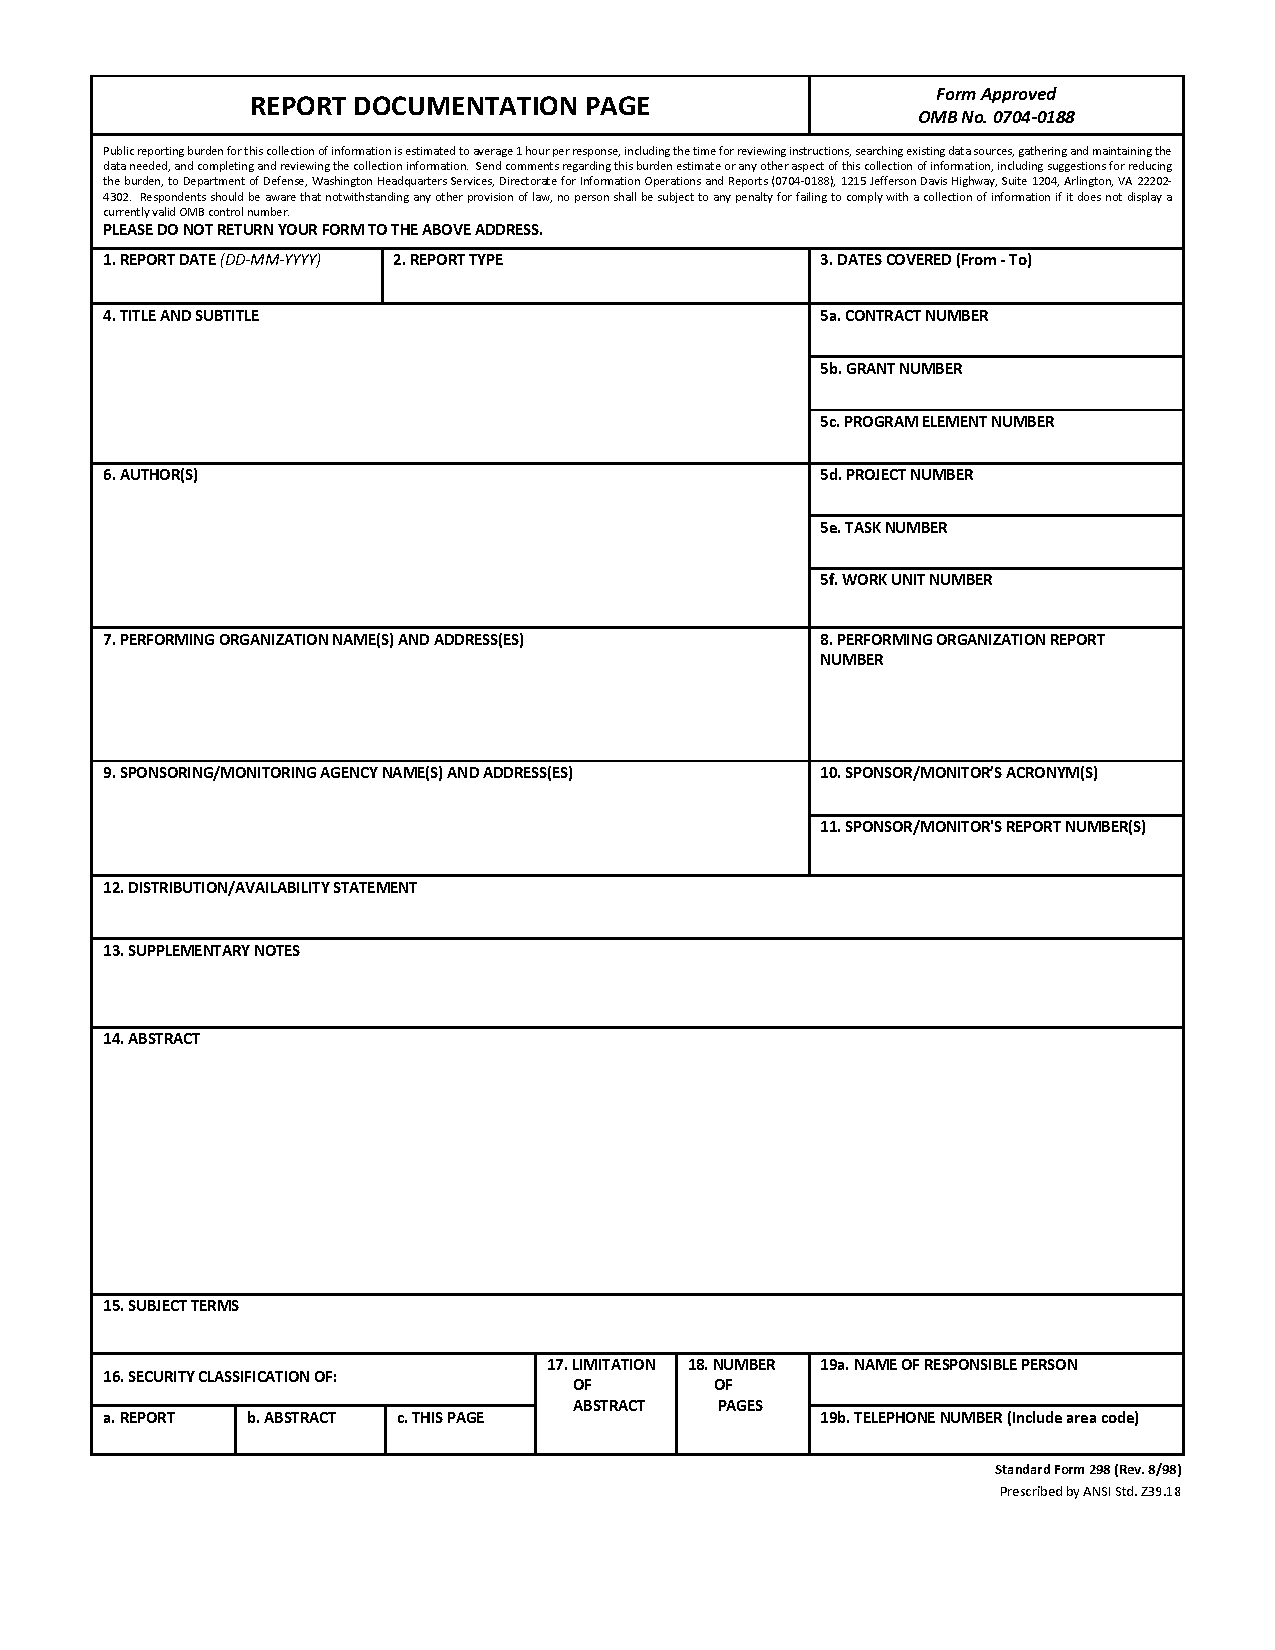
\includegraphics{SF298}
      \footnotesize
      \@SFitemONE{\@pubdate}
      \@SFitemTWO{\@reporttype}
      \@SFitemFOUR{\@arltitle}
      \@SFitemFIVEa{\Contract@Number}
      \@SFitemSIX{\@allauthors}
      \@SFitemEIGHT{\@arlrptno}
      \@SFitemTWELVE{\raggedright\@distribution}
      \def\SFitemSIXTEENaVALUE{Unclassified}
      \def\SFitemSIXTEENbVALUE{Unclassified}
      \def\SFitemSIXTEENcVALUE{Unclassified}
}{
      \put(-565,101){\parbox[c]{0.8in}{
          \SFitemSIXTEENaVALUE}}
      \put(-495,101){\parbox[c]{0.8in}{
          \SFitemSIXTEENbVALUE}}
      \put(-423,101){\parbox[c]{0.8in}{
          \SFitemSIXTEENcVALUE}}
      \put(-353,101){\parbox[c]{0.8in}{\centering
          \SFitemSEVENTEENvalue}}
      \normalsize
    \end{picture}
  \end{singlespace}
}
\newcommand\@SFitemONE[1]{\put(-564.5,656){#1}}
\newcommand\SFitemTWO[1]{\def\@reporttype{#1}}
\newcommand\@SFitemTWO[1]{\put(-424,656){#1}}
\newcommand\SFitemTHREE[1]{\put(-218,656){#1}}
\newcommand\@SFitemFOUR[1]{\put(-564.5,630){\parbox[t]{4.65in}{%
  \raggedright\def\\##1{\unskip\@sptoken##1}#1}}}
\newcommand\SFitemFOUR[1]{}
\newcommand\@SFitemFIVEa[1]{\put(-218,630){#1}}
\newcommand\SFitemFIVEb[1]{\put(-218,604){#1}}
\newcommand\SFitemFIVEc[1]{\put(-218,578){#1}}
\newcommand\SFitemFIVEd[1]{\put(-218,554){#1}}
\newcommand\SFitemFIVEe[1]{\put(-218,528){#1}}
\newcommand\SFitemFIVEf[1]{\put(-218,501){#1}}
\newcommand\@SFitemSIX[1]{\put(-564.5,554){\parbox[t]{4.65in}{%
  \raggedright\def\\##1{\unskip\@sptoken##1}#1}}}
\newcommand\SFitemSEVEN[1]{\put(-564.5,474){\parbox[t]{4.65in}{\raggedright#1}}}
\newcommand\@SFitemEIGHT[1]{\put(-218,462){#1}}
\newcommand\SFitemNINE[1]{\put(-564.5,412){\parbox[t]{4.65in}{\raggedright#1}}}
\newcommand\SFitemTEN[1]{\put(-218,410){#1}}
\newcommand\SFitemELEVEN[1]{\put(-218,383){#1}}
%FORMERLY: \newcommand\@SFitemTWELVE[1]
%  {\put(-564.5,355){\parbox[c]{7.15in}{\setstretch{0.8}#1}}}
\newcommand\@SFitemTWELVE[1]{%
  \setbox0=\hbox{\parbox[b]{7.15in}{\setstretch{0.8}#1}}%
  \ifdim\ht0>1.8\baselineskip%
    \put(-564.5,356){\scriptsize\parbox[c]{7.15in}{\setstretch{1.0}\hspace{160pt}#1}}%
  \else
    \ifdim\ht0>1.2\baselineskip%
      \put(-564.5,346){\scriptsize\parbox[b]{7.15in}{\setstretch{1.0}#1}}%
    \else%
      \put(-564.5,353){\parbox[c]{7.15in}{\setstretch{0.8}#1}}%
    \fi%
  \fi%
}
\newcommand\SFitemTHIRTEEN[1]{\put(-564.5,325){%
  \parbox[t]{7.1in}{\raggedright#1}}}
\newcommand\SFitemFOURTEEN[1]{\put(-564.5,282){%
  \parbox[t]{7.1in}{\raggedright#1}}}
\newcommand\SFitemFIFTEEN[1]{\put(-564.5,148){%
  \parbox[b]{7.1in}{\raggedright#1}}}
\newcommand\SFitemSIXTEENa[1]{\def\SFitemSIXTEENaVALUE{#1}}
\newcommand\SFitemSIXTEENb[1]{\def\SFitemSIXTEENbVALUE{#1}}
\newcommand\SFitemSIXTEENc[1]{\def\SFitemSIXTEENcVALUE{#1}}
\newcommand\SFitemSEVENTEEN[1]{}
\newcommand\SFitemEIGHTEEN[1]{\put(-285,101){\parbox[c]{0.8in}{\centering#1}}}
\newcommand\SFitemNINETEENa[1]{\put(-218,124){#1}}
\newcommand\SFitemNINETEENb[1]{\put(-218,99){#1}}

\SFitemTWO{Unknown Report Type}% DEFAULT SF298 ITEM 2
\def\@autodetectSFitemTWO#1-#2#3#4#5\relax{%
  \ifx-#4%
    \ifx R#3%
      \ifx T#2\SFitemTWO{Technical Report}\else%
        \ifx M#2\SFitemTWO{Memorandum Report}\else%
          \ifx S#2\SFitemTWO{Special Report}\else%
            \ifx C#2\SFitemTWO{Contractor Report}\else%
              \ifx I#2\SFitemTWO{Internal Report}%
      \fi\fi\fi\fi\fi%
    \else\ifx N#3%
      \ifx T#2\SFitemTWO{Technical Note}\fi%
    \else\ifx P#3%
      \ifx R#2\SFitemTWO{Reprint Report}\fi%
    \fi\fi\fi%
  \fi%
}
%
% NO LONGER PROVIDED AS OF V2.1
%
% The command \SFtwoNINEeight will draw a blank SF298 page, if no
% argument is provided.  The optional argument is used if the user has
% a filled out SF298 in the form of a EPS or PDF file.
%\newcommand\SFtwoNINEeight[1][SF298]{
%  \clearpage
%  \begin{picture}(612,650)(70,82)
%    \includegraphics{#1}
%  \end{picture}
%}
% Create a new command called \reportdocumentationpage that inserts a
% placeholder page for the report documentation page.
%
%\newcommand\reportdocumentationpage{
%  \clearpage
%  \begin{center}
%  \rule{0em}{0.5in}
%  REPLACE THIS PAGE WITH REPORT DOCUMENTATION PAGE (Standard Form 298)
%  \rule{0em}{2.0in}
%  \end{center}
%}
%REPLACE ABSTRACT ENVIRONMENT TO CONFORM WITH ARL STYLE
%\newcommand\theabstract{
%  \section*{\abstractname}
%  \newline
%  \newline
%}
%\newenvironment{abstract}{\theabstract\small}{\normalsize}

%%THE NEXT ENVIRONMENT ACCOUNTS FOR FOUR DIFFERENT SPELLINGS OF
%%  ACKNOWLEDGEMENT, ACKNOWLEDGEMENTS, ACKNOWLEDGMENT, ACKNOWLEDGMENTS
\newcommand \acknowledgement  {\def\ackname{%
  \spaceouthelpAcopy Acknowledgment \relax}  \ack}% SPACE BEFORE \relax IMPORTANT!!
\newcommand \acknowledgements {\def\ackname{%
  \spaceouthelpAcopy Acknowledgments \relax} \ack}% SPACE BEFORE \relax IMPORTANT!!
\newcommand \acknowledgment   {\def\ackname{%
  \spaceouthelpAcopy Acknowledgment \relax}  \ack}% SPACE BEFORE \relax IMPORTANT!!
\newcommand \acknowledgments  {\def\ackname{%
  \spaceouthelpAcopy Acknowledgments \relax} \ack}% SPACE BEFORE \relax IMPORTANT!!
%%INSERT NEW ENVIRONMENT FOR ack[knowledgment]
\newcommand\theack{\section*{\ClassificationLabel \ackname}}
\newenvironment{ack}{
  \clearpage
  \addcontentsline{toc}{section}{\ClassificationLabel \ackname}
  \theack}{}
\newcommand{\blankpage}{
  \clearpage
  \begin{center}
%   FORMERLY SMALL. NOW NORMALSIZE
    {\textsc{\rule{0em}{4.5in}Intentionally left blank.}}
  \end{center}
}

%% spaceout algorithm for section headings
\def\Letter@Gap{\kern\Letter@Space}
\newcommand\spaceout[2][\Letter@Space]{%
  \edef\tmp{\the\Letter@Space}%
  \setlength\Letter@Space{#1}%
  \spaceouthelpA#2{} \relax\relax%
  \setlength{\Letter@Space}{\tmp}%
}
\def\spaceouthelpA#1 #2\relax{%
  \spaceouthelpB#1{}\relax\relax%
  \ifx\relax#2\relax\else\ \Letter@Gap%
    \spaceouthelpA#2\relax\fi
}
\def\spaceouthelpB#1#2\relax{%
  \ifx\relax#2\relax#1\else
  \ifx#1\color\interceptColor#2\relax\relax\else
  \ifx#1\label\interceptLabel#2\relax\relax\else
      #1\protect\Letter@Gap\spaceouthelpB#2\relax%
  \fi\fi\fi%
}
\def\interceptColor#1#2\relax{%
  \color{#1}%
  \ifx\relax#2\else%
    \spaceouthelpB#2\relax%
  \fi%
}
\def\interceptLabel#1#2\relax{%
  \label{#1}%
  \ifx\relax#2\else%
    \spaceouthelpB#2\relax%
  \fi%
}
\def\sectspace{\let\spaceouthelpAcopy\spaceouthelpA}
\def\nosectspace{\let\spaceouthelpAcopy\relax}
\nosectspace

%% Redefine original commands called \section and \section* so as to place
%% ruler lines above and below section names in the ARL format for report 
%% sections
\newcommand\section{\@ifstar{\ruledheading}{\ruledsection}}
\newcommand\subsection{\@ifstar{\ruledsubheading}{\ruledsubsection}}
\newcommand\subsubsection{\@ifstar{\ARLsubsubheading}{\ARLsubsubsection}}
\newcommand\paragraph{\@ifstar{\ARLparaheading}{\ARLparagraph}}

%%\ruledsection is called by \section

\newcommand\ruledsection[1]{\sectionprelude\origsection{%
% THIS LINE FOR NON-STRETCHED SECTION HEADERS
%  #1%
% OR THIS LINE FOR STRETCHED SECTION HEADERS
  \spaceouthelpAcopy#1 \relax\relax%
%
  }\sectionpostlude
  \par%
}

\newcommand\ruledsubsection[1]{\bgroup\onehalfspacing%
  \subsectionprelude\origsubsection{#1}\subsectionpostlude\par\egroup%
}

\newcommand\ARLsubsubsection[1]{%
  \origsubsubsection{#1}\par\subsubsectionpostlude\par%
}

\newcommand\ARLparagraph[1]{%
  \origparagraph{#1}\par\paragraphpostlude\par%
}

%% \ruledheading is called by \section*
%% and is like \ruledsection, but unnumbered and un-toc'ed

\newcommand\ruledheading[1]{\bgroup\onehalfspacing%
  \sectionprelude\origsection*{%
% THIS LINE FOR NON-STRETCHED SECTION HEADERS
%  #1%
% OR THIS LINE FOR STRETCHED SECTION HEADERS
  \spaceouthelpAcopy#1 \relax\relax%
%
  }\sectionpostlude
  \par\egroup%
}

\newcommand\ruledsubheading[1]{\subsectionprelude%
  \origsubsection*{#1}\subsectionpostlude\par%
}

\newcommand\ARLsubsubheading[1]{%
  \origsubsubsection*{#1}\par\subsubsectionpostlude\par%
}

\newcommand\ARLparaheading[1]{%
  \origparagraph*{#1}\par\paragraphpostlude\par%
}

%%%%%

\newcommand\sectionprelude{%
  \needspace{\sectionSpaceMultiplier\defaultsectionspace}%
  \vspace{-6mm}%
  \def\sectionSpaceMultiplier{1}%
}
\newcommand\sectionpostlude{
  \vspace{-12mm}%
  {%
   \ooalign{\color{ReportColor}\rule{\textwidth}{1.6mm}%
    \cr\color{white}\rule[0.6mm]{\textwidth}{0.4mm}\cr}%
  }%
  \vspace{-3mm}
}
\newcommand\subsectionprelude{%
  \needspace{\sectionSpaceMultiplier\defaultsubsectionspace}%
  \def\sectionSpaceMultiplier{1}%
}
\newcommand\subsectionpostlude{
  \vspace{-9mm}%
  {%\color{ReportColor}%
    \rule{\textwidth}{0.01in}%
  }%
  \vspace{-3mm}
}

\newcommand\subsubsectionpostlude{\vspace{-3mm}}

\newcommand\paragraphpostlude{\vspace{-2mm}}

%% \baresection is like \section*, but is placed in the toc
\newcommand\baresection[1]{\section*{#1}\addcontentsline{toc}{section}{#1}}

%% See file header to read about \allocateSpaceOnce and \sectionSpaceMultiplier
\newlength\defaultsectionspace
\setlength\defaultsectionspace{5\baselineskip}
\newlength\defaultsubsectionspace
\setlength\defaultsubsectionspace{2\baselineskip}
\def\sectionSpaceMultiplier{1}
\newcommand\allocateSpaceOnce[1]{\def\sectionSpaceMultiplier{#1}}

%%
%% Create new bibliography environment that makes ruled section header
\newdimen\bibindent
\setlength\bibindent{1.5em}
\newenvironment{thebibliography}[1]
 {\section{\refname}\vspace*{-0.9em}%
  \@mkboth{\MakeUppercase\refname}{\MakeUppercase\refname}%
  \list{\@biblabel{\@arabic\c@enumiv}}%
       {\settowidth\labelwidth{\@biblabel{#1}}%
        \leftmargin\labelwidth
        \advance\leftmargin\labelsep
        \@openbib@code
        \usecounter{enumiv}%
        \let\p@enumiv\@empty
        \renewcommand\theenumiv{\@arabic\c@enumiv}}%
  \sloppy
  \clubpenalty4000
  \@clubpenalty \clubpenalty
  \widowpenalty4000%
  \sfcode`\.\@m}
 {\def\@noitemerr
   {\@latex@warning{Empty `thebibliography' environment}}%
  \endlist}
%% Redefine the appearance of bibliography labels for ARL style..
\renewcommand*{\@biblabel}[1]{#1.\hfill}
%THE FOLLOWING TWO LINES ARE INACTIVE WHEN USING THE cite STYLE PACKAGE
% Redefine the appearance of citation labels for ARL style.
%\renewcommand*{\@cite}[1]{(\textit{#1})}
%%
%% Define \arlbibliography, so that modified achemso style, named ARL
%% is utilized.  Abbreviated journal titles, by default
\newcounter{@loopindex}
\newcommand {\arlbibliography}[2][s p]{
  \clearpage
  \bibliographystyle{ARL}
  \def\journaltitles{journalshort}
  \def\statenames{statesfull}
  \getargs{#1}
  \setcounter{@loopindex}{0}
  \whiledo{\value{@loopindex} < \narg}{%  
    \addtocounter{@loopindex}{1}%
    \expandafter\edef\expandafter\@bibarg\expandafter{%
      \csname arg\roman{@loopindex}\endcsname}%
    \if f\@bibarg \def\journaltitles{journalfull} \fi
    \if p\@bibarg \def\statenames{statespostal} \fi
  }
  \bibliography{\journaltitles,\statenames,#2}
}
%% Create the environment \references which is used to list references in
%% a "verse" style, for those who don't use BiBTeX.
%%
\newcounter{refcount}
\newenvironment{references}
  {\clearpage \section{References}
   \begin{list}{\makebox[1.5em]{\arabic{refcount}.\hfill}}{
     \topsep -0.2em \leftmargin 1.6em \labelsep 0.1em \usecounter{refcount}}
  }
  {\end{list}}

\let\svthefootnote\thefootnote
\newcommand\freefootnote[1]{%
  \let\thefootnote\relax%
  \footnotetext{#1}%
  \let\thefootnote\svthefootnote%
}
%%
%% Create commands to create an unnumbered (lone) appendix or a series of
%% appendices, as needed
\newcommand\appendix{\@ifstar{\loneappendix}{\anappendix}}

\newcounter{appndx}
\setcounter{appndx}{0}

\newcommand\loneappendix[2][p]{
  \clearpage
  \refstepcounter{appndx}
  \setcounter{section}{\arabic{appndx}}
  \renewcommand\thesection {\appendixname~\Alph{appndx}.}
  \setcounter{subsection}{0}
  \renewcommand\thesubsection {\Alph{appndx}.\@arabic\c@subsection}
  \setcounter{paragraph}{0}
  \setcounter{subparagraph}{0}
  \setcounter{figure}{0}
  \renewcommand\thefigure{\Alph{appndx}-\@arabic\c@figure}
  \setcounter{table}{0}
  \renewcommand\thetable{\Alph{appndx}-\arabic{table}}
  \setcounter{equation}{0}
  \renewcommand\theequation {\Alph{appndx}-\arabic{equation}}
  \setcounter{footnote}{0}
  \def\appendixtitle{\appendixname. #2}
  \addcontentsline{toc}{section}\appendixtitle
  \if p#1\vspace*{\fill}\fi
  \theappendix\appendixtitle
  \if p#1\vspace*{\fill}\clearpage\fi
}

%% The following patch is needed to fix the use of the \p@<counter>
%% command
\renewcommand*\refstepcounter[1]{\stepcounter{#1}%
  \protected@edef\@currentlabel{%
    \csname p@#1\expandafter\endcsname
      \csname the#1\endcsname
  }%
}
\renewcommand{\p@appndx}[1]{\Alph{appndx}}

\newcommand\anappendix[2][p]{
  \clearpage
  \refstepcounter{appndx}
  \setcounter{section}{\arabic{appndx}}
  \renewcommand\thesection {\appendixname~\Alph{appndx}.}
  \setcounter{subsection}{0}
  \renewcommand\thesubsection {\Alph{appndx}.\@arabic\c@subsection}
  \setcounter{paragraph}{0}
  \setcounter{subparagraph}{0}
  \setcounter{equation}{0}
  \setcounter{figure}{0}
  \renewcommand\thefigure{\Alph{appndx}-\@arabic\c@figure}
  \setcounter{table}{0}
  \renewcommand\thetable{\Alph{appndx}-\arabic{table}}
  \renewcommand\theequation {\Alph{appndx}-\arabic{equation}}
  \setcounter{footnote}{0}
  \def\appendixtitle{\appendixname~\Alph{appndx}. #2}
  \addcontentsline{toc}{section}\appendixtitle
  \if p#1\vspace*{\fill}\fi
  \theappendix\appendixtitle
  \if p#1\vspace*{\fill}\clearpage\fi
}
\newcommand\theappendix[1]{
  \section*{\centering#1}
}
%% Create a new command called \distributionlistpage that inserts a
%% placeholder page for the Distribution List page.
\newcommand \distributionlistpage{
  \clearpage
  \addcontentsline{toc}{section}{\ClassificationLabel Distribution List}
  \begin{center}
  \rule{0em}{4.5in}
  REPLACE THIS PAGE WITH DISTRIBUTION LIST
  \end{center}
}
%
% As of V2.1, removed \DLPageStamp logic
%
% TO AUTOSET DISTLIST PAGESTAMP, SINCE CAN"T USE \PageStamp BETWEEN
% \distlistsetup AND \distlistcleanup
%\newcommand\DLPageStamp[1][UNCLASSIFIED]{%
%  \global\def\DLautoclass{T}\gdef\DFStampText{#1}%
%}
%\def\DLautoclass{F}

%% To create your own distribution list, first call on \distlistsetup
\newcommand\distlistsetup[1][w]{%
  \clearpage%
%  \if T\DLautoclass%
%    \def\thePageStamp{\DFStampText}%
%  \fi%
  \singlespace%
  \addcontentsline{toc}{section}{\ClassificationLabel Distribution List}%
  \newlength\itemsepSAVE%
  \let\itemsepSAVE\itemsep%
  \ifthenelse{\equal{x}{#1}}{}{%
    \def\f@open{\immediate\openout\tempfile=}%
    \edef\f@name{DL_\@arlrptno.tex}%
    \newwrite\tempfile%
    \expandafter\f@open\f@name%
    \immediate\write\tempfile{\noexpand\documentclass{arlticle}}%
    \immediate\write\tempfile{\noexpand\makeatletter}%
    \protected@iwrite\tempfile{\let\\\relax}%
        {\def\noexpand\noexpand\noexpand\@arltitle{\@arltitle}}
    \protected@iwrite\tempfile{\let\\\relax}%
        {\def\noexpand\noexpand\noexpand\@allauthors{\@allauthors}}
    \protected@iwrite\tempfile{\let\\\relax}%
        {\def\noexpand\noexpand\noexpand\@arlrptno{\@arlrptno}}
    \protected@iwrite\tempfile{\let\\\relax}%
        {\def\noexpand\noexpand\noexpand\@shortpubdate{\@shortpubdate}}
    \protected@iwrite\tempfile{\let\\\relax}%
        {\def\noexpand\noexpand\noexpand\MandatoryDL{\MandatoryDL}}
    \@ifundefined{LocalMandatoryDL}{}%
    {%
    \protected@iwrite\tempfile{\let\\\relax}%
        {\def\noexpand\noexpand\noexpand\LocalMandatoryDL{\LocalMandatoryDL}}
    }%
    \protected@iwrite\tempfile{\let\\\relax}%
        {\def\noexpand\noexpand\noexpand\UserDL{\UserDL}}
    \protected@iwrite\tempfile{\let\\\relax}%
        {\def\noexpand\noexpand\noexpand\ecwarningtext{\@ecwarningtext}}
    \@ifundefined{downgradeARGa}{}%
    {%
    \protected@iwrite\tempfile{\let\\\relax}%
        {\noexpand\noexpand\noexpand\downgrading%
          {\downgradeARGa}{\downgradeARGb}{\downgradeARGc}%
          {\downgradeARGd}{\downgradeARGe}}%
    }%
    \protected@iwrite\tempfile{\let\\\relax}%
        {\def\noexpand\noexpand\noexpand\@distribution{\@distribution}}
    \immediate\write\tempfile{\noexpand% DISTRIBUTION LIST MAKER DOCUMENT
% V1.01
%
% V1.00 - Initial release
% V1.01 - Uses \FOUOPageStamp, instead of \PageStamp
% V2.00 - Readied for New Report Cover, sans serif fonts (JAN 2015)
%
% This document will be \input, with the following data already preset:
%\documentclass {arlticle}
%\makeatletter 
%\def \@arltitle {}
%\def \@allauthors {}
%\def \@arlrptno {}
%\def \@pubdate {}
%\def \MandatoryDL {}
%\def \LocalMandatoryDL {}
%\def \UserDL {}
%\def \ecwarningtext {}
%\def \downgradetext {}
%\def \@distribution {}
%% DISTRIBUTION LIST MAKER DOCUMENT
% V1.01
%
% V1.00 - Initial release
% V1.01 - Uses \FOUOPageStamp, instead of \PageStamp
% V2.00 - Readied for New Report Cover, sans serif fonts (JAN 2015)
%
% This document will be \input, with the following data already preset:
%\documentclass {arlticle}
%\makeatletter 
%\def \@arltitle {}
%\def \@allauthors {}
%\def \@arlrptno {}
%\def \@pubdate {}
%\def \MandatoryDL {}
%\def \LocalMandatoryDL {}
%\def \UserDL {}
%\def \ecwarningtext {}
%\def \downgradetext {}
%\def \@distribution {}
%% DISTRIBUTION LIST MAKER DOCUMENT
% V1.01
%
% V1.00 - Initial release
% V1.01 - Uses \FOUOPageStamp, instead of \PageStamp
% V2.00 - Readied for New Report Cover, sans serif fonts (JAN 2015)
%
% This document will be \input, with the following data already preset:
%\documentclass {arlticle}
%\makeatletter 
%\def \@arltitle {}
%\def \@allauthors {}
%\def \@arlrptno {}
%\def \@pubdate {}
%\def \MandatoryDL {}
%\def \LocalMandatoryDL {}
%\def \UserDL {}
%\def \ecwarningtext {}
%\def \downgradetext {}
%\def \@distribution {}
%\input {DLprint.tex}
%\makeatother 

\usepackage{xcolor,stackengine}

\renewcommand\dlem[2][]{%
  \ifthenelse{\equal{}{#1}}{}{~\\~}%
  $\bigcirc$\textcolor{red}{\textbf{ #2}}%
  \ifthenelse{\equal{}{#1}}{\\}{}%
}

\begin{document}

\definecolor{brightgreen}{rgb}{0,.9,0}

\newsavebox{\doublestamp}
\savebox{\doublestamp}[6.in]
{\parbox{6.in}{\color{white}\bfseries\sffamily%
\begin{center}\huge For Official Use Only\end{center}}}%
\FOUOPageStamp[\usebox{\doublestamp}]
 
 \normalsize

 \makeatletter
 \def\@ecwarningtext{%
 {\large This document is %
 \textcolor{brightgreen}{\textsc{For Official Use Only}}\\~\\%
 The full report referenced above has the following distribution:}\\%
 \ecwarningtext~}%
 \def\@disclaimerpage{%
 \let\savethePageStamp\thePageStamp%
 \caseupper[e]{\thePageStamp}%
 \findwords[q]{\thestring}{CONFIDENTIAL}%
 \ifthenelse{\equal{\theresult}{0}}%
   {}{\def\thePageStamp{UNCLASSIFIED}}%
 \caseupper[e]{\thePageStamp}%
 \findwords[q]{\thestring}{SECRET}%
 \ifthenelse{\equal{\theresult}{0}}%
   {}{\def\thePageStamp{UNCLASSIFIED}}%
 }
 \makeatother

\let\svclearpage\clearpage
\def\clearpage{\let\clearpage\svclearpage}

 {\makebox[6.5in]{\Huge\color{white}\bfseries\sffamily%
  \smash{\raisebox{5pt}{\stackon{\large(with email addresses included)}%
  {Distribution List for ARL Report}}}}%
 }

\ARLcover{G}
\FOUOPageStamp

\underline{Files Used to Make This Distribution List:}

Mandatory Distribution: \MandatoryDL

Local Mandatory Distribution%
\makeatletter
\@ifundefined{LocalMandatoryDL}{ List is Undefined}{: \LocalMandatoryDL}
\makeatother

%% X-TENDED VERSION OF \dlitem, 3 ARGUMENTS, #3 CAN CONTAIN LINEBREAKS
%% AND APPEARS BELOW TOTAL COPY COUNT (WHICH IS ARGUMENT #2)
\renewcommand\xdlitem[3][\addressdefaultlines]{
  \setcounter{Lines}{#2}
  \addtocounter{Lines}{#2}
  \addtocounter{Lines}{#1}
  \setlength{\labelwidth}{0.61in}\setlength{\labelsep}{0.05in}%
  \item[\hfill%
    \tabcolsep=0pt\smash{\begin{tabular}[t]{c}#2\\#3\end{tabular}}%
  \hfill]
%% RESTORE ORIGINAL VALUES
  \setlength{\labelwidth}{0.31in}\setlength{\labelsep}{0.295in}%
  \needlines{\arabic{Lines}}
}

%% (PDF) VERSION OF \dlitem
\renewcommand\pdlitem[2][\addressdefaultlines]{
  \setcounter{Lines}{#2}
  \addtocounter{Lines}{#2}
  \addtocounter{Lines}{#1}
  \setlength{\labelwidth}{0.61in}\setlength{\labelsep}{0.05in}%
  \item[\hfill%
    \tabcolsep=0pt\smash{\begin{tabular}[t]{c}#2\\(PDF)\end{tabular}}%
  \hfill]
%% RESTORE ORIGINAL VALUES
  \setlength{\labelwidth}{0.31in}\setlength{\labelsep}{0.295in}%
  \needlines{\arabic{Lines}}
}

User Distribution: \UserDL

\distlistsetup[x]%         Set up page parameters for DL printing.
\begin{distributionlist}
  \input{\MandatoryDL}% Mandatory DL, Ensure you have current version
  \input{\UserDL}%          Your DL for this report.
\end{distributionlist}
\distlistcleanup%       Cleans up and restores pre-DL settings

\end{document}

%\makeatother 

\usepackage{xcolor,stackengine}

\renewcommand\dlem[2][]{%
  \ifthenelse{\equal{}{#1}}{}{~\\~}%
  $\bigcirc$\textcolor{red}{\textbf{ #2}}%
  \ifthenelse{\equal{}{#1}}{\\}{}%
}

\begin{document}

\definecolor{brightgreen}{rgb}{0,.9,0}

\newsavebox{\doublestamp}
\savebox{\doublestamp}[6.in]
{\parbox{6.in}{\color{white}\bfseries\sffamily%
\begin{center}\huge For Official Use Only\end{center}}}%
\FOUOPageStamp[\usebox{\doublestamp}]
 
 \normalsize

 \makeatletter
 \def\@ecwarningtext{%
 {\large This document is %
 \textcolor{brightgreen}{\textsc{For Official Use Only}}\\~\\%
 The full report referenced above has the following distribution:}\\%
 \ecwarningtext~}%
 \def\@disclaimerpage{%
 \let\savethePageStamp\thePageStamp%
 \caseupper[e]{\thePageStamp}%
 \findwords[q]{\thestring}{CONFIDENTIAL}%
 \ifthenelse{\equal{\theresult}{0}}%
   {}{\def\thePageStamp{UNCLASSIFIED}}%
 \caseupper[e]{\thePageStamp}%
 \findwords[q]{\thestring}{SECRET}%
 \ifthenelse{\equal{\theresult}{0}}%
   {}{\def\thePageStamp{UNCLASSIFIED}}%
 }
 \makeatother

\let\svclearpage\clearpage
\def\clearpage{\let\clearpage\svclearpage}

 {\makebox[6.5in]{\Huge\color{white}\bfseries\sffamily%
  \smash{\raisebox{5pt}{\stackon{\large(with email addresses included)}%
  {Distribution List for ARL Report}}}}%
 }

\ARLcover{G}
\FOUOPageStamp

\underline{Files Used to Make This Distribution List:}

Mandatory Distribution: \MandatoryDL

Local Mandatory Distribution%
\makeatletter
\@ifundefined{LocalMandatoryDL}{ List is Undefined}{: \LocalMandatoryDL}
\makeatother

%% X-TENDED VERSION OF \dlitem, 3 ARGUMENTS, #3 CAN CONTAIN LINEBREAKS
%% AND APPEARS BELOW TOTAL COPY COUNT (WHICH IS ARGUMENT #2)
\renewcommand\xdlitem[3][\addressdefaultlines]{
  \setcounter{Lines}{#2}
  \addtocounter{Lines}{#2}
  \addtocounter{Lines}{#1}
  \setlength{\labelwidth}{0.61in}\setlength{\labelsep}{0.05in}%
  \item[\hfill%
    \tabcolsep=0pt\smash{\begin{tabular}[t]{c}#2\\#3\end{tabular}}%
  \hfill]
%% RESTORE ORIGINAL VALUES
  \setlength{\labelwidth}{0.31in}\setlength{\labelsep}{0.295in}%
  \needlines{\arabic{Lines}}
}

%% (PDF) VERSION OF \dlitem
\renewcommand\pdlitem[2][\addressdefaultlines]{
  \setcounter{Lines}{#2}
  \addtocounter{Lines}{#2}
  \addtocounter{Lines}{#1}
  \setlength{\labelwidth}{0.61in}\setlength{\labelsep}{0.05in}%
  \item[\hfill%
    \tabcolsep=0pt\smash{\begin{tabular}[t]{c}#2\\(PDF)\end{tabular}}%
  \hfill]
%% RESTORE ORIGINAL VALUES
  \setlength{\labelwidth}{0.31in}\setlength{\labelsep}{0.295in}%
  \needlines{\arabic{Lines}}
}

User Distribution: \UserDL

\distlistsetup[x]%         Set up page parameters for DL printing.
\begin{distributionlist}
  \input{\MandatoryDL}% Mandatory DL, Ensure you have current version
  \input{\UserDL}%          Your DL for this report.
\end{distributionlist}
\distlistcleanup%       Cleans up and restores pre-DL settings

\end{document}

%\makeatother 

\usepackage{xcolor,stackengine}

\renewcommand\dlem[2][]{%
  \ifthenelse{\equal{}{#1}}{}{~\\~}%
  $\bigcirc$\textcolor{red}{\textbf{ #2}}%
  \ifthenelse{\equal{}{#1}}{\\}{}%
}

\begin{document}

\definecolor{brightgreen}{rgb}{0,.9,0}

\newsavebox{\doublestamp}
\savebox{\doublestamp}[6.in]
{\parbox{6.in}{\color{white}\bfseries\sffamily%
\begin{center}\huge For Official Use Only\end{center}}}%
\FOUOPageStamp[\usebox{\doublestamp}]
 
 \normalsize

 \makeatletter
 \def\@ecwarningtext{%
 {\large This document is %
 \textcolor{brightgreen}{\textsc{For Official Use Only}}\\~\\%
 The full report referenced above has the following distribution:}\\%
 \ecwarningtext~}%
 \def\@disclaimerpage{%
 \let\savethePageStamp\thePageStamp%
 \caseupper[e]{\thePageStamp}%
 \findwords[q]{\thestring}{CONFIDENTIAL}%
 \ifthenelse{\equal{\theresult}{0}}%
   {}{\def\thePageStamp{UNCLASSIFIED}}%
 \caseupper[e]{\thePageStamp}%
 \findwords[q]{\thestring}{SECRET}%
 \ifthenelse{\equal{\theresult}{0}}%
   {}{\def\thePageStamp{UNCLASSIFIED}}%
 }
 \makeatother

\let\svclearpage\clearpage
\def\clearpage{\let\clearpage\svclearpage}

 {\makebox[6.5in]{\Huge\color{white}\bfseries\sffamily%
  \smash{\raisebox{5pt}{\stackon{\large(with email addresses included)}%
  {Distribution List for ARL Report}}}}%
 }

\ARLcover{G}
\FOUOPageStamp

\underline{Files Used to Make This Distribution List:}

Mandatory Distribution: \MandatoryDL

Local Mandatory Distribution%
\makeatletter
\@ifundefined{LocalMandatoryDL}{ List is Undefined}{: \LocalMandatoryDL}
\makeatother

%% X-TENDED VERSION OF \dlitem, 3 ARGUMENTS, #3 CAN CONTAIN LINEBREAKS
%% AND APPEARS BELOW TOTAL COPY COUNT (WHICH IS ARGUMENT #2)
\renewcommand\xdlitem[3][\addressdefaultlines]{
  \setcounter{Lines}{#2}
  \addtocounter{Lines}{#2}
  \addtocounter{Lines}{#1}
  \setlength{\labelwidth}{0.61in}\setlength{\labelsep}{0.05in}%
  \item[\hfill%
    \tabcolsep=0pt\smash{\begin{tabular}[t]{c}#2\\#3\end{tabular}}%
  \hfill]
%% RESTORE ORIGINAL VALUES
  \setlength{\labelwidth}{0.31in}\setlength{\labelsep}{0.295in}%
  \needlines{\arabic{Lines}}
}

%% (PDF) VERSION OF \dlitem
\renewcommand\pdlitem[2][\addressdefaultlines]{
  \setcounter{Lines}{#2}
  \addtocounter{Lines}{#2}
  \addtocounter{Lines}{#1}
  \setlength{\labelwidth}{0.61in}\setlength{\labelsep}{0.05in}%
  \item[\hfill%
    \tabcolsep=0pt\smash{\begin{tabular}[t]{c}#2\\(PDF)\end{tabular}}%
  \hfill]
%% RESTORE ORIGINAL VALUES
  \setlength{\labelwidth}{0.31in}\setlength{\labelsep}{0.295in}%
  \needlines{\arabic{Lines}}
}

User Distribution: \UserDL

\distlistsetup[x]%         Set up page parameters for DL printing.
\begin{distributionlist}
  \input{\MandatoryDL}% Mandatory DL, Ensure you have current version
  \input{\UserDL}%          Your DL for this report.
\end{distributionlist}
\distlistcleanup%       Cleans up and restores pre-DL settings

\end{document}
}%
    \immediate\write\tempfile{\noexpand\makeatother}%
    \immediate\closeout\tempfile%
    \edef\@DLcompile{pdflatex \f@name}
    \if p#1\write18{\@DLcompile}\fi%
  }%
}

% CREATE DL TAB INDENT
\newcommand\dlt{\rule{0.92em}{0in}} % \dlt = [Distribution List Tab]

\newcommand\apg{\vspace{1.5em}\item\underline{ABERDEEN PROVING GROUND}}

\newcounter{Lines}
\def\addressdefaultlines{2}
\newcommand\dlitem[2][\addressdefaultlines]{
  \setcounter{Lines}{#2}
  \addtocounter{Lines}{#1}
  \item[#2]
  \needlines{\arabic{Lines}}
}


%% X-TENDED VERSION OF \dlitem, 3 ARGUMENTS, #3 CAN CONTAIN LINEBREAKS
%% AND APPEARS BELOW TOTAL COPY COUNT (WHICH IS ARGUMENT #2)
\newcommand\xdlitem[3][\addressdefaultlines]{
  \setcounter{Lines}{#2}
  \addtocounter{Lines}{#1}
  \setlength{\labelwidth}{0.61in}\setlength{\labelsep}{0.05in}%
  \item[\hfill%
    \tabcolsep=0pt\smash{\begin{tabular}[t]{c}#2\\#3\end{tabular}}%
  \hfill]
%% RESTORE ORIGINAL VALUES
  \setlength{\labelwidth}{0.31in}\setlength{\labelsep}{0.295in}%
  \needlines{\arabic{Lines}}
}

%% (PDF) VERSION OF \dlitem
\newcommand\pdlitem[2][\addressdefaultlines]{
  \setcounter{Lines}{#2}
  \addtocounter{Lines}{#1}
  \setlength{\labelwidth}{0.61in}\setlength{\labelsep}{0.05in}%
  \item[\hfill%
    \tabcolsep=0pt\smash{\begin{tabular}[t]{c}#2\\(PDF)\end{tabular}}%
  \hfill]
%% RESTORE ORIGINAL VALUES
  \setlength{\labelwidth}{0.31in}\setlength{\labelsep}{0.295in}%
  \needlines{\arabic{Lines}}
}

%% (HC) VERSION OF \dlitem
\newcommand\hdlitem[2][\addressdefaultlines]{
  \setcounter{Lines}{#2}
  \addtocounter{Lines}{#1}
  \setlength{\labelwidth}{0.61in}\setlength{\labelsep}{0.05in}%
  \item[\hfill%
    \tabcolsep=0pt\smash{\begin{tabular}[t]{c}#2\\(HC)\end{tabular}}%
  \hfill]
%% RESTORE ORIGINAL VALUES
  \setlength{\labelwidth}{0.31in}\setlength{\labelsep}{0.295in}%
  \needlines{\arabic{Lines}}
}

%% NEW \ldlitem, USES SAME CENTERING AS \xdlitem, \pdlitem, AND \hdlitem
\newcommand\ldlitem[2]{%
  \setlength{\labelwidth}{0.61in}\setlength{\labelsep}{0.05in}%
  \item[\hfill%
    \tabcolsep=0pt\smash{\begin{tabular}[t]{c}#1\\#2\end{tabular}}%
  \hfill]%
%% RESTORE ORIGINAL VALUES
  \setlength{\labelwidth}{0.31in}\setlength{\labelsep}{0.295in}%
}

\newcommand\dlem[2][1]{}

\newcommand\needlines[1]{\needspace{#1\baselineskip}} % With \item to allocate
%%                                                      space for full item
%
%% At end of distribution list, call on \distlistcleanup to restore
%% settings
\newcommand\distlistcleanup{
  \clearpage
  \onecolumn
  \pagestyle{\PlainStyle}
  \onehalfspacing%       Undoes the single spacing of the distribution list
  \if T\PageStampFlag%
    \def\PlainStyle{pagestamp}
    \def\EmptyStyle{emptypagestamp}
    \pagestyle{\PlainStyle}
%    \PageStamp[\thePageStamp]%
  \fi
}

%% After calling \distlistsetup, enter the distributionlist environment
%% to input your distribution list entries
%% Entries should be of the form:
%% \item [no. to distribute]
%% line 1\\
%% line 2\\
%% \dlt indented-line-as-needed
%%
\newenvironment{distributionlist}{
   \columnsep 0.2in
   \twocolumn
   \footnotesize
   \begin{list}{}{
     \setlength{\labelwidth}{0.24in}%
     \setlength{\labelsep}{0.29in}%
     \setlength{\leftmargin}{0.5in}%
     \setlength\itemsep{0.5em}
   }
  }
  {\setlength\itemsep{\itemsepSAVE}
   \clearpage
   \end{list}
   \normalsize
}

%% The pagestyle distlist and distlistend are obsolete
%% Reset to default page style if encountered
\let\ps@distlistend\ps@plain
\let\ps@distlist\ps@plain

%% \backcover prints out a totally blank page, for use as a report's
%% backcover
\newcommand\backcover{
  \clearpage
  \let\@abbrevdistribution\relax
%%  \pagecolor{\file@prefix ReportColor}% IF ONE WANTED COLORED BACK COVER
  \def\PageStampColor{black}% SINCE \@coverwhite TOO PALE
  \def\thePageStamp{}%
  \thispagestyle{\EmptyStyle}
  \textrm{}
  \clearpage
  \PageStamp[]
  \let\thePageStamp\savethePageStamp
  \thispagestyle{\EmptyStyle}
  \textrm{}
}

%Use \widow as last command in an affected paragraph
%Use \orphan as first command in affected paragraph
\newcommand\widow{%
  \widowpenalty=10000

  \widowpenalty=150}
\newcommand\orphan{%
  \needlines{2}%
}

%% To make single spacing following periods, colons, etc.
\frenchspacing

\usepackage{tocloft}
%%%%%%%%%%%%%%%%%%%%%%%%%%%%%%%%%%%%%%%%%%%%%%%%%%%%%%%%%%%%%%%%%%%%
%%
%% MODIFIED TOCLOFT PACKAGE TO FACILITATE PROPER FORMATTING OF
%% LISTS OF FIGURES AND TABLES IN THE ARL STYLE
%%
%%  Set \cftfigpresnum to "Fig.~" - this adds "Fig. " before each figure number in LOF
%%  Set \cfttabpresnum to "Table~" - this adds "Table " before each table number in LOT
%%
%%  Search for following commands to change values
%%  \setlength{\cftfigindent}{0in}       No indentation in LOF
%%  \setlength{\cftfignumwidth}{0.56in}  Width of box containing "Figure xx."
%%  \setlength{\cfttabindent}{0in}       No indentation in LOT
%%  \setlength{\cfttabnumwidth}{0.64in}  Width of box containing "Table xx."
%%  \setlength{\growloflabel}{0.em}          Extra width added to \cftfignumwidth
%%  \setlength{\growlotlabel}{0.em}	         and/or \cfttabnumwidth
%%					 to allow for wider caption widths
%%                                       from Figure or Table  A-1, etc. 
%%					 (set in document preamble).
%%
%% Modified \cfttabfillnum and \cftfigfillnum to do full dot leader.

\renewcommand{\cftdotsep}{0.6}

\renewcommand\cftsecfont{\bfseries\sffamily\Level@twosize}
\renewcommand\cftsubsecfont{\sffamily\Level@foursize}
\renewcommand\cftsubsubsecfont{\sffamily\Level@foursize}
\renewcommand\cftparafont{\sffamily\Level@foursize}
\renewcommand\cftsecpagefont{\bfseries\sffamily}
\renewcommand\cftsubsecpagefont{\sffamily\small}
\renewcommand\cftsubsubsecpagefont{\sffamily\footnotesize}
\renewcommand\cftparapagefont{\sffamily\footnotesize}
\renewcommand\cftsecaftersnum{.}

\setlength{\cftbeforesecskip}{0.5em \@plus\p@}
\setlength{\cftbeforesubsecskip}{-.5em \@plus\p@}
\setlength{\cftbeforesubsubsecskip}{-.5em \@plus\p@}
\setlength{\cftbeforeparaskip}{-.5em \@plus\p@}
\setlength{\cftbeforefigskip}{-.5em \@plus\p@}
\setlength{\cftbeforetabskip}{-.5em \@plus\p@}

\setlength{\cftfigindent}{0in}
\setlength{\cftfignumwidth}{0.56in}
\renewcommand{\cftfigpresnum}{Fig.~}
%% HACK \cftfigfillnum TO RUN DOT LEADER ALL THE WAY UP TO THE PAGE#
\renewcommand{\cftfigfillnum}[1]{%
  {\cftfigleader}\nobreak
%% \hb@xt@\@pnumwidth{\hfil\cftfigpagefont #1}\cftfigafterpnum\par}%ORIG
  \cftfigpagefont #1\cftfigafterpnum\par}

\setlength{\cfttabindent}{0in}
\setlength{\cfttabnumwidth}{0.64in}
\renewcommand{\cfttabpresnum}{Table~}
%% HACK \cfttabfillnum TO RUN DOT LEADER ALL THE WAY UP TO THE PAGE#
\renewcommand{\cfttabfillnum}[1]{%
  {\cfttableader}\nobreak
%% \hb@xt@\@pnumwidth{\hfil\cfttabpagefont #1}\cfttabafterpnum\par}%ORIG
  \cfttabpagefont #1\cfttabafterpnum\par}
%%%%%%%%%%%%%%%%%%%%%%%%%%%%%%%%%%%%%%%%%%%%%%%%%%%%%%%%%%%%%%%%%%%%

\def\tableofcontents{}
\def\listoffigures{}
\def\listoftables{}
\def\sec@star{\section*}
\AtBeginDocument{%
  \let\svnumberline\numberline%
  %%MODIFY TABLE OF CONTENTS TO INCLUDE RULE LINES
  %% ALSO, SCREEN OUT FREE FOOTNOTES IN SECTION TITLES FROM TOC
  \renewcommand\tableofcontents{%
    \let\svfreefootnote\freefootnote%
    \def\freefootnote##1{}%
    \clearpage%
%    THE FOLLOWING COMMENTED CODE ALLOWS DIST A REPORTS NOT TO HAVE ADDED FOOTER
%    HOWEVER, CURRENT GUIDANCE IS ALL REPORTS WILL CONTAIN DISTRIBUTION FOOTER
%    \if A\thedistcode\relax%
%      \newgeometry{hoffset=0pt,textwidth=5.5in,left=1.5in,right=1.5in,
%                   top=1in,bottom=1in}%
%    \else%
      \AddEverypageHook{\smash{\hspace*{%
          \dimexpr-\PageLeftMargin-\hoffset+1.5in\relax}%
        \raisebox{\dimexpr\PageTopMargin+\voffset-9.85in\relax}{%
          \textcolor{black!60}{%
        \parbox[t]{\textwidth}{\singlespacing\fontsize{7pt}{8pt}\selectfont%
          \sffamily\@abbrevdistribution}}}}}%
      \newgeometry{hoffset=0pt,textwidth=5.5in,left=1.5in,right=1.5in,%
                   top=1in,bottom=\dimexpr1in+10pt,%
                   footskip=\dimexpr\footskip+10pt}%
%    \fi
    \thetableofcontents%
    \let\freefootnote\svfreefootnote%
  }
  \newcommand\thetableofcontents{
    \section*{\contentsname}\vspace{-12pt}
    \renewcommand{\@pnumwidth}{1.0em}
    \begin{singlespace}
       \def\Letter@Gap{}
       \renewcommand\cftdotsep{10000}%
       \@starttoc{toc}%
    \end{singlespace}%
  }
  %%MODIFY \listoffigures" TO ADD TO TABLE OF CONTENTS & DRAW RULER LINES
  \renewcommand\listoffigures{\@ifstar{\@listoffigures[]}{\@listoffigures}}
  \newcommand\thelistoffigures{
    \section*{\listfigurename}\vspace{4pt}%
    \renewcommand{\@pnumwidth}{1.55em}
    \cftsetrmarg{0pt plus1fil}
    \if T\Single@Figure
        \def\numberline##1{\svnumberline{}}%
        \renewcommand{\cftfigpresnum}{Figure}
    \else
      \let\numberline\svnumberline
    \fi
    \begin{singlespace}
      \@starttoc{lof}%
    \end{singlespace}
  }
  %%MODIFY \listoftables" TO ADD TO TABLE OF CONTENTS & DRAW RULER LINES
  \renewcommand\listoftables{\@ifstar{\@listoftables[]}{\@listoftables}}
  \newcommand\thelistoftables{
    \section*{\listtablename}\vspace{4pt}%
    \renewcommand{\@pnumwidth}{1.55em}
    \cftsetrmarg{0pt plus1fil}
    \if T\Single@Table
      \def\numberline##1{\svnumberline{}}%
    \else
      \let\numberline\svnumberline
    \fi
    \begin{singlespace}
      \@starttoc{lot}%
    \end{singlespace}
  }
}
\newcommand\@listoffigures[1][\clearpage]{%
  #1%
  \addcontentsline{toc}{section}{\listfigurename}%
  \thelistoffigures%
}
\newcommand\@listoftables[1][\clearpage]{%
  #1%
  \addcontentsline{toc}{section}{\listtablename}%
  \thelistoftables%
}

\onehalfspacing

%    \end{macrocode}
% \Finale
\endinput
%%
%% End of file `arlticle.dtx'.
